\documentclass[11pt,a4paper,headinclude,footinclude,DIV16]{scrreprt}
\usepackage[usenames,dvipsnames,table]{xcolor} % include at beginning because of compitibility issues
\usepackage[english]{babel}
\usepackage[utf8]{inputenc}
\usepackage[automark]{scrpage2}
\usepackage[normalem]{ulem}
\usepackage{amsmath}
\usepackage{amsfonts}
\usepackage{amssymb}
\usepackage{booktabs}
\usepackage{enumerate}
\usepackage{hyperref}
\usepackage{graphicx}
\usepackage{listings}
\usepackage{makeidx}
\usepackage{pdflscape}
\usepackage{rotating}
\usepackage{subfig}
\usepackage{tabularx}
\usepackage{theorem}
\usepackage{tikz}
\usepackage{tikz-qtree}
\usepackage[colorinlistoftodos]{todonotes}
\usepackage{units}
\usepackage{url}
\usepackage{xspace}
\hypersetup{bookmarksdepth=3}
\usetikzlibrary{arrows}
\usetikzlibrary{backgrounds}
\usetikzlibrary{decorations.pathmorphing}
\usetikzlibrary{fit}
\usetikzlibrary{patterns}
\usetikzlibrary{positioning}
\usetikzlibrary{shapes}
\usetikzlibrary{trees}
\newcommand{\textcolordummy}[2]{#2}
\newcommand{\textcolordigits}{\textcolor{Mulberry}}
\lstset{showstringspaces=false,
 inputencoding=ansinew,
 breaklines=true,
 tabsize=4,
 columns=flexible,
 literate={0}{{\textcolordigits{0}}}{1}%
          {1}{{\textcolordigits{1}}}{1}%
          {2}{{\textcolordigits{2}}}{1}%
          {3}{{\textcolordigits{3}}}{1}%
          {4}{{\textcolordigits{4}}}{1}%
          {5}{{\textcolordigits{5}}}{1}%
          {6}{{\textcolordigits{6}}}{1}%
          {7}{{\textcolordigits{7}}}{1}%
          {8}{{\textcolordigits{8}}}{1}%
          {9}{{\textcolordigits{9}}}{1}%
          {.0}{{\textcolordigits{.0}}}{2}% Following is to ensure that only periods
          {.1}{{\textcolordigits{.1}}}{2}% followed by a digit are changed.
          {.2}{{\textcolordigits{.2}}}{2}%
          {.3}{{\textcolordigits{.3}}}{2}%
          {.4}{{\textcolordigits{.4}}}{2}%
          {.5}{{\textcolordigits{.5}}}{2}%
          {.6}{{\textcolordigits{.6}}}{2}%
          {.7}{{\textcolordigits{.7}}}{2}%
          {.8}{{\textcolordigits{.8}}}{2}%
          {.9}{{\textcolordigits{.9}}}{2}%
          {e0}{{\textcolordigits{e0}}}{2}% Following is to ensure that only periods
          {e1}{{\textcolordigits{e1}}}{2}% followed by a digit are changed.
          {e2}{{\textcolordigits{e2}}}{2}%
          {e3}{{\textcolordigits{e3}}}{2}%
          {e4}{{\textcolordigits{e4}}}{2}%
          {e5}{{\textcolordigits{e5}}}{2}%
          {e6}{{\textcolordigits{e6}}}{2}%
          {e7}{{\textcolordigits{e7}}}{2}%
          {e8}{{\textcolordigits{e8}}}{2}%
          {e9}{{\textcolordigits{e9}}}{2}%
          {e-0}{{\textcolordigits{e-0}}}{2}% Following is to ensure that only periods
          {e-1}{{\textcolordigits{e-1}}}{2}% followed by a digit are changed.
          {e-2}{{\textcolordigits{e-2}}}{2}%
          {e-3}{{\textcolordigits{e-3}}}{2}%
          {e-4}{{\textcolordigits{e-4}}}{2}%
          {e-5}{{\textcolordigits{e-5}}}{2}%
          {e-6}{{\textcolordigits{e-6}}}{2}%
          {e-7}{{\textcolordigits{e-7}}}{2}%
          {e-8}{{\textcolordigits{e-8}}}{2}%
          {e-9}{{\textcolordigits{e-9}}}{2},
}

% for listings of bash code
\lstdefinestyle{Bash}{
 language=Bash,
 backgroundcolor=\color{lightgray},
 basicstyle=\ttfamily\small\let\textcolor\textcolordummy,
 numbers=none,
 captionpos=b,
 tabsize=4,
 frame=single,
 rulecolor=\color{lightgray},
 framerule=1pt,
 framesep=1pt,
 rulesep=0pt,
 aboveskip=\bigskipamount,
 belowskip=\bigskipamount
}

% for listings of shell code
\lstdefinestyle{Shell}{
 language=sh,
 numbers=left,
 numbersep=5pt,
 numberstyle=\tiny\noncopynumber,
 basicstyle=\ttfamily\scriptsize,
 stringstyle=\color{BrickRed}\ttfamily\let\textcolor\textcolordummy,
 commentstyle=\color[gray]{0.35}\ttfamily\itshape\let\textcolor\textcolordummy,
}

% for listings of DuMuX code
\lstdefinestyle{DumuxCode}{
  language=C++,
  extendedchars=true,
  escapeinside={/*@}{@*/}, % escape the long comments
  numbers=left,
  numbersep=5pt,
  numberstyle=\tiny\noncopynumber,
  basicstyle=\ttfamily\scriptsize,
  keywordstyle=\color{dumuxBlue}\ttfamily\let\textcolor\textcolordummy,
  stringstyle=\color{BrickRed}\ttfamily\let\textcolor\textcolordummy,
  commentstyle=\color[gray]{0.35}\ttfamily\itshape\let\textcolor\textcolordummy,
  emph={NEW_TYPE_TAG, NEW_PROP_TAG, UNSET_PROP, TTAG, PTAG,
       SET_PROP, GET_PROP, GET_PROP_VALUE, GET_PROP_TYPE,
       SET_BOOL_PROP, SET_STRING_PROP, SET_SCALAR_PROP, SET_TYPE_PROP, SET_INT_PROP,
       GET_BOOL_PROP, GET_STRING_PROP, GET_SCALAR_PROP, GET_TYPE_PROP, GET_INT_PROP,
       GET_PARAM, GET_PARAM_FROM_GROUP, GET_RUNTIME_PARAM, GET_RUNTIME_PARAM_FROM_GROUP},
  emphstyle=\color{OliveGreen}\let\textcolor\textcolordummy,
  directivestyle=\color{Brown}\ttfamily\let\textcolor\textcolordummy,
}

% for listings of DuMuX parameter files
\lstdefinestyle{DumuxParameterFile}{
 language=sh,
 numbers=left,
 numbersep=5pt,
 numberstyle=\tiny\noncopynumber,
 basicstyle=\ttfamily\scriptsize,
 stringstyle=\color{BrickRed}\ttfamily\let\textcolor\textcolordummy,
 commentstyle=\color[gray]{0.35}\ttfamily\itshape\let\textcolor\textcolordummy,
 morecomment=[l][\color{dumuxBlue}\let\textcolor\textcolordummy]{[},
}

\newcommand{\noncopynumber}[1]{
    \BeginAccSupp{method=escape,ActualText={}}
    #1
    \EndAccSupp{}
}


\DeclareGraphicsExtensions{.pdf, .jpg}

% Dune and Dumux logo
\newcommand{\Dune}{{DUNE}\xspace}
\newcommand{\Dumux}{\texorpdfstring{Du\-Mu$^\text{x}$\xspace}{DuMuX\xspace}}
\newcommand{\DumuxVersion}{2.8}
\definecolor{dumuxYellow}{HTML}{E19417}
\definecolor{dumuxBlue}{HTML}{0C73CF}

% sytles
\newcommand{\nextline}{\par\phantom{a}\vspace*{0.1\textwidth}}
\newcommand{\snakeline}{\uwave{\mbox{}}}
\DeclareRobustCommand\Cplusplus{\texorpdfstring{C\nolinebreak[4]\hspace{-.05em}\raisebox{.4ex}{\tiny\bf ++}\xspace}{C++}}

% notation
\newcommand{\porosity}{\phi}
\newcommand{\saturation}{S}

% a new counter you can give a label to it and thus reference it
% syntax: \numberThis{printedTextToBeLabeled}{label}
% if you wanted a \newline after a numbered thing, you could just add a empty line after ``\label{#2}''
\newcounter{thingCounter}
\renewcommand{\thethingCounter}{\arabic{thingCounter}}
\newcommand{\numberThis}[2]{%
        \refstepcounter{thingCounter}%
        \thethingCounter.\ #1 \label{#2}
}

%The theorems
\theorembodyfont{\upshape}
\theoremheaderfont{\sffamily\bfseries}
\newtheorem{lst}{Listing}

\DeclareMathOperator{\grad}{\bf grad}
\DeclareMathOperator{\curl}{curl}
\DeclareMathOperator{\Div}{div}

\pagestyle{scrheadings}

\title{
\begin{center}

\includegraphics[width=0.7\textwidth]{../logo/dumux_logo_hires_whitebg.png}
\\[3cm]
{\Huge Handbook}
\end{center}
}

\author{}

\date{Version \DumuxVersion}

\publishers{%
\vspace{10mm}
{\normalsize Lehrstuhl f\"ur Hydromechanik und Hydrosystemmodellierung, \\
Universit\"at Stuttgart, Paffenwaldring 61, D-70569 Stuttgart, Germany}\\
%
\bigskip
{\normalsize \texttt{\url{http://dumux.org}}}\\
}

\makeindex

\begin{document}

\maketitle

\setcounter{tocdepth}{1}
% \pdfbookmark[0]{Table of Contents}{Table of Contents}
\tableofcontents

\newpage
\pdfbookmark[1]{List of ToDos}{List of ToDos}
% \makeatletter\let\chapter\@undefined\makeatother
\listoftodos

\chapter*{Discussion about the new handbook}
\todo[inline]{Ihr konnt die todo Befehle benutzen um Dinge zu markieren, die euch
  auffallen, dann können wir die beim nachsten Mal besprechen}
\section*{Beschlossene ToDos}
DEADLINE: 29.07.15
\begin{itemize}
  \item Modelle raus, Liste rein (Christoph)
  \item Neues Gitterkapitel (Natalie)
  \begin{itemize}
    \item gmesh (Timo)
    \item petrel (Alex)
    \item[x] artgridcreator (Nicolas)
    \item[x] dgf (kurz kommentieren)
    \item[x] icemcfd (nicolas)
  \end{itemize}
  \item Wiki
  \begin{itemize}
    \item[+] behandla, Mailing list (LH2), external Modules, lectures, tests
             teilweise schon erledigt -$>$ Rest (Vishal)
    \item[+] Infos fur neue Doktoranden (Christoph)
  \end{itemize}
  \item Hinweis auf tests, lecture und feature list am Ende von Tutorial
        (Gaby)
  \item[x] Doxygen (main page - link auf modules, featureList und parameterList)
        (Kilian)
  \item Newton etwas ausfuhrlicher und Dumux spezifischer, schematische
        Skizze der Matrix (Christoph)
  \item[x] Kapitel 4 weiter aufräumen (Christoph+Thomas)
  \begin{itemize}
    \item Tips und Tricks weiter integrieren
    \item Reihenfolge der Unterkapitel
  \end{itemize}
  \item[x] Kapitel 5 weiter aufräumen (Christoph+Thomas)
  \begin{itemize}
    \item Reihenfolge der Unterkapitel
    \item \Dumux aus den Uberschriften in Kap 5 rausnehmen
  \end{itemize}
  \item[x] release manager tasks + tutorials anschauen/testen (Thomas)
  \item Rechtschreibung - pdf in word öffnen
\end{itemize}

\section*{Weitere ToDos}
\begin{itemize}
  \item Kapitel 5: Unterkapitel aufteilen -$>$ weiter aufräumen (s. Todos)
\end{itemize}

\section*{Offene Fragen}
\begin{itemize}
  \item Was kann ins Wiki ausgelagert werden?
  \item Was kann ins doxygen ausgelagert werden?
  \item Alles was (nicht?) LH2 spezifische raus?
  \item Fur listOfProperties und listOfFeatures auf doxygen verweisen! (kommt
        unter doxygen main pages)
  \item Modelbeschreibungen rausschmeißen?
  \item bennenung der ausgelagerten tex dateien mit kapitelnummer (nur eine nummer)
        beginnend
  \item Neue Kapitel/Abschnitte
  \begin{itemize}
    \item Wie kann ich Gitter erstellen (externe tools), /einlesen (dune), wo
          kann ich bei dune nachschauen. Welche Dateien werden uberhaupt unterstutzt?
          in Kap 5 (jemanden finden, der sich auskennt Alex, Timo, Bernd)
  \end{itemize}
  \item Tutorials:
  \begin{itemize}
    \item Noch aktuell, noch funktioniert?
    \item Welche Features, Modelle brauchten auch ein Tutorial? Wie konnen wir
          den Einstieg leicht machen und fur uns den Aufwand gering halten?
    \item Verweis auf lecture fur realistischere Anwendungen
  \end{itemize}
\end{itemize}

\section*{Erledigt}
\begin{itemize}
  \item leer
\end{itemize}


\chapter{Introduction}
\Dumux aims to be a generic framework for the simulation of multiphase
fluid flow and transport processes in porous media using continuum
mechanical approaches.  At the same time, \Dumux aims to deliver
top-notch computational performance, high flexibility, a sound
software architecture and the ability to run on anything from single
processor systems to highly parallel supercomputers with specialized
hardware architectures.

The means to achieve these somewhat contradictory goals are the
thorough use of object-oriented design in conjunction with template
programming. These requirements call for \Cplusplus as the implementation
language.

One of the more complex issues when dealing with parallel continuum
models is managing the grids used for the spatial discretization of
the physical model. To date, no generic and efficient approach exists
for all possible cases, so \Dumux is build on top of \Dune, the
\textbf{D}istributed and \textbf{U}nified \textbf{N}umerics
\textbf{E}nvironment~\cite{DUNE-HP}. \Dune provides a generic interface
to many existing grid management libraries such as UG~\cite{UG-HP},
ALUGrid~\cite{ALUGRID-HP,alugrid2016} and a few more.
DUNE also extensively uses template programming in order to
achieve minimal overhead when accessing the underlying grid
libraries\footnote{In fact, the performance penalty resulting from the
use of \Dune's grid interface is usually negligible~\cite{BURRI2006}.}.
\begin{figure}[hbt]
  \centering
  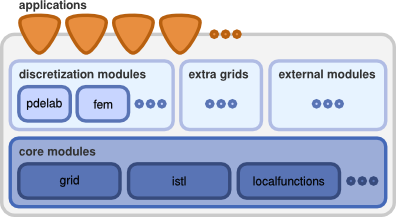
\includegraphics[width=.5\linewidth, keepaspectratio]{png/dunedesign.png}
  \caption{
    \label{fig:dune-design}
    A high-level overview of \Dune's design is available on the project's
    web site~\cite{DUNE-HP}.
  }
\end{figure}

DUNE's grid interface is independent of the spatial dimension of the
underlying grid. For this purpose, it uses the concept of
co-dimensional entities. Roughly speaking, an entity of co-dimension
$0$ constitutes a cell, co-dimension $1$ entities are faces between
cells, co-dimension $2$ are edges, and so on until co-dimension $n$
which are the cell's vertices.  The \Dune grid interface generally
assumes that all entities are convex polytopes, which means that it
must be possible to express each entity as the convex hull of a set of
vertices. For the sake of efficiency, all entities are further expressed in terms
of so-called reference elements which are transformed to the actual
spatial incarnation within the grid by a so-called geometry
function. Here, a reference element for an
entity can be thought of as a prototype for the actual grid
entity. For example, if we used a grid which applied hexahedrons as cells,
the reference element for each cell would be the unit cube $[0, 1]^3$
and the geometry function would scale and translate the cube so that
it matches the grid's cell. A quick overview of reference elements and the
related numbering can be obtained from the DUNE cheat sheet
(\url{https://www.dune-project.org/pdf/dune-cheat-sheet.pdf}).
For a more thorough description of \Dune's
grid definition, see~\cite{BASTIAN2008}.

In addition to the grid interface, \Dune also provides quite a few
additional modules, of which the \texttt{dune-localfunctions} and
\texttt{dune-istl} modules are the most relevant in the context of
this handbook. \texttt{dune-localfunctions} provides a set of generic
finite element shape functions, while \texttt{dune-istl} is the
\textbf{I}terative \textbf{S}olver \textbf{T}emplate \textbf{L}ibrary
and provides generic, highly optimized linear algebra routines for
solving the generated systems.

\Dumux comes in form of an additional module \texttt{dumux}.
It depends on the \Dune core modules
\texttt{dune-common}, \texttt{dune-grid}, \texttt{dune-istl}, and \texttt{dune-localfunctions}.
The main intention of \Dumux is to provide a framework for an easy and efficient
implementation of new physical models for porous media flow problems,
ranging from problem formulation and the selection of
spatial and temporal discretization schemes as well as nonlinear solvers,
to general concepts for model coupling.
Moreover, \Dumux includes ready to use numerical models and a few example applications.

This is the handbook to a new minor version update of \Dumux: version 3.1.
The release contains improvements and new features compared to the 3.0 version.
The update is  backwards compatible with the last release 3.0.
To facilitate the transition for our users, we have created a changelog
helping to update programs from version 3.0 to version 3.1, and giving an overview over new capabilities.
It is available online:
\url{https://git.iws.uni-stuttgart.de/dumux-repositories/dumux/blob/master/CHANGELOG.md}.
We highly recommend all our users to transition with us to the most recent version of \Dumux
and wish everyone a brand-new and exciting simulation experience.


\chapter{Getting started}
First, we describe a quick installation procedure.
Then a quick start guide for the first \Dumux experience is provided.
\section{Prerequisites} \label{sec:prerequisites}
For this quick start guide the following software packages are required:
\begin{itemize}
\item GitLab client
\item A standard compliant C++ compiler supporting C++11 and the C++14 feature set of GCC 4.9. We support GCC 4.9 or newer and Clang 3.8 or newer.
\item CMake 2.8.12 or newer
\item pkg-config
\item ParaView (to visualize the results)
\end{itemize}

\section{Obtaining code and configuring all modules with a script}
We provide you with a shell-script \texttt{installDumux.sh} that facilitates setting up a {\Dune}/{\Dumux} directory tree
and configures all modules with CMake.
Copy the following lines into a text file named \texttt{installDumux.sh}:
\lstinputlisting[style=DumuxCode, numbersep=5pt, firstline=1, firstnumber=1]{installDumux.sh}

Place the \texttt{installDumux.sh} script in the directory where you want to install \Dumux and \Dune (a single
root folder \texttt{DUMUX} will be produced, so you do not need to provide one). Make \texttt{installDumux.sh} executable and run the script by typing into the terminal: \texttt{./installDumux.sh}

Configuring \Dune and \Dumux is done by the command-line script \texttt{dunecontrol}
using optimized configure options, see the line entitled \texttt{\# run build} in the \texttt{installDumux.sh} script.
More details about the build-system can be found in section \ref{buildIt}.

\subsection{A first test run of \Dumux}
When the \texttt{installDumux.sh} script from the subsection above has run successfully, you can execute a second script that
will compile and run a simple one-phase ground water flow example and will visualize the result using ParaView.
The test script can be obtained by copying the following lines into a text file named \texttt{test\_dumux.sh}
that has to be located in the same directory as the installation script.
\begin{lstlisting}[style=DumuxCode]
cd DUMUX/dumux/build-cmake/test/porousmediumflow/1p/implicit/isothermal
make -B test_1p_tpfa
./test_1p_tpfa params.input
paraview *pvd
\end{lstlisting}
After making \texttt{test\_dumux.sh} executable, it can be executed by typing into the terminal: \texttt{./test\_dumux.sh}.
If everything works fine, a ParaView window with the result should open automatically, showing the initial
conditions. Advance ParaView to the next frame (green arrow button) and rescale to data range (green double arrow on top right) to admire
the colorful pressure distribution.

\section[Quick Start Guide]{Quick Start Guide: The First Run of a Test Application}
\label{quick-start-guide}

The previous section showed how to install and compile \Dumux. This chapter
shall give a very brief introduction how to run a first test application and how
to visualize the first output files. A more detailed explanations can be found in
the tutorials in the following chapter.\\
All executables are compiled in the \texttt{build} subdirectories of \Dumux.
If not given differently in the input files, this is \texttt{build-cmake} as default.

\begin{enumerate}
\item Go to the directory \texttt{build-cmake/test}. There, various test application
      folders can be found. Let us consider as example \texttt{porousmediumflow/2p/implicit/test{\_}box2p}:
\item Enter the folder \texttt{porousmediumflow/2p/implicit}. Type \texttt{make test{\_}box2p} in order
      to compile the application \texttt{test{\_}box2p}. To run the simulation, type\\
      \texttt{./test{\_}box2p -parameterFile ./test\_box2p.input}\\
      into the console. The parameter \texttt{-parameterFile} specifies that all
      important parameters (like first timestep size, end of simulation and location
      of the grid file) can be found in a text file in the same directory  with the
      name \texttt{test\_box2p.input}.
\item The simulation starts and produces some .vtu output files and also a .pvd
      file. The .pvd file can be used to examine time series and summarizes the .vtu
      files. It is possible to stop a running application by pressing $<$Ctrl$><$c$>$.
\item You can display the results using the visualization tool ParaView (or
      alternatively VisIt). Just type \texttt{paraview} in the console and open the
      .pvd file. On the left hand side, you can choose the desired parameter to be displayed.
\end{enumerate}

% \section{Detailed Installation Instructions}
% \label{install}

Installing \Dumux means that you first unpack \Dune and \Dumux in a root directory,
(section \ref{sc:ObtainingSourceCode}).
In a second step of the installation, all modules are configured with CMake
(section \ref{buildIt}).
After successfull installation of \Dumux we guide you to start a test application,
described in section \ref{quick-start-guide}.
In section \ref{sec:build-doxy-doc} we explain how to build the \Dumux documentation.
Lastly, section \ref{sec:external-modules-libraries} provides details on optional libraries and modules.

In a technical sense \Dumux is a module of \Dune.
Thus, the installation procedure of \Dumux is the same as that of \Dune.
Details regarding the installation of \Dune are provided on the \Dune website \cite{DUNE-HP}.


\section{Obtaining Source Code for \Dune and \Dumux}
\label{sc:ObtainingSourceCode}
The \Dumux release and trunk (developer tree) are based on the most recent
\Dune release 2.6, comprising the core modules dune-common, dune-geometry, dune-grid,
dune-istl and dune-localfunctions. For working with \Dumux, these modules are required.
All \Dune modules, including the \Dumux module, get extracted into a common root directory, as it
is done in an ordinary \Dune installation.
We usually name our root directory \texttt{DUMUX} but an arbitrary name can be chosen.
Source code files for each \Dune module are contained in their own subdirectory within the root directory.
The subdirectories for the modules are named after the module names (depending on how
the modules were obtained a version number is added to the module name).
The name of each \Dune module is defined in the file \texttt{dune.module}, which is
in the root directory of the respective module. This should not be changed by the user.

Two possibilities exist to get the source code of \Dune and \Dumux.
Firstly, \Dune and \Dumux can be downloaded as tar files from the respective \Dune and \Dumux website.
They have to be extracted as described in the next paragraph.
% % TODO: alpha version was not released with a tarball. For the next releases the following lines need to be deleted again
% There is no tar file for the current \DumuxVersion~release.
% Secondly, a method to obtain the most recent source code (or, more generally, any of its previous revisions) by direct access
% to the software repositories of the revision control system is described in the subsequent part.
% Be aware that you cannot get \texttt{dumux-devel} or the external libraries from \texttt{dumux-external} unless
% you have an GitLab account with the right privileges.

In section \ref{sec:prerequisites} we list some prerequisites for running \Dune and \Dumux.
Please check in said paragraph whether you can fulfill them before continuing.

% TODO: alpha version was not released with a tarball. For the next releases the following lines need to be uncommented again
\paragraph{Obtaining the software by installing tar files}
The slightly old-fashionedly named tape-archive-file, shortly named tar file or
tarball, is a common file format for distributing collections of files contained
within these archives.
The extraction from the tar files is done as follows:
Download the tarballs from the respective \Dune (version 2.6) and \Dumux websites
to a certain folder in your file system.
Create the common root directory, named \texttt{DUMUX} in the example below.
Then extract the content of the tar files, e.\,g. with the command-line program
\texttt{tar}.
This can be achieved by the following shell commands. Replace \texttt{path\_to\_tarball}
with the directory name where the downloaded files are actually located.
After extraction, the actual name of the dumux subdirectory is \texttt{dumux-\DumuxVersion}
(or whatever version you downloaded).

\begin{lstlisting}[style=Bash]
$ mkdir DUMUX
$ cd DUMUX
$ tar xzvf path_to_tarball_of/dune-common-2.6.0.tar.gz
$ tar xzvf path_to_tarball_of/dune-geometry-2.6.0.tar.gz
$ tar xzvf path_to_tarball_of/dune-grid-2.6.0.tar.gz
$ tar xzvf path_to_tarball_of/dune-istl-2.6.0.tar.gz
$ tar xzvf path_to_tarball_of/dune-localfunctions-2.6.0.tar.gz
$ tar xzvf path_to_tarball_of/dumux-3.0.tar.gz
\end{lstlisting}

Furthermore, if you wish to install the optional \Dune Grid-Howto which provides a tutorial
on the Dune grid interface, act similar.

\paragraph{Obtaining \Dune and \Dumux from software repositories}
Direct access to a software revision control system for downloading code can be of advantage later on.
It is easier to keep up with code changes and to receive important bug fixes.
\Dune and \Dumux use Git for their software repositories. To access them a Git client is needed.

In the technical language of Git, \emph{cloning a certain software version} means nothing more then fetching
a local copy from the software repository and laying it out in the file system.
In addition to the software, some more files for the use of the software revision
control system itself are created. If you have developer access to \Dumux, it is
also possible to do the opposite, i.\,e. to load up a modified revision of software
into the software repository. This is usually termed as \emph{commit} and \emph{push}.

The installation procedure is done as follows:
Create a common root directory, named e.g. \texttt{DUMUX} in the lines below.
Then, enter the previously created directory and check out the desired modules.
As you see below, the check-out uses two different servers for getting the sources,
one for \Dune and one for \Dumux.

\begin{lstlisting}[style=Bash]
$ mkdir DUMUX
$ cd DUMUX
$ git clone -b releases/2.6 https://gitlab.dune-project.org/core/dune-common.git
$ git clone -b releases/2.6 https://gitlab.dune-project.org/core/dune-geometry.git
$ git clone -b releases/2.6 https://gitlab.dune-project.org/core/dune-grid.git
$ git clone -b releases/2.6 https://gitlab.dune-project.org/core/dune-istl.git
$ git clone -b releases/2.6 https://gitlab.dune-project.org/core/dune-localfunctions.git
$ git clone -b releases/3.0 https://git.iws.uni-stuttgart.de/dumux-repositories/dumux.git
\end{lstlisting}

The newest and maybe unstable developments of \Dune and \Dumux are also provided in these repositories and can be found in the \emph{master} branch.
Please check the \Dune website \cite{DUNE-HP} for further information on the \Dune development. We always try to keep up with the latest developments of \Dune.
However, the current \Dumux release is based on the stable 2.6 release and it might not compile without further adaptations using the newest versions of \Dune.

Furthermore, if you wish to install the optional \Dune Grid-Howto which provides a tutorial
on the Dune grid interface, act similar.

%TODO:currently, no DUNE patches necessary! Uncomment this section in case this changes again in the future.
%
% \paragraph{Patching \Dune or external libraries}
% \label{sc:patchingDUNE}
% Patching of \Dune modules in order to work together with \Dumux can be necessary for several reasons.
% Software like a compiler or even a standard library
% changes at times. But, for example, a certain release of a software component that we depend on,
% may not reflect that change and thus it has to be modified.
% In the dynamic developing process of software which depends on other modules it is not always feasible
% to adapt everything to the most recent version of each module. They may fix problems with a certain module
% of a certain release without introducing too much structural change.
%
% \Dumux contains patches and documentation about their usage and application within the
% directory \texttt{dumux/patches}.
% Please check the README file in that directory for recent information.
% In general, a patch can be applied as follows
% (the exact command or the used parameters may be slightly different).
% We include here an example of a patching dune-grid.
%
% \begin{lstlisting}[style=Bash]
% $ # make sure you are in the common root directory
% $ cd dune-grid
% $ patch -p0 < ../dumux/patches/grid-2.3.1.patch
% \end{lstlisting}
%
% It can be removed by
% \begin{lstlisting}[style=Bash]
% $ path -p0 -R < ../dumux/patches/grid-2.3.1.patch
% \end{lstlisting}

\paragraph{Hints for \Dumux-Developers}
If you also want to actively participate in the development of \Dumux, you can allways send patches
to the Mailing list.
To get more involved, you can apply either for full developer
access or for developer access on certain parts of \Dumux. Granted developer access means that
you are allowed to commit own code and that you can access the \texttt{dumux-devel} module.
This enhances \texttt{dumux} by providing maybe unstable code from the developer group.

\section{Build of \Dune and \Dumux}
\label{buildIt}
Configuring \Dune and \Dumux is done by the shell-command \texttt{dunecontrol} which is part of the \Dune build system.
If you are interested in more details about the build system that is used,
they can be found in the \Dune buildsystem documentation\footnote{\url{https://www.dune-project.org/buildsystem/}} and
CMake's documentation\footnote{\url{https://cmake.org/documentation/}}.
If something fails during the execution of \texttt{dunecontrol} feel free to report it to the \Dune or \Dumux developer mailing list,
but please include error details.

It is possible to compile \Dumux with nearly no explicit options to the build system.
However, for the successful compilation of \Dune and \Dumux, it is currently necessary to pass
the option \texttt{-fno-strict-aliasing} to the \Cplusplus compiler,
which is done here via a command-line argument to \texttt{dunecontrol}:
\begin{lstlisting}[style=Bash]
$ # make sure you are in the common root directory
$ ./dune-common/bin/dunecontrol --configure-opts="CXXFLAGS=-fno-strict-aliasing" --use-cmake all
\end{lstlisting}

Too many options can make life hard. That's why usually option files are being used together with \texttt{dunecontrol} and its sub-tools.
Larger sets of options are kept in them. If you are going to compile with options suited for debugging the code, the following
can be a starting point:
\begin{lstlisting}[style=Bash]
$ # make sure you are in the common root directory
$ cp dumux/debug.opts my-debug.opts      # create a personal version
$ gedit my-debug.opts                    # optional editing the options file
$ ./dune-common/bin/dunecontrol --opts=my-debug.opts --use-cmake all
\end{lstlisting}

More optimized code, which is typically not usable for standard debugging tasks, can be produced by
\begin{lstlisting}[style=Bash]
$ cp dumux/optim.opts my-optim.opts
$ ./dune-common/bin/dunecontrol --opts=my-optim.opts --use-cmake all
\end{lstlisting}

Sometimes, it is necessary to have additional options which
are specific to a package set of an operating system or
sometimes you have your own preferences.
Feel free to work with your own set of options, which may evolve over time.
The option files above are to be understood more as a starting point
for setting up an own customization than as something which is fixed.
The use of external libraries can make it necessary to add quite many options in an option file.
It can be helpful to give your customized option file its own name, as done above,
to avoid confusing it with the option files which came out of the distribution.

\section{The First Run of a Test Application}
\label{quick-start-guide}
The previous section showed how to install and compile \Dumux. This section
shall give a very brief introduction how to run a first test application and how
to visualize the first output files.\\
All executables are compiled in the \texttt{build} subdirectories of \Dumux.
If not given differently in the input files, this is \texttt{build-cmake} as default.

\begin{enumerate}
\item Go to the directory \texttt{build-cmake/test}. There, various test application
      folders can be found. Let us consider as example\\
      \texttt{porousmediumflow/2p/implicit/incompressible/test{\_}2p{\_}incompressible{\_}tpfa}.
\item Enter the folder \texttt{porousmediumflow/2p/implicit/incompressible}.\\ Type \texttt{make test{\_}2p{\_}incompressible{\_}tpfa}
      in order to compile the application\\ \texttt{test{\_}2p{\_}incompressible{\_}tpfa}. To run the simulation,
      type \texttt{./test{\_}2p{\_}incompressible{\_}tpfa params.input}
      into the console.
      The added \texttt{params.input} specifies that all
      important run-time parameters (like first timestep size, end of simulation and location
      of the grid file) can be found in a text file in the same directory  with the
      name \texttt{params.input}.
\item The simulation starts and produces some .vtu output files and also a .pvd
      file. The .pvd file can be used to examine time series and summarizes the .vtu
      files. It is possible to stop a running application by pressing $<$Ctrl$><$c$>$.
\item You can display the results using the visualization tool ParaView (or
      alternatively VisIt). Just type \texttt{paraview} in the console and open the
      .pvd file. On the left hand side, you can choose the desired parameter to be displayed.
\end{enumerate}

\section{Building Documentation}

The building of included documentation like this handbook requires \LaTeX{} and auxiliary tools
\texttt{bibtex}. One usually chooses a \LaTeX{} distribution like \texttt{texlive} for this purpose.
It is possible to switch off the building of the documentation by setting the switch \texttt{--disable-documentation}
in the \texttt{CONFIGURE\_FLAGS} of the building options, see section \ref{buildIt}.

\subsection{Doxygen}
\label{sec:build-doxy-doc}
Doxygen documentation is done by especially formatted comments integrated in the source code,
which can get extracted by the program \texttt{doxygen}. Beside extracting these comments,
\texttt{doxygen} builds up a web-browsable code structure documentation
like class hierarchy of code displayed as graphs, see \url{http://www.stack.nl/~dimitri/doxygen/}.

The Doxygen documentation of a module can be built, if \texttt{doxygen} is installed,
by running \texttt{dunecontrol}, entering the \texttt{build-*}directory, and execute
\texttt{make doc}. Then point your web browser to the file
\texttt{MODULE\_BUILD\_DIRECTORY/doc/doxygen/html/index.html} to read the generated documentation.
This should also work for other \Dune modules.

\subsection{Handbook}
To build the \Dumux handbook go into the \texttt{build-}directory and
run \texttt{make doc} or \texttt{make 0\_dumux-handbook\_pdf}. The pdf can then be found
in \texttt{MODULE\_BUILD\_DIRECTORY/doc/handbook/0\_dumux-handbook.pdf}.

\section{External Libraries and Modules} \label{sec:external-modules-libraries}
The libraries described below provide additional functionality but are not generally required to run \Dumux.
If you are going to use an external library check the information provided on the \Dune website%
\footnote{DUNE: External libraries, \url{https://www.dune-project.org/doc/external-libraries/}}.
If you are going to use an external \Dune module the website on external modules%
\footnote{DUNE: External modules, \url{https://www.dune-project.org/groups/external/}}
can be helpful.

Installing an external library can require additional libraries which are also used by \Dune.
For some libraries, such as BLAS or MPI, multiple versions can be installed on the system.
Make sure that it uses the same library as \Dune when configuring the external library.

Some of the libraries are then compiled within that directory and are not installed in
a different place, but \Dune may need to know their location. Thus, one may have to refer to
them as options for \texttt{dunecontrol}, for example via the options file \texttt{my-debug.opts}.
Make sure you compile the required external libraries before you run \texttt{dunecontrol}.

An easy way to install some of the libraries and modules given below is the
\texttt{installexternal.sh} script located in \texttt{bin}. The script
has to be called from your common root directory.


\subsection{List of External Libraries and Modules}
In the following list, you can find some external modules and external libraries,
and some more libraries and tools which are prerequisites for their use.

\begin{itemize}
\item \textbf{dune-ALUGrid}: Grid library, comes as a \Dune module.
  The parallel version needs also a graph partitioner, such as {ParMETIS}.
  Download: \url{https://gitlab.dune-project.org/extensions/dune-alugrid}

\item \textbf{dune-foamgrid}: External grid module. One- and two-dimensional grids
  in a physical space of arbitrary dimension; non-manifold grids, growth, element
  paramterizations, and movable vertices. This makes FoamGrid the grid data structure
  of choice for simulating structures such as foams, discrete fracture networks,
  or network flow problems.
  Download: \url{https://gitlab.dune-project.org/extensions/dune-foamgrid}
  
\item \textbf{opm-grid}: opm-grid is a DUNE module supporting grids in a corner-point format.
  Download: \url{https://github.com/OPM/opm-grid.git}
  
\item \textbf{dune-subgrid}: The dune-subgrid module is a meta-grid implementation that allows 
to mark elements of another hierarchical dune grid and use this sub-grid just like a regular grid.
The set of marked elements can then be accessed as a hierarchical dune grid in its own right.
Dune-Subgrid provides the full grid interface including adaptive mesh refinement.
  Download: \url{https://git.imp.fu-berlin.de/agnumpde/dune-subgrid.git}
  
\item \textbf{dune-spgrid}: The DUNE module dune-spgrid provides a structured, parallel grid
and supports periodic boundary conditions.
  Download: \url{https://gitlab.dune-project.org/extensions/dune-spgrid.git}

\item \textbf{SuperLU}: External library for solving linear equations. SuperLU is a general purpose
  library for the direct solution of large, sparse, non-symmetric systems of linear equations.
  Download: \url{http://crd.lbl.gov/~xiaoye/SuperLU}

\item \textbf{UMFPack}: External library for solving linear equeations. It is part of SuiteSparse.

\item \textbf{dune-UG}: External library for use as grid. UG is a toolbox for unstructured grids, released under GPL.
  To build UG the tools \texttt{lex}/\texttt{yacc} or the GNU variants of \texttt{flex}/\texttt{bison} must be provided.
  Download: \url{https://gitlab.dune-project.org/staging/dune-uggrid}
\end{itemize}

The following are dependencies of some of the used libraries. You will need them
depending on which modules of \Dune and which external libraries you use.

\begin{itemize}
\item \textbf{MPI}: The parallel version of \Dune and also some of the external dependencies need MPI
  when they are going to be built for parallel computing. \texttt{OpenMPI} and \texttt{MPICH} in a recent
  version have been reported to work.

\item \textbf{BLAS}: SuperLU makes use of BLAS. Thus install GotoBLAS2, ATLAS, non-optimized BLAS
  or BLAS provided by a chip manufacturer. Take care that the installation scripts select the intended
  version of BLAS.

\item \textbf{METIS} and \textbf{ParMETIS}: This are dependencies of ALUGrid and can be used with UG, if run in parallel.

\item \textbf{Compilers}: Beside \texttt{g++}, \Dune can be built with Clang from the LLVM project and
  Intel \Cplusplus compiler. C and Fortran compilers are needed for some external libraries. As code of
  different compilers is linked together they have to be be compatible with each other.
\end{itemize}


\chapter{Tutorial}\label{chp:tutorial}
Decription of new tutorial is going to come soon!

\section[Fully-Implicit Model]{Solving a Problem Using a Fully-Coupled Model}\label{tutorial-coupled}

The process of setting up a problem using \Dumux can be roughly divided into four parts:
\begin{enumerate}
 \item A suitable model has to be chosen.
 \item The geometry of the problem and correspondingly a grid have to be defined.
 \item Material properties and constitutive relationships have to be selected.
 \item Boundary conditions and initial conditions have to be specified.
\end{enumerate}

The problem being solved in this tutorial is illustrated in Figure \ref{tutorial-coupled:problemfigure}.
A rectangular domain with no-flow boundaries on the top and on the bottom, which is initially saturated with oil, is considered.
Water infiltrates from the left side into the domain and replaces the oil. Gravity effects are neglected here.

\begin{figure}[ht]
\centering
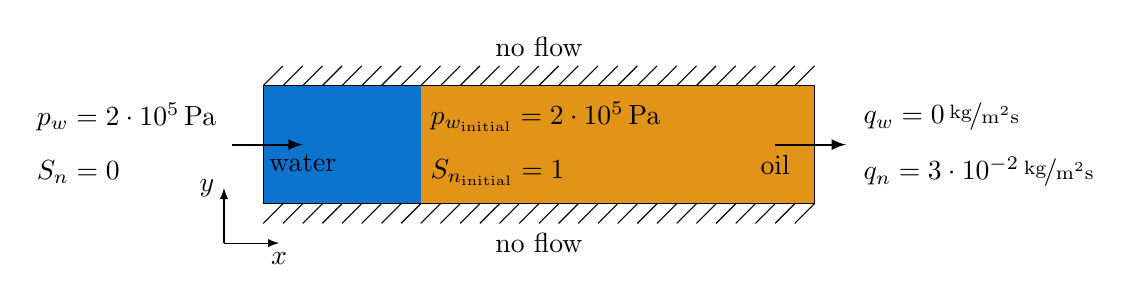
\begin{tikzpicture}[>=latex]
  % basic sketch
  \fill [fill=dumuxBlue](0,0) rectangle ++(2,1.5);
  \fill [fill=dumuxYellow](2,0) rectangle ++(5,1.5);
  \draw (0,0) rectangle ++(7,1.5);
  \foreach \x in {0,0.25,...,6.75}
    \draw (\x,1.5) -- ++(0.25,0.25);
  \foreach \x in {0,0.25,...,6.75}
    \draw (\x,-0.25) -- ++(0.25,0.25);
  % labels
  \draw [->](-0.5,-0.5) -- ++(0,0.7) node [anchor=east]{$y$};
  \draw [->](-0.5,-0.5) -- ++(0.7,0) node [anchor=north]{$x$};
  \node at(3.5,1.75)[anchor=south]{no flow};
  \node at(3.5,-0.25)[anchor=north]{no flow};
  \draw[->,thick](-0.4,0.75) -- ++(0.9,0) node[anchor=north]{water};
  \draw[->,thick](6.5,0.75)node[anchor=north]{oil} -- ++(0.9,0);
  % equations
  \node [anchor=west] at (2,1.1){$p_{w_\text{initial}} = \unit[2 \cdot 10^5]{Pa}$};
  \node [anchor=west] at (2,0.4){$S_{n_\text{initial}} = 1$};
  \node [anchor=west] at (-3,1.1){$p_w = \unit[2 \cdot 10^5]{Pa}$};
  \node [anchor=west] at (-3,0.4){$S_n = 0$};
  \node [anchor=west] at (7.5,1.1){$q_w = \unitfrac[0]{kg}{m^2s}$};
  \node [anchor=west] at (7.5,0.4){$q_n = \unitfrac[3 \cdot 10^{-2}] {kg}{m^2s}$};
\end{tikzpicture}
\caption{Geometry of the tutorial problem with initial and boundary conditions.}
\label{tutorial-coupled:problemfigure}
\end{figure}

The solved equations are the mass balances of water and oil:
\begin{align}
  \label{massbalancewater}
  \frac {\partial (\phi \, S_{w}\, \varrho_{w})}{\partial t}
  -
  \nabla \cdot \left( \varrho_{w} \, \frac{k_{rw}}{\mu_{w}} \, \mathbf{K}\;\nabla p_w \right)
  -
  q_w
  & =
  0 \\
  \label{massbalanceoil}
  \frac {\partial (\phi \, S_{o}\, \varrho_{o})}{\partial t}
  -
  \nabla \cdot \left( \varrho_{o} \, \frac{k_{ro}}{\mu_{o}} \, \mathbf{K}\;\nabla p_o \right)
  -
  q_o
  & =
  0
\end{align}

\subsection{The Main File}

Listing \ref{tutorial-coupled:mainfile} shows the main application file
\texttt{tutorial/tutorial\_coupled.cc} for the coupled two-phase
model. This file has to be compiled and executed in order to solve the problem described
above.

\begin{lst}[File tutorial/tutorial\_coupled.cc]\label{tutorial-coupled:mainfile} \mbox{}
  \lstinputlisting[style=DumuxCode, numbersep=5pt, firstline=24, firstnumber=24]{../../tutorial/tutorial_coupled.cc}
\end{lst}

From line \ref{tutorial-coupled:include-begin} to line
\ref{tutorial-coupled:include-end} the required headers are included.

At line \ref{tutorial-coupled:set-type-tag} the type tag of the
problem, which is going to be simulated, is specified. All other data
types can be retrieved via the \Dumux property system and only depend
on this single type tag. For a more thorough introduction to the
\Dumux property system, see chapter~\ref{sec:propertysystem}.

After this, the default startup routine \texttt{Dumux::start()} is
called on line \ref{tutorial-coupled:call-start}. This function deals
with parsing the command line arguments, reading the parameter file,
setting up the infrastructure necessary for \Dune, loading the grid, and
starting the simulation.
Required parameters for the start of the simulation,
such as the initial time-step size, the simulation time or details of the grid,
can be either specified by command line arguments of the form
(\texttt{-ParameterName ParameterValue}), in the file specified by the
\texttt{-ParameterFile} argument, or if the latter is not specified,
in the file \mbox{\texttt{tutorial\_coupled.input}}.
If a parameter is
specified on the command line as well as in the parameter file, the
values provided in the command line have
precedence. Listing~\ref{tutorial-coupled:parameter-file} shows the
default parameter file for the tutorial problem.

\begin{lst}[File tutorial/tutorial\_coupled.input]\label{tutorial-coupled:parameter-file} \mbox{}
\lstinputlisting[style=DumuxParameterFile]{../../tutorial/tutorial_coupled.input}
\end{lst}

To provide an error message, the usage message which is displayed to
the user if the simulation is called incorrectly, is printed via the
custom function which is defined on
line~\ref{tutorial-coupled:usage-function} in the main file.
In this function the usage message is customized to the problem at hand.
This means that at least the necessary parameters are listed here.
For more information about the input file please refer to section \ref{sec:inputFiles}.


\subsection{The Problem Class}\label{tutorial-coupled:problem}

When solving a problem using \Dumux, the most important file is the
so-called \textit{problem file} as shown in
listing~\ref{tutorial-coupled:problemfile}.

\begin{lst}[File tutorial/tutorialproblem\_coupled.hh]\label{tutorial-coupled:problemfile} \mbox{}
\lstinputlisting[style=DumuxCode, numbersep=5pt, firstline=24, firstnumber=24]{../../tutorial/tutorialproblem_coupled.hh}
\end{lst}

First, a new type tag is created for the problem in line
\ref{tutorial-coupled:create-type-tag}.  In this case, the new type
tag inherits all properties from the \texttt{BoxTwoP} type tag, which
means that for this problem the two-phase box model is chosen as
discretization scheme. Further, it inherits from the spatial
parameters type tag, which is defined in line
\ref{tutorial-coupled:define-spatialparameters-typetag} of the problem-dependent spatial
parameters file.  On line
\ref{tutorial-coupled:set-problem}, a problem class is attached to the
new type tag, while the grid which is going to be used is defined in
line \ref{tutorial-coupled:set-grid} -- in this case that is
\texttt{Dune::YaspGrid}.  Since there's no uniform mechanism to
allocate grids in \Dune, \Dumux features the concept of grid creators.
In this case the generic \texttt{CubeGridCreator} which creates a
structured hexahedron grid of a specified size and resolution. For
this grid creator the  physical domain of the grid is specified via the
run-time parameters \texttt{Grid.upperRightX},
\texttt{Grid.upperRightY}, \texttt{Grid.numberOfCellsX} and
\texttt{Grid.numberOfCellsY}. These parameters can be specified via
the command-line or in a parameter file.

Next, the appropriate fluid system, which specifies the thermodynamic
relations of the fluid phases, has to be chosen. By default, the
two-phase model uses the \texttt{TwoPImmiscibleFluidSystem}, which
assumes immiscibility of the phases, but requires the components
used for the wetting and non-wetting phases to be explicitly set. In
this case, liquid water which uses the relations from
IAPWS'97~\cite{IAPWS1997} is chosen as the wetting phase on line
\ref{tutorial-coupled:wettingPhase} and liquid oil is chosen as the
non-wetting phase on line \ref{tutorial-coupled:nonwettingPhase}. The
last property, which is set in line \ref{tutorial-coupled:gravity},
tells the model not to use gravity.

\label{tutorial-coupled:boundaryStart}Parameters which are specific to a physical set-up to be simulated,
such as boundary and initial conditions, source terms or temperature
within the domain, and which are required to solve the differential
equations of the models are specified via a \textit{problem} class. This class
should be derived from \texttt{ImplicitPorousMediaProblem} as done in line
\ref{tutorial-coupled:def-problem}.

The problem class always has at least five methods:
\begin{itemize}
\item A method \texttt{boundaryTypes()} specifying the type of
  boundary conditions at each vertex.
\item A method \texttt{dirichlet()} specifying the actual values for
  the \textsc{Dirichlet} conditions at each \textsc{Dirichlet} vertex.
\item A method \texttt{neumann()} specifying the actual values for
  the \textsc{Neumann} conditions, which are usually evaluated at the
  integration points of the \textsc{Neumann} boundary faces.
\item A method for source or sink terms called \texttt{source()}, usually evaluated at
  the center of a control volume.
\item A method called \texttt{initial()} for specifying the initial
  conditions at each vertex.
\end{itemize}

For the definition of the boundary condition types and of the
values of the \textsc{Dirichlet} boundaries, two parameters are
available:
\begin{description}
 \item [bcTypes/values:]  A vector which stores the result of the method. What
  the values in this vector mean is dependent on the method: For
  \texttt{dirichlet()}, \texttt{values} contains the actual values of the primary
  variables, for \texttt{boundaryTypes()}, \texttt{bcTypes} contains the boundary
  condition types. It has as many entries as the model has primary variables / equations.
  For the typical case, in which all equations have the same boundary
  condition type at a certain position, there are two methods that set the appropriate conditions
  for all primary variables / equations: \texttt{setAllDirichlet()} and \texttt{setAllNeumann()}.
\item [vertex:] The boundary condition and the Dirichlet values are
  specified for a vertex, which represents a sub-control volume in the box
  discretization. This inhibits the specification of two different
  boundary condition types for one equation at one sub-control
  volume.  Be aware that the second parameter is a Dune grid entity
  with the codimension \texttt{dim}.
\end{description}

To ensure that no boundaries are undefined, a small safeguard value
\texttt{eps\_} is usually added when comparing spatial
coordinates. The left boundary is hence not detected by checking, if the
first coordinate of the global position is equal to zero, but by testing whether it is
smaller than a very small value \texttt{eps\_}.

Methods for box models which make statements about boundary segments of the grid
(such as \texttt{neumann()}) are called with six arguments:
\begin{description}
\item[values:] A vector \texttt{neumann()}, in which the mass fluxes per area unit
  over the boundary segment are specified.
\item[element:] The element of the grid where the boundary segment
  is located.
\item[fvGeometry:] The finite-volume geometry induced on the
  finite element by the box scheme.
\item[intersection:] The \texttt{Intersection} of the boundary segment as given by the grid.
\item[scvIdx:] The index of the sub-control volume in
  \texttt{fvGeometry} which is assigned to the boundary segment.
\item[boundaryFaceIdx:] The index of the boundary face in
  \texttt{fvGeometry} which represents the boundary segment.
\end{description}

Similarly, the \texttt{initial()} and \texttt{source()} methods
specify properties of control volumes and thus only get
\texttt{values}, \texttt{element}, \texttt{fvGeometry} and
\texttt{scvIdx} as arguments.

In addition to these five methods, there might be some model-specific
methods. If the isothermal two-phase model is used, this includes for
example a \texttt{temperature()} method which returns the temperature
in \textsc{Kelvin} of the fluids and the rock matrix in the
domain. This temperature is then used by the model to calculate fluid
properties which possibly depend on it, e.g. density. The
\texttt{bBoxMax()} (``\textit{max}imum coordinated of the grid's
\textit{b}ounding \textit{box}'') method is used here to
determine the extend of the physical domain. It returns a vector with the
maximum values of each global coordinate of the grid. This method
and the analogous \texttt{bBoxMin()} method are provided by the base
class \texttt{Dumux::BoxProblem<TypeTag>}.

\subsection{Defining Fluid Properties}\label{tutorial-coupled:description-fluid-class}

The \Dumux distribution includes some common substances which can be
used out of the box. The properties of the pure substances (such as
the components nitrogen, water, or the pseudo-component air) are
provided by header files located in the folder
\verb+dumux/material/components+.

Most often, when two or more components are considered, fluid
interactions such as solubility effects come into play and properties
of mixtures such as density or enthalpy are of interest. These
interactions are defined by {\em fluid systems}, which are located in
\verb+dumux/material/fluidsystems+. A more thorough overview of the
\Dumux fluid framework can be found in chapter~\ref{sec:fluidframework}.

% In this example, a class for the definition of a two-phase system is used. This allows for the choice
% of the two components oil and water and for access of the parameters that are relevant for the two-phase model.

\subsection{Defining Spatially Dependent Parameters}\label{tutorial-coupled:description-spatialParameters}

In \Dumux, many properties of the porous medium can depend on the
spatial location. Such properties are the \textit{intrinsic
  permeability}, the parameters of the \textit{capillary pressure} and
the \textit{relative permeability}, the \textit{porosity}, the
\textit{heat capacity} as well as the \textit{heat conductivity}. Such
parameters are defined using a so-called \textit{spatial parameters}
class.

If the box discretization is used, the spatial parameters class
should be derived from the base class
\texttt{Dumux::BoxSpatialParams<TypeTag>}. Listing
\ref{tutorial-coupled:spatialparametersfile} shows the file \\
\verb+tutorialspatialparams_coupled.hh+:

\begin{lst}[File tutorial/tutorialspatialparams\_coupled.hh]\label{tutorial-coupled:spatialparametersfile} \mbox{}
\lstinputlisting[style=DumuxCode, numbersep=5pt, firstline=25, firstnumber=25]{../../tutorial/tutorialspatialparams_coupled.hh}
\end{lst}

First, the spatial parameters type tag is created on line
\ref{tutorial-coupled:define-spatialparameters-typetag}. The type tag
for the problem is then derived from it. The \Dumux properties defined on
the type tag for the spatial parameters are, for example, the spatial
parameters class itself (line
\ref{tutorial-coupled:set-spatialparameters}) or the capillary
pressure/relative permeability relations\footnote{Taken together, the
  capillary pressure and the relative permeability relations are
  called \textit{material law}.} which ought to be used by the
simulation (line
\ref{tutorial-coupled:rawlaw} \label{tutorial-coupled:materialLaw}).
\Dumux provides several material laws in the folder
\verb+dumux/material/fluidmatrixinteractions+.  The selected one --
here it is a relation according to a regularized version of
\textsc{Brooks} \& \textsc{Corey} -- is included in line
\ref{tutorial-coupled:rawLawInclude}.
After the selection, an adapter class is specified in line \ref{tutorial-coupled:eff2abs} to
translate between effective and absolute saturations. Like this,
residual saturations can be specified in a generic way.  As only the employed
material law knows the names of the parameters which it
requires, it provides a parameter class
\texttt{RegularizedBrooksCoreyParams} which has the type
\texttt{Params} and which is defined in line
\ref{tutorial-coupled:matLawObjectType}. In this case, the spatial
parameters only require a single set of parameters which means that it
only requires a single material parameter object as can be seen in
line~\ref{tutorial-coupled:matParamsObject}.

In line \ref{tutorial-coupled:permeability}, a method returning the
intrinsic permeability is specified. As can be seen, the method has
to be called with three arguments:
\begin{description}
\item[\texttt{element}:] Just like for the problem itself, this
  parameter describes the considered element by means of a \Dune
  entity. Elements provide information about their geometry and
  position and can be mapped to a global index.
\item[\texttt{fvGeometry}:] It holds information about the finite-volume
  geometry of the element induced by the box method.
\item[\texttt{scvIdx}:] This is the index of the sub-control volume of the
  element which is considered. It is equivalent to the local index
  of the vertex which corresponds to the considered control volume in
  the element.
\end{description}

The intrinsic permeability is usually a tensor. Thus the method returns
a $\texttt{dim} \times \texttt{dim}$-matrix, where \texttt{dim} is the
dimension of the grid.

The method \texttt{porosity()} defined in line
\ref{tutorial-coupled:porosity} is called with the same arguments as
\texttt{intrinsicPermeability()} and returns a scalar value for
porosity dependent on the position in the domain.

Next, the method \texttt{materialLawParams()}, defined in line
\ref{tutorial-coupled:matLawParams}, returns the
\verb+materialParams_+ object that is applied at the specified
position. Although in this case only one object is returned, in
general, the problem may be heterogeneous, which necessitates
returning different objects at different positions in space.  While
the selection of the type of this object was already explained (line
\ref{tutorial-coupled:rawLawInclude}), some specific parameter values
of the used material law, such as the \textsc{Brooks} \&
\textsc{Corey} parameters, are still needed. This is done in the
constructor at line \ref{tutorial-coupled:setLawParams}.  Depending on
the type of the \texttt{materialLaw} object, the \texttt{set}-methods
might be different than those given in this example. The name of the
access / set functions as well as the rest of the implementation of
the material description can be found in
\verb+dumux/material/fluidmatrixinteractions/2p+.

\subsection{Exercises}
\label{tutorial-coupled:exercises}
The following exercises will give you the opportunity to learn how you
can change soil parameters, boundary conditions, run-time parameters
and fluid properties in \Dumux. Possible solutions to these exercises are given in the tutorial folder in the
sub-folder \texttt{solutions\_coupled} as \texttt{.diff} files. In these files only
the lines that are different from the original file are listed.
They can be opened using the program \texttt{kompare}, simply type \texttt{kompare SOLUTIONFILE} into the terminal.

\subsubsection{Exercise 1}
\renewcommand{\labelenumi}{\alph{enumi})} For Exercise 1 you have
to make only some small changes in the tutorial files.

\begin{enumerate}

\item \textbf{Running the Program} \\
To get an impression what the results should look like you can compile and run the original version of
the coupled tutorial model by typing \texttt{make tutorial\_coupled} followed by \texttt{./tutorial\_coupled}.
Note, that the time-step size is automatically adapted during the simulation.
For the visualization of the results using ParaView, please refer to section \ref{quick-start-guide}.

\item \textbf{Changing the Model Domain and the Boundary Conditions} \\
  Change the size of the model domain so that you get a rectangle with
  edge lengths of $\text{x} = \unit[400]{m}$ and $\text{y} = \unit[500]{m}$ and with
  discretization lengths of $\Delta \text{x} = \unit[20]{m}$ and $\Delta
  \text{y} = \unit[20]{m}$. For this you have to edit the parameter file (\texttt{tutorialproblem\_coupled.input})
  and run the program again.\\
  Note, that you do not have to recompile the program if you make changes to the parameter file.


  Change the boundary conditions in the file
  \texttt{tutorialproblem\_coupled.hh} so that water enters from the
  bottom and oil is extracted from the top boundary. The right and the
  left boundary should be closed for water and oil fluxes. \\
  The Neumannn Boundary conditions are multiplied by the normal (pointing outwards),
  so an influx is negative, an outflux always positive.
  Such information can easily be found in the documentation of the functions (also look into base classes).
  Compile the main file by typing \texttt{make tutorial\_coupled} and
  run the model as explained above.

  \item \textbf{Changing  the Shape of the Discrete Elements} \\
  In order to complete this exercise you need an external grid manager capable of handling
  simplex grids, like \texttt{ALUGrid} or \texttt{UGGrid}. If this is not the case,
  please skip this exercise.
  Change the types of elements used for discretizing the domain. In line
  \ref{tutorial-coupled:set-gridcreator} of the problem
  file  the type of gridcreator is chosen. By choosing a different grid creator
  you can discretize the domain with different elements.
  Hint: You can find gridcreators in \texttt{dumux/io/}, change for example from
  \texttt{cubegridcreator.hh} to \texttt{simplexgridcreator.hh}.
  For ALUGrid you have to change the ALUGrid type in line \ref{tutorial-coupled:set-grid-ALU} from \texttt{Dune::cube}
  to \texttt{Dune::simplex}.
  The shape of the employed elements can be visualized in ParaView by choosing \texttt{Surface with Edges}.

\item \textbf{Changing Fluids} \\
Now you can change the fluids. Use DNAPL instead of Oil and Brine instead of Water.
To do that, you have to select different components via the property system in the problem file:
\begin{enumerate}
 \item Brine: Brine is thermodynamically very similar to pure water but also
 considers a fixed amount of salt in the liquid phase.
  Hence, the class \texttt{Dumux::Brine} uses a pure water class, such as \texttt{Dumux::H2O<Scalar>},
  as a second template argument after the data type \texttt{<Scalar>}, i.e.
  \texttt{Dumux::Brine<Scalar, Dumux::H2O<Scalar>>}. The file is located in the folder \texttt{dumux/material/components/}.
  Try to include the file and select the component as the wetting phase via the property system.
 \item DNAPL:
  Now let's include a DNAPL (\textbf{d}ense \textbf{n}on-\textbf{a}queous \textbf{p}hase \textbf{l}iquid)
  which is located in the folder \texttt{dumux/material/components/}. Try to
  include the file and select the component as the non-wetting phase via the property system.
\end{enumerate}
If you want to take a closer look on how the fluid classes are defined and which
substances are already available please browse through the files in the directory
\texttt{/dumux/material/components} and read chapter~\ref{sec:fluidframework}.

\item \textbf{Use a Full-Fledged Fluid System} \\
\Dumux usually describes fluid mixtures via \textit{fluid systems}, see also chapter \ref{sec:fluidframework}.
In order to include a fluid system, you first have to comment out lines \ref{tutorial-coupled:2p-system-start}
to \ref{tutorial-coupled:2p-system-end} in the problem file. If you use eclipse,
this can easily be done by pressing \textit{Ctrl + Shift + 7} --
the same as to cancel the comment later on.\\
Now include the file \texttt{fluidsystems/h2oairfluidsystem.hh} in the material
folder, and set a type property \texttt{FluidSystem} (see line \ref{tutorial-coupled:set-fluidsystem})
with the appropriate type, which is either:\\
 \texttt{Dumux::FluidSystems::H2OAir<typename GET\_PROP\_TYPE(TypeTag, Scalar)>}\\
or in the \Dumux tongue\\
 \texttt{Dumux::H2OAirFluidSystem<TypeTag>}
\\
However, this is a rather complicated fluid system which
considers mixtures of components and also uses tabulated components that need to
be initialized -- i.e. the tables need to be filled with values.
The initialization of the fluid system is normally done in the constructor of the
problem by calling \texttt{GET\_PROP\_TYPE(TypeTag, FluidSystem)::init();}.
Remember that the constructor function always has the same name as the respective
class, i.e. \texttt{TutorialProblemCoupled(..)}.\\
As water flow replacing a gas is much faster, test your simulation only until $2000$
seconds and start with a time-step of $1$ second.\\
Please reverse the changes made in this part of the exercise, as we will continue
to use immiscible phases from here on and hence do not need a complex fluid system.

\item \textbf{Changing Constitutive Relations} \\
  Use an unregularized linear law with an entry pressure of $p_e = \unit[0.0]{Pa}$
  and maximal capillary pressure of e.g. $p_{c_{max}} = \unit[2000.0]{Pa}$ instead of using a
 regularized Brooks-Corey law for the
  relative permeability and for the capillary pressure saturation relationship.
  To do that you have
  to change the material law property (line \ref{tutorial-coupled:eff2abs}) in
  \texttt{tutorialspatialparams\_coupled.hh}. Leave the type definition of \texttt{Scalar} and remove
 the type definition of \texttt{BrooksAndCorey} in the private section of
 the property definition. Exchange the \texttt{EffToAbsLaw} with the \texttt{LinearMaterial} law type in the
public section.
 You can find the material laws in the folder
  \verb+dumux/material/fluidmatrixinteractions+. The necessary parameters
of the linear law and the respective \texttt{set}-functions can be found
 in the file \\
 \verb+dumux/material/fluidmatrixinteractions/2p/linearmaterialparams.hh+.\\
Call the \texttt{set}-functions from the constructor of the \texttt{tutorialspatialparams\_coupled.hh}.

\item \textbf{Heterogeneities}  \\
  Set up a model domain with the soil properties given in Figure
  \ref{tutorial-coupled:exercise1_d}. Adjust the boundary conditions
  so that water is again flowing from the left to the right of the
\begin{figure}[ht]
\centering
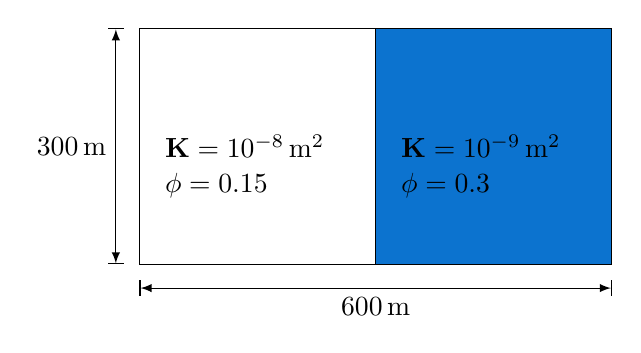
\begin{tikzpicture}[>=latex]
  % basic sketch
  \fill [dumuxBlue](3,0) rectangle ++(3,3);
  \draw (3,0) -- ++(0,3);
  \draw (0,0) rectangle ++(6,3);
  % arrows
  \draw [|<->|](0,-0.3) -- ++(6,0);
  \node at (3,-0.3)[anchor=north]{$\unit[600]{m}$};
  \draw [|<->|](-0.3,0) -- ++(0,3);
  \node at(-0.3,1.5)[anchor=east]{$\unit[300]{m}$};
  % labels
  \node [anchor=west] at (0.2,1.5){$\mathbf{K}=\unit[10^{-8}]{m^2}$};
  \node [anchor=west] at (0.2,1){$\phi=0.15$};
  \node [anchor=west] at (3.2,1.5){$\mathbf{K}=\unit[10^{-9}]{m^2}$};
  \node [anchor=west] at (3.2,1){$\phi=0.3$};
\end{tikzpicture}
\caption{Exercise 1g: Set-up of a model domain with a heterogeneity. Grid
spacing: $\Delta x = \unit[20]{m}$ $\Delta y = \unit[20]{m}$.}\label{tutorial-coupled:exercise1_d}
\end{figure}
domain. You can use the fluids of exercise 1b.\\
\textbf{Hint:} The current position of the control volume can be obtained
using \texttt{element\allowbreak.geometry()\allowbreak.corner(scvIdx)}, which
returns a vector of the global coordinates of the current position.\\
When does the front cross the material border? In ParaView, the
animation view (\textit{View} $\rightarrow$ \textit{Animation
  View}) is a convenient way to get a rough feeling of the time-step
sizes.
\end{enumerate}

\subsubsection{Exercise 2}
For this exercise you should create a new problem file analogous to
the file \texttt{tutorialproblem\_coupled.hh} (e.g. with the name
\texttt{ex2\_tutorialproblem\_coupled.hh} and new spatial parameters \texttt{ex2\_tutorialspatialparams\_coupled.hh},
just like \texttt{tutorialspatialparams\_coupled.hh}.

The new files should contain the definition of new classes with names
that relate to the file name, such as
\texttt{Ex2TutorialProblemCoupled}. Make sure that you also adjust the
guardian macros in lines \ref{tutorial-coupled:guardian1} and
\ref{tutorial-coupled:guardian2}
in the header files (e.g. change
\mbox{\texttt{DUMUX\_TUTORIALPROBLEM\_COUPLED\_HH}} to\\
\mbox{\texttt{DUMUX\_EX2\_TUTORIALPROBLEM\_COUPLED\_HH}}). Include the new problem file in \texttt{tutorial\_coupled.cc}.
Besides adjusting the guardian macros, the new problem file should define and
use a new type tag for the problem as well as a new problem class
e.g. \mbox{\texttt{Ex2TutorialProblemCoupled}}. The type tag definition has
to be adjusted in \texttt{tutorial\_coupled.cc} too (see line \ref{tutorial-coupled:set-type-tag}).
Similarly adjust your new spatial parameters file. If you are using Eclipse there is
a very helpful function called \texttt{Refactor} which you can use to change
all similar variables or types in your current file in one go. Just place the
cursor at the variable or type you want to change
and use the \texttt{Refactor} $\rightarrow$ \texttt{Rename} functionality. Make sure to assign your
newly defined spatial parameter class to the
\texttt{SpatialParams} property for the new
type tag.

After this, change the run-time parameters so that they match the
domain described by figure \ref{tutorial-coupled:ex2_Domain}. Adapt
the problem class so that the boundary conditions are consistent with
figure \ref{tutorial-coupled:ex2_BC}. Initially, the domain is fully
saturated with water and the pressure is $p_w = \unit[5 \times
10^5]{Pa}$. Oil infiltrates from the left side. Create a grid
with $20$ cells in $x$-direction and $10$ cells in $y$-direction. The
simulation time should be set to $\unit[10^6]{s}$ with an
initial time-step size of $\unit[100]{s}$. Then, you can compile the program.


\begin{figure}[ht]
\centering
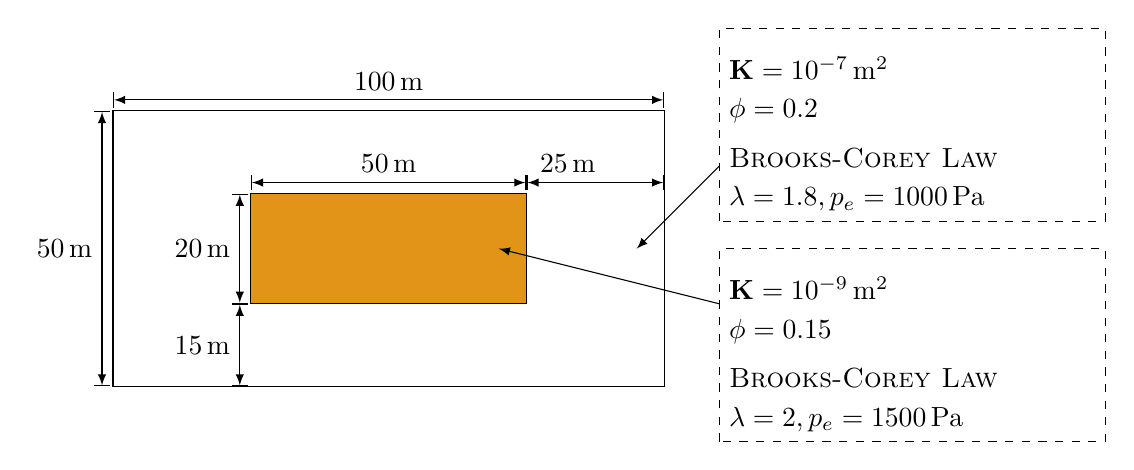
\begin{tikzpicture}[scale=0.7,>=latex]
  % basic sketch
  \draw (0,0) rectangle ++(10,5);
  \draw [fill=dumuxYellow] (2.5,1.5) rectangle ++(5,2);
  % arrows
  \draw[|<->|] (-0.2,0) -- ++(0,5);
  \node [anchor=east] at (-0.2,2.5){$\unit[50]{m}$};
  \draw[|<->|] (0,5.2) -- ++(10,0);
  \node [anchor=south] at (5,5.2){$\unit[100]{m}$};
  \draw[|<->|] (2.3,1.5) -- ++(0,2);
  \node [anchor=east] at (2.3,2.5){$\unit[20]{m}$};
  \draw[|<->|] (2.3,0) -- ++(0,1.5);
  \node [anchor=east] at (2.3,0.75){$\unit[15]{m}$};
  \draw[|<->|] (2.5,3.7) -- ++(5,0);
  \node [anchor=south] at (5,3.7){$\unit[50]{m}$};
  \draw[|<->|] (7.5,3.7) -- ++(2.5,0);
  \node [anchor=south] at (8.25,3.7){$\unit[25]{m}$};
  % labels
  \draw [dashed] (11,3) rectangle ++(7,3.5);
  \node [anchor=south west] at (11,5.4){$\mathbf{K} = \unit[10^{-7}]{m^2}$};
  \node [anchor=south west] at (11,4.6){$\phi = 0.2$};
  \node [anchor=south west] at (11,3.8){\textsc{Brooks-Corey Law}};
  \node [anchor=south west] at (11,3.0){$\lambda = 1.8, p_e = \unit[1000]{Pa}$};
  \draw [->] (11,4) -- (9.5,2.5);
  \draw [dashed] (11,-1) rectangle ++(7,3.5);
  \node [anchor=south west] at (11,1.4){$\mathbf{K} = \unit[10^{-9}]{m^2}$};
  \node [anchor=south west] at (11,0.6){$\phi = 0.15$};
  \node [anchor=south west] at (11,-0.2){\textsc{Brooks-Corey Law}};
  \node [anchor=south west] at (11,-1.0){$\lambda = 2, p_e = \unit[1500]{Pa}$};
  \draw [->] (11,1.5) -- (7,2.5);
\end{tikzpicture}
\caption{Set-up of the model domain and the soil parameters}\label{tutorial-coupled:ex2_Domain}
\end{figure}

\begin{figure}[ht]
\centering
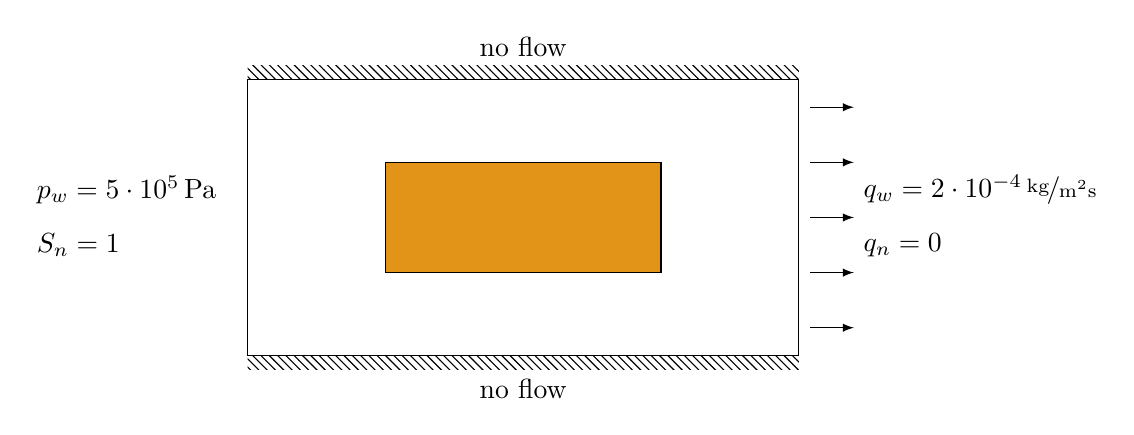
\begin{tikzpicture}[scale=0.7,>=latex]
  % basic sketch
  \fill [pattern=north west lines] (0,0) rectangle ++(10,-0.25);
  \fill [pattern=north west lines] (0,5) rectangle ++(10,0.25);
  \draw (0,0) rectangle ++(10,5);
  \draw [fill=dumuxYellow] (2.5,1.5) rectangle ++(5,2);
  \foreach \y in {0.5,1.5,...,4.5}
    \draw [->](10.2,\y) -- ++(0.8,0);
  % labels
  \node [anchor=south] at (5,5.25){no flow};
  \node [anchor=north] at (5,-0.25){no flow};
  \node [anchor=west] at(11,2){$q_n = 0$};
  \node [anchor=west] at(11,3){$q_w = \unitfrac[2 \cdot 10^{-4}]{kg}{m^2 s}$};
  \node [anchor=west] at(-4,2){$S_n = 1$};
  \node [anchor=west] at(-4,3){$p_w = \unit[5 \cdot 10^5]{Pa}$};
\end{tikzpicture}
\caption{Boundary Conditions}\label{tutorial-coupled:ex2_BC}
\end{figure}

\begin{itemize}
 \item Increase the simulation time to e.g. $\unit[4\times 10^7]{s}$. Investigate the saturation: Is the value range reasonable?
 \item What happens if you increase the resolution of the grid?
\end{itemize}

\subsubsection{Exercise 3: Parameter File Input}

As you have experienced, compilation takes quite some time. Therefore,
\Dumux provides a simple method to read in parameters at run-time
via \textit{parameter input files}.

In the code, parameters can be read via the macro
\texttt{GET\_RUNTIME\_PARAM(TypeTag, Scalar,
MyWonderfulGroup.MyWonderfulParameter);}. In this exercise we will explore the possibilities of the
parameter file. For this we take a look at the file \texttt{ex3\_tutorial\_coupled.input} in the \texttt{solutions\_coupled} folder.
Besides the parameters which you already used in the parameter file above,
there are parameters which can be used to control the
Newton and the Linear solver (groups: \texttt{Newton} and \texttt{LinearSolver}).
Run-time parameters used in the problem or spatial parameters classes
can also be set with the respective group names (\texttt{Problem} and \texttt{SpatialParams})
in the parameter file. For the latter parameters to be included in the program
they have to be assigned in the problem or spatial parameters constructor. This
can be done as shown in the files \texttt{ex3\_tutorialproblem\_coupled.diff}
and \texttt{ex3\_tutorialspatialparams\_coupled.diff} in the \texttt{solutions\_coupled} folder. Add some (for
example \texttt{Newton.MaxSteps} and \texttt{Problem.EnableGravity}) to the
parameter file \texttt{tutorial\_coupled.input} and observe what
happens if they are modified. For more information about the input file please refer to section \ref{sec:inputFiles}.

\subsubsection{Exercise 4: Create a New Component}

Create a new file for the benzene component called \texttt{benzene.hh}
and implement a new component. (You may get a hint by looking at
existing components in the directory \verb+/dumux/material/components+). \\
Use benzene as a new fluid and run the model of Exercise 2 with water
and benzene. Benzene has a density of $\unitfrac[889.51]{kg}{m^3}$ and
a viscosity of $\unit[0.00112]{Pa \, s}$.


\subsubsection{Exercise 5: Time Dependent Boundary Conditions}

In this exercise we want to investigate the influence of time dependent boundary
conditions. For this, redo the steps of exercise 2 and create a new problem and
spatial parameters file.

After this, change the run-time parameters so that they match the
domain described by figure \ref{tutorial-coupled:ex5_Domain}. Adapt
the problem class so that the boundary conditions are consistent with
figure \ref{tutorial-coupled:ex5_BC}. Here you can see the time dependence of the
nonwetting saturation, where water infiltrates only during $\unit[10^5]{s}$ and
$\unit[4 \cdot 10^5]{s}$. To implement these time dependencies you need the actual
time $t_{n+1}=t_n + \Delta t$ and the endtime of the simulation. For this you can
use the methods \texttt{this->timeManager().time()}, \texttt{this->timeManager().timeStepSize()}
and \texttt{this->timeManager().endTime()}.

Initially, the domain is fully saturated with oil and the pressure is $p_w = 2 \times
10^5\,\text{Pa}$.  Water infiltrates from the left side. Create a grid
with $100$ cells in $x$-direction and $10$ cells in $y$-direction. The
simulation time should be set to $\unit[5 \cdot 10^5]{s}$ with an
initial time-step size of $\unit[10]{s}$. To avoid too big time-step sizes
you should set the parameter \texttt{MaxTimeStepSize} for the group \texttt{TimeManager}
(in your input file) to $\unit[1000]{s}$.  Then, you can compile the program.

\begin{figure}[ht]
\centering
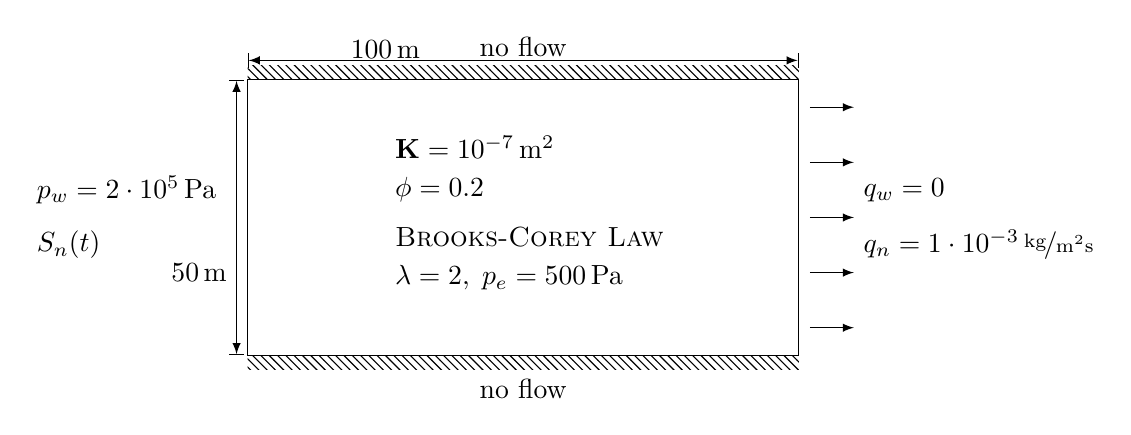
\begin{tikzpicture}[scale=0.7,>=latex]
  % basic sketch
  \fill [pattern=north west lines] (0,0) rectangle ++(10,-0.25);
  \fill [pattern=north west lines] (0,5) rectangle ++(10,0.25);
  \draw (0,0) rectangle ++(10,5);
  \foreach \y in {0.5,1.5,...,4.5}
    \draw [->](10.2,\y) -- ++(0.8,0);
  % arrows
  \draw[|<->|] (-0.2,0) -- ++(0,5);
  \node [anchor=east] at (-0.2,1.5){$\unit[50]{m}$};
  \draw[|<->|] (0,5.35) -- ++(10,0);
  \node [anchor=south] at (2.5,5.2){$\unit[100]{m}$};
  % labels
  \node [anchor=south] at (5,5.25){no flow};
  \node [anchor=north] at (5,-0.25){no flow};
  \node [anchor=west] at(11,2){$q_n = \unitfrac[1 \cdot 10^{-3}]{kg}{m^2 s}$};
  \node [anchor=west] at(11,3){$q_w = 0$};
  \node [anchor=west] at(-4,2){$S_n(t)$};
  \node [anchor=west] at(-4,3){$p_w = \unit[2 \cdot 10^5]{Pa}$};
  \node [anchor=south west] at (2.5,3.4){$\mathbf{K} = \unit[10^{-7}]{m^2}$};
  \node [anchor=south west] at (2.5,2.6){$\phi = 0.2$};
  \node [anchor=south west] at (2.5,1.8){\textsc{Brooks-Corey Law}};
  \node [anchor=south west] at (2.5,1.0){$\lambda = 2, \; p_e = \unit[500]{Pa}$};
\end{tikzpicture}
\caption{Set-up of the model domain and the soil parameters}\label{tutorial-coupled:ex5_Domain}
\end{figure}

\begin{figure}[ht]
\centering
\begin{tikzpicture}[scale=0.9,>=latex]
    % Draw axes
    \draw [<->,thick] (0,6) node (yaxis) [above] {$S_n$}
        |- (11,0) node (xaxis) [right] {time\,[s]};
    \draw plot[smooth,samples=100,domain=0:1] (6*\x + 2 ,{5*sin((\x+1)*pi r)+5});
	\draw [-] (0,5) -- (2,5);
	\draw [-] (8,5) -- (10,5);
    \draw [dashed] (2,5) -- (2,0);
    \draw [dashed] (8,5) -- (8,0);
    \draw [dashed] (10,5) -- (10,0);

    % axes labeling
    \draw [-] (-0.1,5) -- (0.1,5);
    \node [anchor=west] at(-0.5,5){$1$};
    \draw [-] (-0.1,0) -- (0.1,0);
    \node [anchor=west] at(-0.5,0){$0$};
    \draw [-] (2,0.1) -- (2,-0.1);
    \node [anchor=west] at(1.5,-0.4){$1\cdot10^{5}$};
    \draw [-] (8,0.1) -- (8,-0.1);
    \node [anchor=west] at(7.5,-0.4){$4\cdot10^{5}$};
    \draw [-] (10,0.1) -- (10,-0.1);
    \node [anchor=west] at(9.5,-0.4){$5\cdot10^{5}$};

    \node [anchor=base] at (5,3){$1-\sin\left(\pi\frac{\text{time}-10^5}{3\cdot 10^5 }\right)$};
\end{tikzpicture}
\caption{Time Dependent Boundary Conditions}\label{tutorial-coupled:ex5_BC}
\end{figure}

\begin{itemize}
 \item Open ParaView and plot the values of $S_n$ at time $\unit[5 \cdot 10^5]{s}$
 over the $x$-axis.\\ (\texttt{Filter->Data Analysis->Plot Over Line})
 \item What happens without any time-step restriction?
\end{itemize}

\clearpage \newpage
%%% Local Variables:
%%% mode: latex
%%% TeX-master: "dumux-handbook"
%%% End:

\section[Decoupled model]{Solving a problem using a Decoupled Model}\label{tutorial-decoupled}
The process of solving a problem using \Dumux can be roughly divided into four parts:
\begin{enumerate}
 \item The geometry of the problem and correspondingly a grid have to be defined.
 \item Material properties and constitutive relationships have to be defined.
 \item Boundary conditions as well as initial conditions have to be defined.
 \item A suitable model has to be chosen.
\end{enumerate}

In contrast to the last section, we now apply a decoupled solution procedure, a
so-called \textit{IMPET} (\textit{IM}plicit \textit{P}ressure \textit{E}xplicit
\textit{T}ransport) algorithm. This means that the pressure equation is first
solved using an implicit method. The resulting velocities are then used to solve
a transport equation explicitly.\\
In this tutorial, pure fluid phases are solved with a finite volume discretization
of both pressure- and transport step. Primary variables, according to default
settings of the model, are the pressure and the saturation of the wetting phase.

The problem which is solved in this tutorial is illustrated in figure
\ref{tutorial-decoupled:problemfigure}. A rectangular domain with no flow
boundaries on the top and at the bottom, which is initially saturated with oil,
is considered. Water infiltrates from the left side into the domain. Gravity
effects are neglected.

\begin{figure}[ht]
\centering
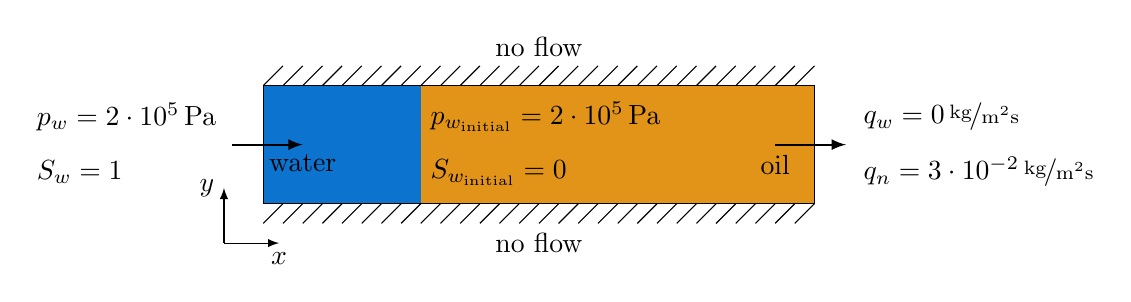
\begin{tikzpicture}[>=latex]
  % basic sketch
  \fill [fill=dumuxBlue](0,0) rectangle ++(2,1.5);
  \fill [fill=dumuxYellow](2,0) rectangle ++(5,1.5);
  \draw (0,0) rectangle ++(7,1.5);
  \foreach \x in {0,0.25,...,6.75}
    \draw (\x,1.5) -- ++(0.25,0.25);
  \foreach \x in {0,0.25,...,6.75}
    \draw (\x,-0.25) -- ++(0.25,0.25);
  % labels
  \draw [->](-0.5,-0.5) -- ++(0,0.7) node [anchor=east]{$y$};
  \draw [->](-0.5,-0.5) -- ++(0.7,0) node [anchor=north]{$x$};
  \node at(3.5,1.75)[anchor=south]{no flow};
  \node at(3.5,-0.25)[anchor=north]{no flow};
  \draw[->,thick](-0.4,0.75) -- ++(0.9,0) node[anchor=north]{water};
  \draw[->,thick](6.5,0.75)node[anchor=north]{oil} -- ++(0.9,0);
  % equations
  \node [anchor=west] at (2,1.1){$p_{w_\text{initial}} = \unit[2 \cdot 10^5]{Pa}$};
  \node [anchor=west] at (2,0.4){$S_{w_\text{initial}} = 0$};
  \node [anchor=west] at (-3,1.1){$p_w = \unit[2 \cdot 10^5]{Pa}$};
  \node [anchor=west] at (-3,0.4){$S_w = 1$};
  \node [anchor=west] at (7.5,1.1){$q_w = \unitfrac[0]{kg}{m^2s}$};
  \node [anchor=west] at (7.5,0.4){$q_n = \unitfrac[3 \cdot 10^{-2}] {kg}{m^2s}$};
\end{tikzpicture}
\caption{Geometry of the tutorial problem with initial and boundary conditions.}
\label{tutorial-decoupled:problemfigure}
\end{figure}

Listing \ref{tutorial-decoupled:mainfile} shows how the main file, which has to be
executed, has to be set up, if the problem described above is to be solved using
a decoupled model. This main file can be found in the directory \texttt{/tutorial}
of the stable part of \Dumux.

\begin{lst}[File tutorial/tutorial\_decoupled.cc]\label{tutorial-decoupled:mainfile} \mbox{}
\lstinputlisting[style=DumuxCode, numbersep=5pt, firstline=24, firstnumber=24]{../../tutorial/tutorial_decoupled.cc}
\end{lst}

First, from line \ref{tutorial-decoupled:include-begin} to line
\ref{tutorial-decoupled:include-end} the \Dune and \Dumux files containing
essential functions and classes are included.

At line \ref{tutorial-decoupled:set-type-tag} the type tag of the
problem which is going to be simulated is set. All other data types
can be retrieved by the \Dumux property system and only depend on this
single type tag. For an introduction to the
property system, see section \ref{sec:propertysystem}.

After this \Dumux' default startup routine \texttt{Dumux::start()} is
called in line \ref{tutorial-decoupled:call-start}. This function deals
with parsing the command line arguments, reading the parameter file,
setting up the infrastructure necessary for \Dune, loading the grid, and
starting the simulation. All parameters can
be either specified by command line arguments of the form
(\texttt{-ParameterName ParameterValue}), in the file specified by the
\texttt{-parameterFile} argument, or if the latter is not specified,
in the file \texttt{tutorial\_decoupled.input}. If a parameter is
specified on the command line as well as in the parameter file, the
values provided in the command line have
precedence. Listing~\ref{tutorial-decoupled:parameter-file} shows the
default parameter file for the tutorial problem.

\begin{lst}[File tutorial/tutorial\_decoupled.input]\label{tutorial-decoupled:parameter-file} \mbox{}
\lstinputlisting[style=DumuxParameterFile]{../../tutorial/tutorial_decoupled.input}
\end{lst}

To provide an error message, the usage message which is displayed to
the user if the simulation is called incorrectly, is printed via the
custom function which is defined on
line~\ref{tutorial-decoupled:usage-function}. In this function the usage
message is customized to the problem at hand. This means that at least
the necessary parameters are listed here.

\subsection{The Problem Class}
\label{decoupled_problem}

When solving a problem using \Dumux, the most important file is the
so-called \textit{problem file} as shown in listing
\ref{tutorial-decoupled:problemfile} of
\texttt{tutorialproblem\_decoupled.hh}.

\begin{lst}[File tutorial/tutorialproblem\_decoupled.hh]\label{tutorial-decoupled:problemfile} \mbox{}
\lstinputlisting[style=DumuxCode, numbersep=5pt, firstline=24, firstnumber=24]{../../tutorial/tutorialproblem_decoupled.hh}
\end{lst}

First, both \Dune  grid handlers and the decoupled model of \Dumux
have to be included. Then, a new type tag is created for the problem
in line \ref{tutorial-decoupled:create-type-tag}.  In this case, the
new type tag inherits all properties defined for the \texttt{DecoupledTwoP}
type tag, which means that for this problem the two-phase decoupled approach
is chosen as discretization scheme (defined via the include in line
\ref{tutorial-decoupled:parent-problem}). On line \ref{tutorial-decoupled:set-problem},
a problem class is attached to the new type tag, while the grid which
is going to be used is defined in line \ref{tutorial-decoupled:set-grid-type} --
in this case an \texttt{YaspGrid} is created. Since there's no uniform mechanism to
allocate grids in \Dune, \Dumux features the concept of grid creators.
In this case the generic \texttt{CubeGridCreator} (line \ref{tutorial-decoupled:set-gridcreator}) which creates a
structured hexahedron grid of a specified size and resolution. For
this grid creator the  physical domain of the grid is specified via the
run-time parameters \texttt{Grid.upperRightX},
\texttt{Grid.upperRightY}, \texttt{Grid.numberOfCellsX} and
\texttt{Grid.numberOfCellsY}. These parameters can be specified via
the command-line or in a parameter file.
For more information about the \Dune grid interface, the different grid types
that are supported and the generation of different grids consult
the \textit{Dune Grid Interface HOWTO} \cite{DUNE-HP}.

Next, we select the material of the simulation: In the case of a pure two-phase
model, each phase is a bulk fluid, and the complex (compositional) fluidsystems
do not need to be used. However, they can be used (see exercise 1 \ref{dec-ex1-fluidsystem}).
Instead, we use a simplified fluidsystem container that provides classes
for liquid and gas phases, line \ref{tutorial-decoupled:2p-system-start} to
\ref{tutorial-decoupled:2p-system-end}. These are linked to the appropriate
chemical species in line \ref{tutorial-decoupled:wettingPhase} and
\ref{tutorial-decoupled:nonwettingPhase}. For all parameters that depend
on space, such as the properties of the soil, the specific spatial parameters
for the problem of interest are specified in line
\ref{tutorial-decoupled:set-spatialparameters}.

Now we arrive at some model parameters of the applied two-phase decoupled
model. First, in line  \ref{tutorial-decoupled:cflflux} a flux function for the
evaluation of the cfl-criterion is defined. This is optional as there exists also
a default flux function. The choice depends on the problem which has to be solved.
For cases which are not advection dominated the one chosen here is more reasonable.
Line \ref{tutorial-decoupled:cflfactor} assigns the CFL-factor to be used in the
simulation run, which scales the time-step size (kind of security factor). The last
property in line \ref{tutorial-decoupled:gravity}
is optional and tells the model not to use gravity.

After all necessary information is written into the property system and
its namespace is closed in line \ref{tutorial-decoupled:propertysystem-end},
the problem class is defined in line \ref{tutorial-decoupled:def-problem}.
As its property, the problem class itself is also derived from a parent,
\texttt{IMPESProblem2P}. The class constructor (line
\ref{tutorial-decoupled:constructor-problem}) is able to hold two vectors,
which is not needed in this tutorial.

Beside the definition of the boundary and initial conditions (discussed in
subsection \ref{tutorial-coupled:problem} from 4$^{th}$ paragraph on page
\pageref{tutorial-coupled:boundaryStart}), the problem class also contains
general information about the current simulation. First, the name used by
the \texttt{VTK-writer} to generate output is defined in the method of line
\ref{tutorial-decoupled:name}, and line \ref{tutorial-decoupled:restart} indicates
whether restart files are written. As decoupled schemes usually feature small
time-steps, it can be usefull to set an output interval larger than 1. The respective
function is called in line \ref{tutorial-decoupled:outputinterval}, which gets the output interval as argument.

The following methods all have in common that they may be dependent on space.
Hence, they all have either an \texttt{element} or an \texttt{intersection} as their
function argument: Both are \Dune entities, depending on whether the parameter of
the method is defined in an element, such as
    initial values, or on an intersection, such as a boundary condition. As it may
    be sufficient to return values only based on a position, \Dumux models can also
    access functions in the problem with the form \mbox{\texttt{...AtPos(GlobalPosition\& globalPos)}},
    without an \Dune entity, as one can see in line \ref{tutorial-decoupled:bctype}.

There are the methods for general parameters, source- or
sinkterms, boundary conditions (lines \ref{tutorial-decoupled:bctype} to
\ref{tutorial-decoupled:neumann}) and initial values for the transported
quantity in line \ref{tutorial-decoupled:initial}. For more information
on the functions, consult the documentation in the code.

\subsection{The Definition of the Parameters that are Dependent on Space}\label{tutorial-decoupled:description-spatialParameters}

Listing \ref{tutorial-decoupled:spatialparamsfile} shows the file
\verb+tutorialspatialparams_decoupled.hh+:

\begin{lst}[File tutorial/tutorialspatialparams\_decoupled.hh]\label{tutorial-decoupled:spatialparamsfile} \mbox{}
\lstinputlisting[style=DumuxCode, numbersep=5pt, firstline=24, firstnumber=24]{../../tutorial/tutorialspatialparams_decoupled.hh}
\end{lst}
As this file only slightly differs from the coupled version, consult
chapter \ref{tutorial-coupled:description-spatialParameters} for explanations.
However, as a standard Finite Volume scheme is used, in contrast to the box-method
in the coupled case, the argument list here is the same as for the problem
functions: Either an \texttt{element}, or only the global position if the function is called \texttt{...AtPos(...)}.

\subsection{Exercises}
\label{tutorial-deoucpled:exercises}
The following exercises will give you the opportunity to learn how you can change
soil parameters, boundary conditions and fluid properties in \Dumux and to play along
with the decoupled modelling framework.

\subsubsection{Exercise 1}
\renewcommand{\labelenumi}{\alph{enumi})}
For Exercise 1 you only have to make some small changes in the tutorial files.
\begin{enumerate}
\item \textbf{Altering output}

To get an impression what the results should look like you can first run the
original version of the decoupled tutorial model by typing  \texttt{./tutorial\_decoupled}.
The runtime parameters which are set can be found in the input file (listing~\ref{tutorial-decoupled:parameter-file}).
If the input file has the same name than the main file (e.g. \texttt{tutorial\_decoupled.cc}
and \texttt{tutorial\_decoupled.input}), it is automatically chosen. If the name differs
the program has to be started typing \texttt{./tutorial\_decoupled -parameterFile <filename>.input}.
For more options you can also type \texttt{./tutorial\_decoupled -h}. For the
visualisation with paraview please refer to \ref{quick-start-guide}.\\
As you can see, the simulation creates many output files. To reduce these in order
to perform longer simulations, change the method responsible for output (line
\ref{tutorial-decoupled:outputinterval} in the file \texttt{tutorialproblem\_\allowbreak decoupled})
as to write an output only every 20 time-steps. Compile the main file by typing
\texttt{make tutorial\_decoupled} and run the model. Now, run the simulation for 5e5 seconds.

\item \textbf{Changing the Model Domain and the Boundary Conditions} \\
Change the size of the model domain so that you get a rectangle
with edge lengths of x = 300 m \\  and y = 300 m and with discretisation lengths
of  $\Delta \text{x} = 20$ m and $\Delta \text{y} = 10$ m. \\
Change the boundary conditions in the file \texttt{tutorialproblem\_decoupled.hh}
so that water enters from the bottom and oil flows out at the top boundary. The
right and the left boundary should be closed for water and oil fluxes. The Neumannn
Boundary conditions are multiplied by the normal (pointing outwards), so an influx
is negative, an outflux always positive. Such information can easily be found in the
documentation of the functions (also look into base classes).

\item \textbf{Changing Fluids} \\
Now you can change the fluids. Use DNAPL instead of Oil and Brine instead of Water.
To do that you have to select different components via the property system in the problem file:
\begin{enumerate}
 \item Brine: The class \texttt{Dumux::Brine} acts as an adapter to the fluid system
 that alters a pure water class by adding some salt. Hence, the class \texttt{Dumux::Brine}
 uses a pure water class, such as \texttt{Dumux::H2O}, as a second template
 argument after the data type \texttt{<Scalar>} as a template argument (be sure
 to use the complete water class with its own template parameter).
 \item DNAPL: A standard set of chemical substances, such as Water and Brine,
 is already included (via a list of \texttt{\#include ..} commandos) and hence
 easily accessible by default. This is not the case for the class \texttt{Dumux::DNAPL},
 however, which is located in the folder \texttt{dumux/material/components/}. Try to
 include the file as well as select the component via the property system.
\end{enumerate}
If you want to take a closer look at how the fluid classes are defined and which
substances are already available please browse through the files in the directory
\texttt{/dumux/material/components}.

\item \textbf{Use the \Dumux fluid system}\label{dec-ex1-fluidsystem} \\
\Dumux usually organizes fluid mixtures via a \texttt{fluidsystem}, see also chapter
\ref{sec:fluidframework}. In order to include a fluidsystem you first have to comment
the lines \ref{tutorial-decoupled:2p-system-start} to \ref{tutorial-decoupled:2p-system-end}
in the problem file. If you use eclipse, this can easily be done by pressing
\textit{str + shift + 7} -- the same as to cancel the comment later on.\\
Now include the file \texttt{fluidsystems/h2oairfluidsystem.hh} in the material folder,
and set a property \texttt{FluidSystem} with the appropriate type,
\texttt{Dumux::H2OAirFluidSystem<TypeTag>}. However, this rather complicated fluidsystem
uses tabularized fluid data, which need to be initialized (i.e. the tables need to be
filled with values) in the constructor body of the current problem by adding
\texttt{GET\_PROP\_TYPE(TypeTag, FluidSystem)::init();}. Remember that the constructor
function always has the same name as the respective class, i.e. \texttt{TutorialProblemDecoupled(..)}.\\
To avoid the initialization, use the simpler version of water \texttt{Dumux::SimpleH2O}
or a non-tabulated version \texttt{Dumux::H2O}. This can be done by setting the property
\texttt{Components} type \texttt{H2O},
as is done in all the test problems of the decoupled 2p2c model.\\
The density of the gas is magnitudes smaller than that of oil, so please decrease
the outflow rate to $q_n = 3 \times 10^{-4}$ $\left[\frac{\textnormal{kg}}{\textnormal{m}^2 \textnormal{s}}\right]$.
Also reduce the simulation duration to 2e4 seconds.\\
Please reverse the changes of this example, as we still use bulk phases and
hence do not need such an extensive fluid system.

\item \textbf{Heterogeneities}  \\
Set up a model domain with the soil properties given in figure \ref{tutorial-deoucpled:exercise1_d}.
Adjust the boundary conditions so that water is again flowing from left to right.
\begin{figure}[bt]
\centering
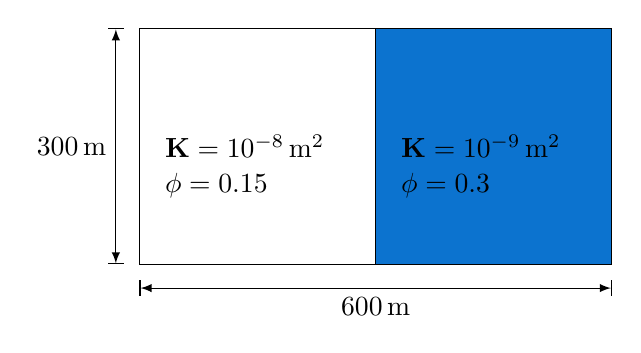
\begin{tikzpicture}[>=latex]
  % basic sketch
  \fill [dumuxBlue](3,0) rectangle ++(3,3);
  \draw (3,0) -- ++(0,3);
  \draw (0,0) rectangle ++(6,3);
  % arrows
  \draw [|<->|](0,-0.3) -- ++(6,0);
  \node at (3,-0.3)[anchor=north]{$\unit[600]{m}$};
  \draw [|<->|](-0.3,0) -- ++(0,3);
  \node at(-0.3,1.5)[anchor=east]{$\unit[300]{m}$};
  % labels
  \node [anchor=west] at (0.2,1.5){$\mathbf{K}=\unit[10^{-8}]{m^2}$};
  \node [anchor=west] at (0.2,1){$\phi=0.15$};
  \node [anchor=west] at (3.2,1.5){$\mathbf{K}=\unit[10^{-9}]{m^2}$};
  \node [anchor=west] at (3.2,1){$\phi=0.3$};
\end{tikzpicture}
\caption{Exercise 1d: Set-up of a model domain a heterogeneity. $\Delta x = \Delta y = \unit[20]{m}$.}
\label{tutorial-deoucpled:exercise1_d}
\end{figure}
When does the front cross the material border? In paraview, the option
\textit{View} $\rightarrow$ \textit{Animation View} is nice to get a rough
feeling of the time-step sizes.
\end{enumerate}

\subsubsection{Exercise 2}
For this exercise you should create a new problem file analogous to
the file \texttt{tutorialproblem\_decoupled.hh} (e.g. with the name
\texttt{ex2\_tutorialproblem\_decoupled.hh} and new spatial parameters
just like \texttt{tutorial\-spatialparams\_decoupled.hh}. These files need to
be included in the file \texttt{tutorial\_decoupled.cc}.

Each new files should contain the definition of a new class with a
name that relates to the file name, such as \texttt{Ex2TutorialProblemDecoupled}.
Make sure that you also adjust the guardian
macros in lines \ref{tutorial-decoupled:guardian1} and \ref{tutorial-decoupled:guardian2}
 in the header files (e.g. change \\
\texttt{DUMUX\_TUTORIALPROBLEM\_DECOUPLED\_HH} to
\texttt{DUMUX\_EX2\_TUTORIALPROBLEM\_DECOUPLED\_HH}).  Beside also adjusting the guardian macros,
the new problem file should define and use a new type tag for the problem as well as a new problem class
e.g. \texttt{Ex2TutorialProblemDecoupled}. Make sure to assign your newly defined spatial
parameter class to the \texttt{SpatialParams} property for the new
type tag.

After this, change the domain size (parameter input file) to match the domain described
by figure \ref{tutorial-decoupled:ex2_Domain}. Adapt the problem class
so that the boundary conditions are consistent with figure
\ref{tutorial-decoupled:ex2_BC}. Initially, the domain is fully saturated
with water and the pressure is $p_w = 2 \times 10^5 \, \text{Pa}$ . Oil
infiltrates from the left side. Create a grid with $20$ cells in
$x$-direction and $10$ cells in $y$-direction. The simulation time
should be set to $\unit[1e6]{s}$.

Now include your new problem file in the main file and replace the
\texttt{TutorialProblemDecoupled} type tag by the one you've created and
compile the program.


\begin{figure}[ht]
\centering
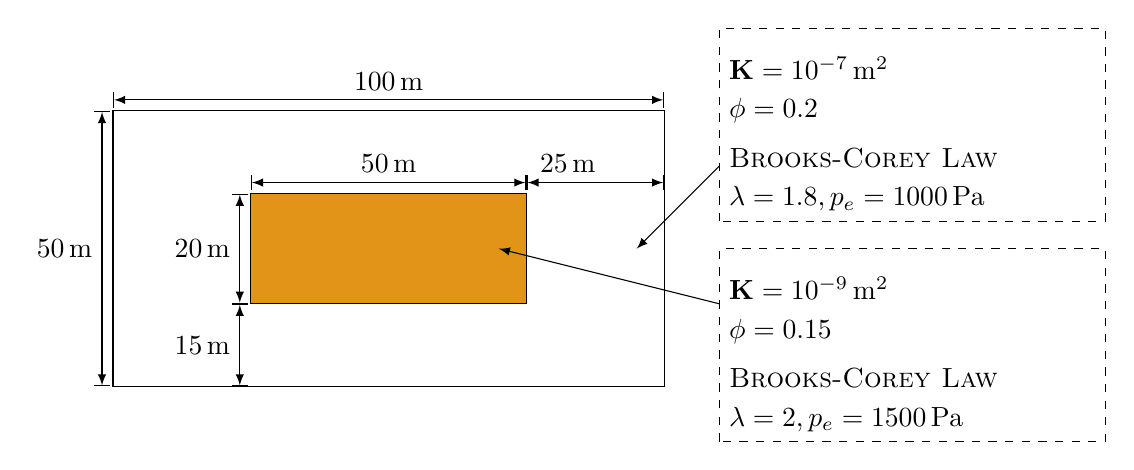
\begin{tikzpicture}[scale=0.7,>=latex]
  % basic sketch
  \draw (0,0) rectangle ++(10,5);
  \draw [fill=dumuxYellow] (2.5,1.5) rectangle ++(5,2);
  % arrows
  \draw[|<->|] (-0.2,0) -- ++(0,5);
  \node [anchor=east] at (-0.2,2.5){$\unit[50]{m}$};
  \draw[|<->|] (0,5.2) -- ++(10,0);
  \node [anchor=south] at (5,5.2){$\unit[100]{m}$};
  \draw[|<->|] (2.3,1.5) -- ++(0,2);
  \node [anchor=east] at (2.3,2.5){$\unit[20]{m}$};
  \draw[|<->|] (2.3,0) -- ++(0,1.5);
  \node [anchor=east] at (2.3,0.75){$\unit[15]{m}$};
  \draw[|<->|] (2.5,3.7) -- ++(5,0);
  \node [anchor=south] at (5,3.7){$\unit[50]{m}$};
  \draw[|<->|] (7.5,3.7) -- ++(2.5,0);
  \node [anchor=south] at (8.25,3.7){$\unit[25]{m}$};
  % labels
  \draw [dashed] (11,3) rectangle ++(7,3.5);
  \node [anchor=south west] at (11,5.4){$\mathbf{K} = \unit[10^{-7}]{m^2}$};
  \node [anchor=south west] at (11,4.6){$\phi = 0.2$};
  \node [anchor=south west] at (11,3.8){\textsc{Brooks-Corey Law}};
  \node [anchor=south west] at (11,3.0){$\lambda = 1.8, p_e = \unit[1000]{Pa}$};
  \draw [->] (11,4) -- (9.5,2.5);
  \draw [dashed] (11,-1) rectangle ++(7,3.5);
  \node [anchor=south west] at (11,1.4){$\mathbf{K} = \unit[10^{-9}]{m^2}$};
  \node [anchor=south west] at (11,0.6){$\phi = 0.15$};
  \node [anchor=south west] at (11,-0.2){\textsc{Brooks-Corey Law}};
  \node [anchor=south west] at (11,-1.0){$\lambda = 2, p_e = \unit[1500]{Pa}$};
  \draw [->] (11,1.5) -- (7,2.5);
\end{tikzpicture}
\caption{Set-up of the model domain and the soil parameters}\label{tutorial-decoupled:ex2_Domain}
\end{figure}

\begin{figure}[ht]
\centering
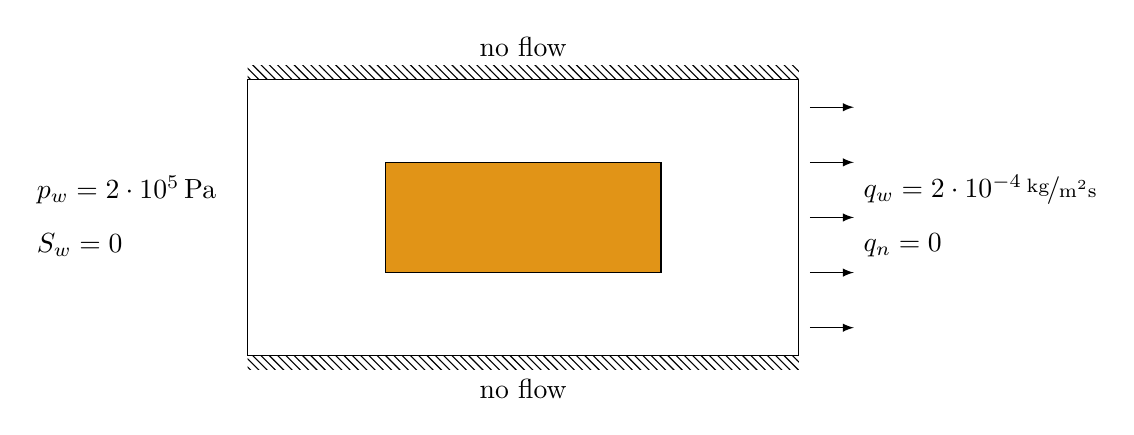
\begin{tikzpicture}[scale=0.7,>=latex]
  % basic sketch
  \fill [pattern=north west lines] (0,0) rectangle ++(10,-0.25);
  \fill [pattern=north west lines] (0,5) rectangle ++(10,0.25);
  \draw (0,0) rectangle ++(10,5);
  \draw [fill=dumuxYellow] (2.5,1.5) rectangle ++(5,2);
  \foreach \y in {0.5,1.5,...,4.5}
    \draw [->](10.2,\y) -- ++(0.8,0);
  % labels
  \node [anchor=south] at (5,5.25){no flow};
  \node [anchor=north] at (5,-0.25){no flow};
  \node [anchor=west] at(11,2){$q_n = 0$};
  \node [anchor=west] at(11,3){$q_w = \unitfrac[2 \cdot 10^{-4}]{kg}{m^2 s}$};
  \node [anchor=west] at(-4,2){$S_w = 0$};
  \node [anchor=west] at(-4,3){$p_w = \unit[2 \cdot 10^5]{Pa}$};
\end{tikzpicture}
\caption{Boundary Conditions}\label{tutorial-decoupled:ex2_BC}
\end{figure}

\begin{itemize}
 \item What happens if you increase the resolution of the grid? Hint: Paraview
 can visualize the time-steps via the ``Animation View'' (to be enabled unter the button \textit{View}).
 \item Set the CFL-factor to 1 and investigate the saturation: Is the value range reasonable?
 \item Further increase the CFL-factor to 2 and investigate the saturation.
\end{itemize}

\subsubsection{Exercise 3: Parameter file input}
As you have experienced, compilation takes quite some time. Therefore, \Dumux
provides a simple method to read in parameters (such as simulation end time or
modelling parameters) via \texttt{Paramter Input Files}. The tests in the Test-folder
\texttt{/test/} already use this system.\\
If you look at the Application in \texttt{/test/implicit/2p/}, you see that
the main file looks rather empty: The parameter file \texttt{test\_box2p.input}
is read by a standard start procedure, which is called in the main function.
This should be adapted for your problem at hand. The program run has to be
called with the parameter file as argument. As this is a basic \Dumux feature,
the procedure is the equivalent in the decoupled as in the box models.
In the code, parameters can be read via the macro
\texttt{GET\_RUNTIME\_PARAM(TypeTag, Scalar, MyWonderfulGroup.MyWonderfulParameter);}.
In \texttt{test\_2p}, \texttt{MyWonderfulGroup} is the group \texttt{SpatialParams}
- any type of groups is applicable, if the group definition in the parameter file
is enclosed in square brackets. The parameters are then listed thereafter.
Try and use as much parameters as possible via the input file, such as lens
dimension, grid resolution, soil properties etc. In addition, certain parameters
that are specific to the model, such as the \texttt{CFL}-factor, can be assigned
in the parameter file without any further action.

\subsubsection{Exercise 4}
Create a new file for benzene called \texttt{benzene.hh} and implement
a new fluid system. (You may get a hint by looking at existing fluid
systems in the directory \verb+/dumux/material/fluidsystems+.)

Use benzene as a new fluid and run the model of Exercise 2 with water
and benzene. Benzene has a density of $889.51 \, \text{kg} / \text{m}^3$
and a viscosity of $0.00112 \, \text{Pa} \, \text{s}$.

\subsubsection{Exercise 5: Time Dependent Boundary Conditions}
In this exercise we want to investigate the influence of time dependent boundary
conditions. For this, redo the steps of exercise 2 and create a new problem and
spatial parameters file.

After this, change the run-time parameters so that they match the
domain described by figure \ref{tutorial-decoupled:ex5_Domain}. Adapt
the problem class so that the boundary conditions are consistent with
figure \ref{tutorial-decoupled:ex5_BC}. Here you can see the time dependence of
the wetting saturation, where water infiltrates only during $10^5\,\text{s}$ and
$4 \cdot 10^5\,\text{s}$. To implement these time dependencies you need the actual
time $t_{n+1}=t_n + \Delta t$ and the endtime of the simulation. For this you can
use the methods \texttt{this->timeManager().time()}, \texttt{this->timeManager().timeStepSize()}
and \texttt{this->timeManager().endTime()}.

Initially, the domain is fully saturated with oil and the pressure is $p_w = 2 \times
10^5\,\text{Pa}$.  Water infiltrates from the left side. Create a grid
with $100$ cells in $x$-direction and $10$ cells in $y$-direction. The
simulation time should be set to $5 \cdot 10^5\,\text{s}$ with an
initial time-step size of $10\,\text{s}$. To avoid too big time-step sizes you
should set the parameter \texttt{MaxTimeStepSize} for the group \texttt{TimeManager}
(in your input file) to $\unit[100]{s}$. You should only create output files
every $100^{th}$ time-step (see exercise 1a). Then, you can compile the program.

\begin{figure}[ht]
\centering
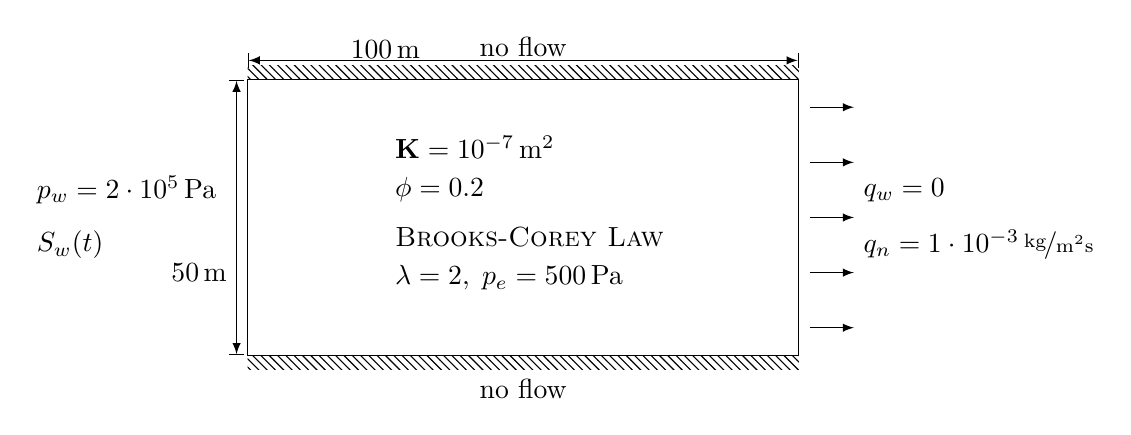
\begin{tikzpicture}[scale=0.7,>=latex]
  % basic sketch
  \fill [pattern=north west lines] (0,0) rectangle ++(10,-0.25);
  \fill [pattern=north west lines] (0,5) rectangle ++(10,0.25);
  \draw (0,0) rectangle ++(10,5);
  \foreach \y in {0.5,1.5,...,4.5}
    \draw [->](10.2,\y) -- ++(0.8,0);
  % arrows
  \draw[|<->|] (-0.2,0) -- ++(0,5);
  \node [anchor=east] at (-0.2,1.5){$\unit[50]{m}$};
  \draw[|<->|] (0,5.35) -- ++(10,0);
  \node [anchor=south] at (2.5,5.2){$\unit[100]{m}$};
  % labels
  \node [anchor=south] at (5,5.25){no flow};
  \node [anchor=north] at (5,-0.25){no flow};
  \node [anchor=west] at(11,2){$q_n = \unitfrac[1 \cdot 10^{-3}]{kg}{m^2 s}$};
  \node [anchor=west] at(11,3){$q_w = 0$};
  \node [anchor=west] at(-4,2){$S_w(t)$};
  \node [anchor=west] at(-4,3){$p_w = \unit[2 \cdot 10^5]{Pa}$};
  \node [anchor=south west] at (2.5,3.4){$\mathbf{K} = \unit[10^{-7}]{m^2}$};
  \node [anchor=south west] at (2.5,2.6){$\phi = 0.2$};
  \node [anchor=south west] at (2.5,1.8){\textsc{Brooks-Corey Law}};
  \node [anchor=south west] at (2.5,1.0){$\lambda = 2, \; p_e = \unit[500]{Pa}$};
\end{tikzpicture}
\caption{Set-up of the model domain and the soil parameters}\label{tutorial-decoupled:ex5_Domain}
\end{figure}

%  \draw (0,0) sin (5,5) cos (10,0);
\begin{figure}[ht]
\centering
\begin{tikzpicture}[scale=0.9,>=latex]
    % Draw axes
    \draw [<->,thick] (0,6) node (yaxis) [above] {$S_w$}
        |- (11,0) node (xaxis) [right] {time\,[s]};
    \draw plot[smooth,samples=100,domain=0:1] (6*\x + 2 ,{5*sin((\x)*pi r)});
	\draw [dashed] (0,5) -- (5,5);

    % axes labeling
    \draw [-] (-0.1,5) -- (0.1,5);
    \node [anchor=west] at(-0.5,5){$1$};
    \draw [-] (-0.1,0) -- (0.1,0);
    \node [anchor=west] at(-0.5,0){$0$};
    \draw [-] (2,0.1) -- (2,-0.1);
    \node [anchor=west] at(1.5,-0.4){$1\cdot10^{5}$};
    \draw [-] (8,0.1) -- (8,-0.1);
    \node [anchor=west] at(7.5,-0.4){$4\cdot10^{5}$};
    \draw [-] (10,0.1) -- (10,-0.1);
    \node [anchor=west] at(9.5,-0.4){$5\cdot10^{5}$};

    \node [anchor=base] at (5,2){$\sin(\pi\frac{\text{time}-10^5}{3\cdot 10^5 })$};
\end{tikzpicture}
\caption{Time Dependent Boundary Conditions}\label{tutorial-decoupled:ex5_BC}
\end{figure}

\begin{itemize}
 \item Open paraview and plot the values of $S_w$ at time $\unit[5 \cdot 10^5]{s}$
 over the $x-$axis.\\ (\texttt{Filter->Data Analysis->Plot Over Line})
 \item What happens without any time-step restriction?
\end{itemize}

\subsubsection{Exercise 6}
If both the coupled and the decoupled tutorial are completed, one should have
noticed that the function arguments in the problem function differ slighty, as
the numerical models differ. However, both are functions that depend on space,
so both models can also work with functions based ond \mbox{\texttt{...AtPos(GlobalPosition \& globalPos)}},
no matter if we model coupled or decoupled. Try to formulate a spatial parameters
file that works with both problems, the coupled and the decoupled. Therein, only
use functions at the position.


\section{Further Practice}
\label{tutorial-furtherpractice}

If there is a need for further practice, we refer here to the test problems that
are already implemented in \Dumux. Several examples for all models
can be found in the \texttt{test}-directory. An overview over the available test
cases can be found in the class documentation \url{http://www.dumux.org/documentation.php}.
There you also find a \emph{feature-list} for the individual tests.%TODO

Another possibility to gain more experience with \Dumux is the \texttt{dumux-lecture} module
that contains different application examples that are used in the lectures at the 
Department of Hydromechanics and Modelling of Hydrosystems in Stuttgart.
The \texttt{dumux-lecture} module can be obtained as follows:
\begin{lstlisting}[style=Bash]
$ git clone https://git.iws.uni-stuttgart.de/dumux-repositories/dumux-lecture.git
\end{lstlisting}
The module is structured based on the different lectures: 
\begin{itemize}
\item mm: Multiphase Modelling,
\item efm: Environmental Fluid Mechanics,
\item mhs: Modelling of Hydrosystems.
\end{itemize}
The majority of applications is covered in the course Multiphase Modelling (mm), 
while there are also some basic examples from the
courses Environmental Fluid Mechanics (efm) and Modelling of Hydrosystems (mhs). 
These applications are primarily designed to enhance the understanding of conceptualizing the
governing physical processes and their implementation in a numerical simulator. 
Different aspects of modelling multi-phase multi-component flow and transport processes are shown.
The lectures focus on questions like, e. g., the assignment of boundary conditions, the choice of the 
appropriate physics for a given problem (which phases, which components), discretization issues,
time stepping. You can find, e. g., a comparison of different two-phase flow problems: The
more simple approach considers two immiscible fluids while components in both phases with interphase
mass transfer are considered in the more complex approach.
All scenarios and their physical background are explained in additional .tex-files,
which are provided in sub-directories named \texttt{description}. The following test cases are 
contained in the \texttt{dumux-lecture} module:
\begin{itemize}
\item \texttt{buckleyleverett}: The Buckley-Leverett Problem is a classical porous media flow show case
\item \texttt{co2plume}: Analysis of the influence of the gravitational number on the $\text{CO}_2$ plume 
\item \texttt{columnxylene}: A VEGAS experiment
\item \texttt{convectivemixing}: A test case related to CO$_2$ storage
\item \texttt{fuelcell}%TODO
\item \texttt{heatpipe}: A show case for two-phase two-component flow with heat fluxes
\item \texttt{heavyoil}: Steam assisted gravity drainage (SAGD)
\item \texttt{henryproblem}: A show case related to salt water intrusion
\item \texttt{mcwhorter}: The McWhorter Problem is a classical porous media flow show case
\item \texttt{naplinfiltration}: Infiltration of non-aqueous phase liquid (NAPL) into soil
\item \texttt{remediationscenarios}: Test case for NAPL contaminated unsaturated soils
\item \texttt{groundwater}: Simple groundwater flow case for the course Modelling of Hydrosystems (mhs)
\item Different single/two-phase, single/two-component problems: Examples from the course Environmental Fluid Mechanics (efm)
\end{itemize}


\chapter{Overview and Infrastructure}
This chapter provides an overview of the general structure in \Dumux \ref{sc_structure}
and gives help for basic work with \Dumux
(\ref{sc_newfoldersetup},\ref{sc_parameterfiles},\ref{sc_restartsimulations},\ref{sc_guidelines},\ref{sc_developingdumux}).
Further it present useful external tools \ref{sc_externaltools} and basic
concepts \ref{sc_linearsystem}.
\section{Directory Structure}
\todo[inline]{Wollen wir hier alle Unterordner kurz vorstellen und \emph{kurz} erklären,
  was in deren Unterordnern zu finden ist?}
We briefly describe the directory structure of \Dumux in terms
of subdirectories, source files, and tests. For more details,
the Doxygen documentation should be considered.
\Dumux comes in form of a DUNE module \texttt{dumux}.
It has a similar structure as other DUNE modules like \texttt{dune-grid}.
The following subdirectories are within the module's root directory,
from now on assumed to be \texttt{/}:
\begin{itemize}
\item \texttt{bin}: contains binaries, e.g. used for the automatic testing
\item \texttt{CMake}: the configuration options
for building \Dumux using CMake. See the file \texttt{INSTALL.cmake} in
the root directory of \texttt{dumux} for details. Of course,
it is also possible to use the DUNE buildsystem just like for the other
DUNE modules.
\item \texttt{doc}: contains the Doxygen documentation in \texttt{doxygen},
this handbook in \texttt{handbook}, and the \Dumux logo in various formats in
\texttt{logo}. The html documentation produced by Doxygen can be accessed as usual,
namely, by opening \texttt{doc/doxygen/html/index.html} with a web browser.
\item \texttt{dumux}: the \Dumux source files. See Section \ref{sec:dumux} for details.
\item \texttt{test}: tests for each numerical model and the property system.
See Section \ref{sec:test} for details.
\item \texttt{tutorial}: contains the tutorials described in Chapter \ref{chp:tutorial}.
\end{itemize}


\subsection{The directory \texttt{dumux}}
\label{sec:dumux}

The directory \texttt{dumux} contains the \Dumux source files. It consists of the
following subdirectories (see Figure \ref{fig:dumux-structure}):

\begin{itemize}

\item \texttt{implicit}:
the general fully implicit method is contained in the subdirectory \texttt{common}.
The subdirectories \texttt{box} and \texttt{cellcentered} contain the code for the according
discretization types. They also contain files \texttt{..fvelementgeometry.hh} employed
by the box or cc method to extract the dual mesh geometry information out of the primal one.
Each of the other subdirectories contain a derived specific numerical model.
% The files \texttt{pdelabboxassembler.hh} and \texttt{pdelabboxlocaloperator.hh} allow the use of the DUNE module \texttt{dune-pdelab}.

\item \texttt{common}:
general stuff like the property system and the time management for the
fully coupled as well as the decoupled models,
% the interface for the Pardiso direct solver library \cite{Pardiso},
and the \texttt{start.hh} file that includes the common routine for starting a model called in the main function.

\item \texttt{decoupled}:
 numerical models to solve the pressure equation as part of the fractional flow
 formulation. The specific models are contained
 in corresponding subdirectories. In each model folder are subdirectories for the
 implicit pressure equation sorted by the employed discretization method, and for the
 explicit transport equation. The general decoupled formulation for the implicit
 pressure explicit transport formulation can be found in the subdirectory \texttt{common}.

% \item \texttt{fractionalflow}:
% the (non-compositional) fractional flow model, which utilizes the IMPES method
% contained in the subdirectory \texttt{impes}.

% \item \texttt{functions}:
% the Crouzeix--Raviart function implemented in the style of \texttt{dune-disc}'s P1 function.

% \item \texttt{fvgeometry}:
% employed by the box method to extract the dual mesh geometry information out of the
% primal one.

\item \texttt{io}: additional in-/output possibilities like restart files, gnuplot-interface
and a VTKWriter extension.

\item \texttt{material}: everything related to material parameters and
constitutive equations. The properties of a pure chemical substance (e.g. water) or
pseudo substance (e.g. air) can be found in the subdirectory \texttt{components}
with the base class \texttt{components/component.hh}. The fluidsytem in the folder
\texttt{fluidsystems} collects the information from the respective component and
binary coefficients files, and contains the fluid characteristics of phases
(e.g. viscosity, density, enthalpy, diffusion coefficients) for compositional or non-compositional multi-phase flow.

The base class for all spatially dependend variables -- like permeability and porosity  --
can be found in \texttt{spatialparams}. The base class in \texttt{implicitspatialparameters.hh}
also provides spatial averaging routines. All other spatial properties are specified in the specific
 files of the respective models. Furthermore, the constitutive relations --
 e.g. $p_c(S_w) $ -- are in \texttt{fluidmatrixinteractions},
while the necessary binary coefficients like the Henry coefficient or binary diffusion coefficients are definded in
 \texttt{binarycoefficients}.


\item \texttt{nonlinear}: Newton's method.


% \item \texttt{operators}: based on \texttt{dune-disc}, assembly operators for Crouzeix--Raviart
% elements and mimetic finite differences.
%
%
% \item \texttt{pardiso}: interface to the Pardiso direct solver library, \cite{Pardiso}.
%
%
% \item \texttt{shapefunctions}:  Crouzeix--Raviart element shape functions.
%
%
% \item \texttt{timedisc}: time discretization for the decoupled models.
%
%
% \item \texttt{transport}: numerical models to solve the pressure equation
% as part of the fractional flow formulation analogous to the \texttt{diffusion}
% directory. Moreover, the compositional decoupled models are included here.


\end{itemize}



\subsection{The directory \texttt{test}}
\label{sec:test}
The directory \texttt{test} contains a test for each numerical model and for
the property system. The tests for the property system can be found in \texttt{common}.
The subfolder \texttt{implicit} contains tests for the fully
coupled models (\texttt{1p},  \texttt{1p2c},  \texttt{2p},  \texttt{2p2c},
\texttt{2p2cni},  \texttt{2pni}, \texttt{3p3c},  \texttt{3p3cni},  \texttt{mpnc}
and \texttt{richards}), while the subdirectory \texttt{decoupled} corresponds to the decoupled models.
Each subdirectory contains one or more program files \texttt{test\_*.cc}, where \texttt{*} usually is the
name of the folder. Moreover, the problem definitions can be found
in the \texttt{*problem.hh} files and the definition of the spatially dependent
parameters in \texttt{*spatialparameters.hh}. Simply executing the tests should either run the
full test or give a list of required command line arguments. After test execution,
VTK output files should have been generated.
For more detailed descriptions of the tests, the problem definitions and their corresponding
Doxygen documentation should be considered.

\begin{sidewaysfigure}
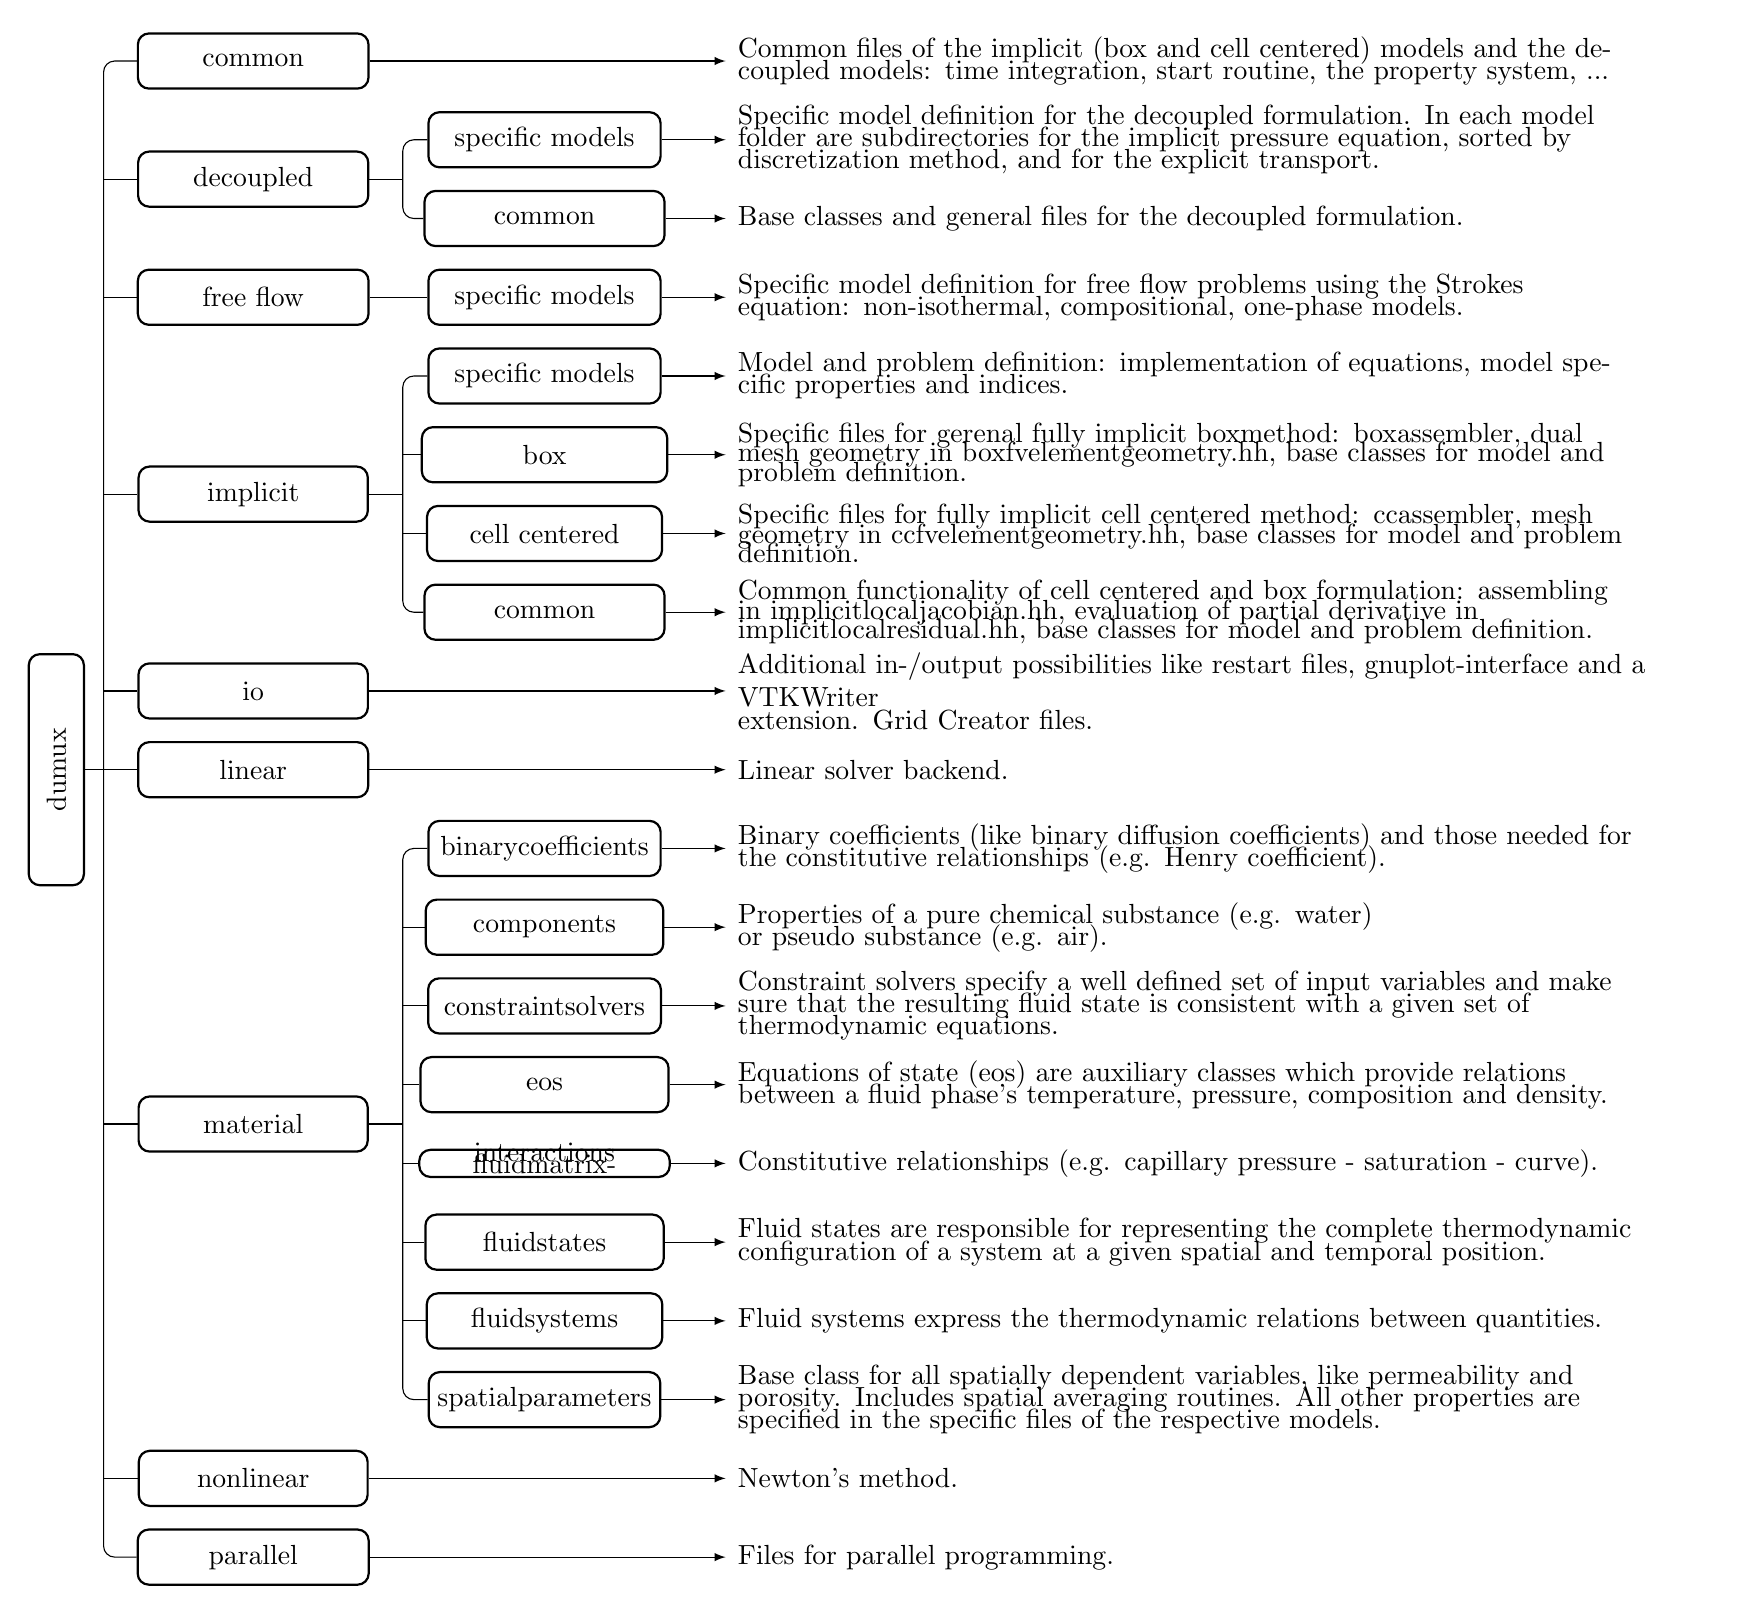
\begin{tikzpicture}[>=latex,inner xsep=0.15cm,rounded corners]
\node [minimum height=0.7cm,draw,inner xsep=0.94cm,rotate=90,thick] (d) at(-2,0) {dumux};
\node [minimum height=0.7cm,draw,inner xsep=1.03cm,thick] (lin) at(0.5,0) {linear};
\node [minimum height=0.7cm,draw,inner xsep=1.32cm,thick] (io) at(0.5,1) {io};

\node [minimum height=0.7cm,draw,inner xsep=0.87cm,thick] (imp) at(0.5,3.5) {implicit};
 \node [minimum height=0.7cm,draw,inner xsep=0.88cm,thick] (c1) at(4.2,2) {common};
 \node [minimum height=0.7cm,draw,inner xsep=0.54cm,thick] (cell) at(4.2,3) {cell centered};
 \node [minimum height=0.7cm,draw,inner xsep=1.28cm,thick] (box) at(4.2,4) {box};
 \node [minimum height=0.7cm,draw,inner xsep=0.33cm,thick] (spec1) at(4.2,5) {specific models};

\node [minimum height=0.7cm,draw,inner xsep=0.82cm,thick] (free) at(0.5,6) {free flow};
  \node [minimum height=0.7cm,draw,inner xsep=0.33cm,thick] (spec2) at(4.2,6) {specific models};

\node [minimum height=0.7cm,draw,inner xsep=0.7cm,thick] (dec) at(0.5,7.5) {decoupled};
 \node [minimum height=0.7cm,draw,inner xsep=0.88cm,thick] (c2) at(4.2,7) {common};
 \node [minimum height=0.7cm,draw,inner xsep=0.33cm,thick] (spec3) at(4.2,8) {specific models};

\node [minimum height=0.7cm,draw,inner xsep=0.82cm,thick] (c3) at(0.5,9) {common};

\node [minimum height=0.7cm,draw,inner xsep=0.82cm,thick] (m) at(0.5,-4.5) {material};
 \node [minimum height=0.7cm,draw,thick] (bin) at(4.2,-1) {binarycoefficients};
 \node [minimum height=0.7cm,draw,inner xsep=0.6cm,thick] (comp) at(4.2,-2) {components};
 \node [minimum height=0.7cm,draw,inner xsep=0.2cm,thick] (con) at(4.2,-3) {constraintsolvers};
 \node [minimum height=0.7cm,draw,inner xsep=1.34cm,thick] (eos) at(4.2,-4) {eos};
 \node [inner ysep=0.05cm,draw,text width=2cm,align=center,inner xsep=0.59cm,thick] (fi) at(4.2,-5) {fluidmatrix-\\[-16pt]interactions};
 \node [minimum height=0.7cm,draw,inner xsep=0.73cm,thick] (fstate) at(4.2,-6) {fluidstates};
 \node [minimum height=0.7cm,draw,inner xsep=0.56cm,thick] (fsys) at(4.2,-7) {fluidsystems};
 \node [minimum height=0.7cm,draw,inner xsep=0.11cm,thick] (s) at(4.2,-8) {spatialparameters};

\node [minimum height=0.7cm,draw,inner xsep=0.74cm,thick] (non) at(0.5,-9) {nonlinear};
\node [minimum height=0.7cm,draw,inner xsep=0.9cm,thick] (para) at(0.5,-10) {parallel};

\draw (d)--(lin);
\draw (-1.4,0)--(-1.4,9)--(c3);
\draw (-1.4,0)--(-1.4,-10)--(para);
\draw (-1.4,7.5)--(dec);
\draw (-1.4,6)--(free);
\draw (-1.4,3.5)--(imp);
\draw (-1.4,1)--(io);
\draw (-1.4,-4.5)--(m);
\draw (-1.4,-9)--(non);

\draw (dec)--(2.4,7.5);
\draw (spec3)--(2.4,8)--(2.4,7)--(c2);
\draw (free)--(spec2);
\draw (imp)--(2.4,3.5);
\draw (spec1)--(2.4,5)--(2.4,2)--(c1);
\draw (box)--(2.4,4);
\draw (cell)--(2.4,3);
\draw (m)--(2.4,-4.5);
\draw (bin)--(2.4,-1)--(2.4,-8)--(s);
\draw (comp)--(2.4,-2);
\draw (con)--(2.4,-3);
\draw (eos)--(2.4,-4);
\draw (fi)--(2.4,-5);
\draw (fstate)--(2.4,-6);
\draw (fsys)--(2.4,-7);

\draw [->](c3)--(6.5,9) node [right,text width=12.5cm,align=left]
  {Common files of the implicit (box and cell centered) models and the de-\\[-4pt]
   coupled models: time integration, start routine, the  property system, ...};
\draw [->](spec3)--(6.5,8) node [right,text width=12.5cm,align=left]
  {Specific model definition for the decoupled formulation. In each model \\[-4pt]
   folder are subdirectories for the implicit pressure  equation, sorted by \\[-4pt]discretization method, and for the explicit transport.};
\draw [->](c2)--(6.5,7) node [right,text width=12.5cm,align=left]
  {Base classes and general files for the decoupled formulation.};
\draw [->](spec2)--(6.5,6) node [right,text width=12.5cm,align=left]
  {Specific model definition for free flow problems using the Strokes \\[-4pt]
   equation: non-isothermal, compositional, one-phase models.};
\draw [->](spec1)--(6.5,5) node [right,text width=12.5cm,align=left]
  {Model and problem definition: implementation of equations, model spe-\\[-4pt]
   cific properties and indices.};
\draw [->](box)--(6.5,4) node [right,text width=12.5cm,align=left]
  {Specific files for gerenal fully implicit boxmethod: boxassembler, dual \\[-5pt]
   mesh geometry in boxfvelementgeometry.hh, base classes for model and \\[-5pt]problem definition.};
\draw [->](cell)--(6.5,3) node [right,text width=12.5cm,align=left]
  {Specific files for fully implicit cell centered method: ccassembler, mesh \\[-5pt]
   geometry in ccfvelementgeometry.hh, base classes for model and problem \\[-5pt]definition.};
\draw [->](c1)--(6.5,2) node [right,text width=12.5cm,align=left]
  {Common functionality of cell centered and box formulation: assembling \\[-5pt]
   in implicitlocaljacobian.hh, evaluation of partial derivative in \\[-5pt]implicitlocalresidual.hh, base classes for model and problem definition.};
\draw [->](io)--(6.5,1) node [right,text width=12.5cm,align=left]
  {Additional in-/output possibilities like restart files, gnuplot-interface and a VTKWriter \\[-4pt]
   extension. Grid Creator files.};
\draw [->](lin)--(6.5,0) node [right,text width=12.5cm,align=left] {Linear solver backend.};
\draw [->](bin)--(6.5,-1) node [right,text width=12.5cm,align=left]
  {Binary coefficients (like binary diffusion coefficients) and those needed for \\[-4pt]
   the constitutive relationships (e.g. Henry coefficient).};
\draw [->](comp)--(6.5,-2) node [right,text width=12.5cm,align=left]
  {Properties of a pure chemical substance (e.g. water) \\[-4pt]or pseudo substance (e.g. air).};
\draw [->](con)--(6.5,-3) node [right,text width=12.5cm,align=left]
  {Constraint solvers specify a well defined set of input variables and make \\[-4pt]
   sure that the resulting fluid state is consistent with a given set of \\[-4pt]thermodynamic equations.};
\draw [->](eos)--(6.5,-4) node [right,text width=12.5cm,align=left]
  {Equations of state (eos) are auxiliary classes which provide relations \\[-4pt]
   between a fluid phase's temperature, pressure, composition and density.};
\draw [->](fi)--(6.5,-5) node [right,text width=12.5cm,align=left]
  {Constitutive relationships (e.g. capillary pressure - saturation - curve).};
\draw [->](fstate)--(6.5,-6) node [right,text width=12.5cm,align=left]
  {Fluid states are responsible for representing the complete thermodynamic \\[-4pt]
   configuration of a system at a given spatial and temporal position.};
\draw [->](fsys)--(6.5,-7) node [right,text width=12.5cm,align=left]
  {Fluid systems express the thermodynamic relations between quantities.};
\draw [->](s)--(6.5,-8) node [right,text width=12.5cm,align=left]
  {Base class for all spatially dependent variables, like permeability and \\[-4pt]
   porosity. Includes spatial averaging routines. All other properties are \\[-4pt]
   specified in the specific files of the respective models.};
\draw [->](non)--(6.5,-9) node [right,text width=12.5cm,align=left]
  {Newton's method.};
\draw [->](para)--(6.5,-10) node [right,text width=12.5cm,align=left]
  {Files for parallel programming.};
\end{tikzpicture}
\caption{Structure of the directory \texttt{dumux} containing the \Dumux source files.
\todo[inline]{bei dieser Skizze sollten wir auch schauen ob die noch aktuell ist.}}
\label{fig:dumux-structure}
\end{sidewaysfigure}

\section{Setup of a New Folder and New Tests}

\paragraph{Setting up a New Folder}
In this section it is described how to set up a new folder and how to tell
the build system, that there is a new one.

\begin{enumerate}[1)]
 \item create new folder with content
 \item adapt the \verb+CMakeList.txt+ in the folder above and add a line with
       \verb+add_subdirectory(NEW\_FOLDER)+
 \item adapt the \verb+CMakeList.txt+ in the newly created folder and add your test
       (see below for more information)
 \item go to your \texttt{build}-directory and type \verb+make+ to
       reconfigure the system
\end{enumerate}

\paragraph{Adding a New Test Program}
\noindent To simply add a new executable use the following macro. The test will \emph{not} be built
automatically when running \texttt{ctest}. You have to compile it manually by
\texttt{make test\_program}.
\begin{verbatim}
add_executable_all(test\_program test\_program.cc)
\end{verbatim}

\noindent To add a test, which should be compiled when running \texttt{ctest}, use the
\texttt{add\_dumux\_test} macro. You can decide whether, the program should be run
after compiling or not.
Please note that the name of the test (first argument) must be unique, whereas the name
of the executable (second argument) can occur multiple times.
\begin{verbatim}
add_dumux_test(test\_program test\_program test\_program.cc
  test\_program # add this line, if the program should also be run
  )
\end{verbatim}

\noindent To add a test which should be run and compared to a reference solution when using
\texttt{ctest}, please use the following structure. The macro \texttt{\${CMAKE\_SOURCE\_DIR}}
gives the location of your source code. The macro \texttt{\${CMAKE\_CURRENT\_BINARY\_DIR}}
gives the current folder with the executable.
\begin{verbatim}
add_dumux_test(test\_program test\_program test\_program.cc
  ${CMAKE_SOURCE_DIR}/bin/runTest.sh
  ${CMAKE_SOURCE_DIR}/bin/fuzzycomparevtu.py
  LOCATION_TO_THE_REFERNCE_SOLUTION/test\_program-reference.vtu
  ${CMAKE_CURRENT_BINARY_DIR}/test\_program-00009.vtu
  ${CMAKE_CURRENT_BINARY_DIR}/test\_program)
\end{verbatim}

\paragraph{Committing a New older to SVN}
For those who work with Subversion (\texttt{svn}) and want to commit a newly setup folder to the repository some basics are
given in this paragraph. For further reading please check out the Subversion User Manual found at \cite{APACHE-SUBVERSION-HP}
where you will also find a "High Speed Turorial" in the appendix. \\
The four most important commands are \texttt{svn checkout}, \texttt{svn update},  \texttt{svn add}
and \texttt{svn commit}. The first one (\texttt{svn checkout}) you probably already know from the \Dumux installation.
It will create a copy of the trunk version from the svn server on your local system. Use \texttt{svn update} to get the
latest changes in the repository (commits from other users). In order to add a new folder to the repository the following
steps have to be taken:

\begin{enumerate}[1)]
\item \texttt{svn update}: The first step is to update your \Dumux. You should execute this command in your
      dumux-stable or dumux-devel folder.
\item \texttt{svn add --depth=empty YOURFOLDER}: This command adds the folder without its content.
\item In your folder: use \texttt{svn add YOURFILES} to add your files. Generally, you should only add
      your header files (.hh), your source files (.cc), your input file (.input), if required your
      grid file (.dgf) or if necessary other text-based files. Please do not upload (large) binary files.
\item Type \texttt{svn status} in your \texttt{dumux}-root directory the see all the file changes.
      \texttt{?} indicates possible forgotten files. Make sure that you include all necessary
      files in your commit.
\item Use \texttt{svn commit} from the directory level containing your folder. This uploads all your changes to the
      svn server. You will be asked to briefly explain the content of your commit in an editor.
\end{enumerate}

\section{Parameters in \Dumux}
\label{sc_parameterfiles}
Simulation parameters can be parsed to the program via a parameter file or the command line.
A list of all available parameters is provided in the Doxygen documentation
of the file \texttt{parameterfile}, which is accessible via \texttt{Modules -> Parameters}.

After having run the example application from section \ref{quick-start-guide} you will
get the following output at the end of the simulation run
\footnote{If you did not get the output, restart the application the following way:
\texttt{./test{\_}box2p -PrintParameters true},
this will print the parameters once your simulation is finished}:
\begin{lstlisting}[style=Bash]
# Run-time specified parameters:
[ Grid ]
File = "./grids/test_2p.dgf"
[ Implicit ]
EnableJacobianRecycling = "1"
EnablePartialReassemble = "1"
[ Problem ]
Name = "lensbox"
[ SpatialParams ]
LensLowerLeftX = "1.0"
LensLowerLeftY = "2.0"
LensUpperRightX = "4.0"
LensUpperRightY = "3.0"
[ TimeManager ]
DtInitial = "250"
TEnd = "3000"
# DEPRECATED run-time specified parameters:
PrintParameters = "1"
# Replace by:
[ TimeManager ]
PrintParameters = "1"
# Compile-time specified parameters:
[ Implicit ]
EnableHints = "0"
MassUpwindWeight = "1"
MaxTimeStepDivisions = "10"
MobilityUpwindWeight = "1"
NumericDifferenceMethod = "1"
UseTwoPointFlux = "0"
[ LinearSolver ]
MaxIterations = "250"
PreconditionerRelaxation = "1"
ResidualReduction = "1e-06"
Verbosity = "0"
[ Newton ]
WriteConvergence = "0"
[ Problem ]
EnableGravity = "1"
[ TimeManager ]
MaxTimeStepSize = "1.79769e+308"
[ Vtk ]
AddVelocity = "0"
# UNUSED parameters:
ImportantVariable = "1"
\end{lstlisting}

A number of things can be learned:
\begin{itemize}
  \item \emph{run-time} parameters can be changed without re-compiling
  \item \emph{deprecated run-time} parameters will be removed in the next release
  \item \emph{compile-time} parameters cannot be overwritten by the input file
  \item \emph{unused} are not used by the simulation (maybe typo or wrong group)
\end{itemize}

All applications have a help message which you can read by giving
\texttt{--help} as a command line argument to the application.

For further details, please have a look for \texttt{Dune::ParameterTree}
in the \Dune documentation.

\section{Restart \Dumux Simulations}
\label{sc_restartsimulations}

\Dumux has some experimental support for check-pointing (restarting paused/stopped/crashed simulations).
You can restart a \Dumux simulation from any time point where a VTK file was written out.
This is currently only supported for sequential, non-adaptive simulations. For adaptive simulation
the full hierarchical grid has to be stored. This is usually done with the grid's \texttt{BackupRestoreFacility}.
There is currently no special support by \Dumux for that, but it is possible to implement
a restart using \texttt{BackupRestoreFacility} with plain Dune.

For VTK files the output can be read with the free function \texttt{loadSolution}. Grids can be read with
the \texttt{Dumux::VTKReader} or you can simply recreate the grid as you did in the first simulation run.

Unfortunately, writing double-precision floating point numbers to VTK files is only available with Dune master (will be in 2.7).
That's why we currently only support single precision restart, meaning some information will be lost if you are computing
in double precision.

The restart capabilities will hopefully be improved in future versions of \Dumux 3.
We are happy about any contributions (especially HDF5 / XDMF support, improvement of VTK support).

\section{Coding Guidelines}
\label{sc_guidelines}
Writing code in a readable manner is very important, especially
for future code developers (e.g. for adding features, debugging, etc.).
For the style guide and instructions how to contribute to \Dumux visit
\url{https://git.iws.uni-stuttgart.de/dumux-repositories/dumux/blob/master/CONTRIBUTING.md}.

\section{Developing \Dumux}
\label{sc_developingdumux}

\subsection{Communicate with \Dumux Developers}

\paragraph{Issues and Bug Tracking}
The bug-tracking system \emph{GitLab Issues} offers the possibility to report bugs or discuss new development requests.
Feel free to register (if you don't have a \emph{Git} account already) and to constribute
at \url{https://git.iws.uni-stuttgart.de/dumux-repositories/dumux/issues}.

\paragraph{Commits, Merges, etc.}
To be up-to-date with the latest changes made to any git-repository you can use RSS Feeds.
Simply click on \emph{Issues} or \emph{Activity} and then select a tab you are interested in
and use your favorite RSS-application for receiving the news.

\paragraph{Automatic Testing Dashboard}
The automatic testing using \emph{BuildBot} helps to constantly check the
\Dumux problems for compiling and running correctly. It is available at
\url{https://git.iws.uni-stuttgart.de/buildbot/#/builders}.

\paragraph{The General Mailing List:}
If you have questions, specific problems (which you really struggle to solve on your own),
or hints for the \Dumux-developers, please contact the mailing list \url{dumux@iws.uni-stuttgart.de}.
You can subscribe to the mailing list via
\url{https://listserv.uni-stuttgart.de/mailman/listinfo/dumux}, then you
will be informed about upcoming releases or events.

\subsection{Coding Guidelines}
Writing code in a readable manner is very important, especially
for future code developers (e.g. for adding features, debugging, etc.).
For the style guide and instructions how to contribute to \Dumux visit
\url{https://git.iws.uni-stuttgart.de/dumux-repositories/dumux/blob/master/CONTRIBUTING.md}.


\subsection{Tips and Tricks}
\Dumux users and developers at the LH2 are also referred to the internal Wiki for
more information.

\paragraph{Optimized computation vs debugging}
\Dune and \Dumux are built with the help of \texttt{dunecontrol}, as explained on page \pageref{buildIt}.
Per default, \Dumux is compiled using optimization options, which leads to faster runtimes but is unsuitable
for debugging. For debug opts you can set \texttt{DCMAKE_BUILD_TYPE} to \texttt{Debug} or \texttt{RelWithDebInfo}
in your options file. You can also do this in any of the \texttt{CMakeLists.txt} in Dumux by adding:

\begin{lstlisting}[style=Shell]
set(CMAKE_BUILD_TYPE Debug)
\end{lstlisting}

Afterwards rerun cmake again (run cmake <path-to-build-dir>).

\paragraph{Dunecontrol for selected modules}
A complete build using \texttt{dunecontrol} takes some time. In many cases not all modules need to be re-built.
Pass the flag \texttt{--only=dumux} to \texttt{dunecontrol} for configuring or building only \Dumux. A more
complex example would be the use of an additional module. Then you have to configure and build only \Dune{}-grid
and \Dumux by adding \texttt{--only=MODULE,dumux}.

\paragraph{Patching Files or Modules}
If you want to send changes to an other developer of \Dumux providing patches
can be quite smart. To create a patch simply type:
\begin{lstlisting}[style=Bash]
$ git diff > PATCHFILE
\end{lstlisting}
\noindent which creates a text file containing all your changes to the files
in the current folder or its subdirectories.
To apply a patch in the same directory type:
\begin{lstlisting}[style=Bash]
$ patch -p1 < PATCHFILE
\end{lstlisting}

%TODO: currently, no DUNE patches necessary! Thus, this section is commented and the missing refrence would be bad.
% Uncomment the following statement again when patches might be necessary.
% See \ref{sc:patchingDUNE} if you need to apply patches to \Dumux or \Dune.

\paragraph{File Name and Line Number by Predefined Macro}
If you want to  know where some output or debug information came from, use the predefined
macros \texttt{\_\_FILE\_\_} and \texttt{\_\_LINE\_\_}:
\begin{lstlisting}[style=DumuxCode]
std::cout << "# This was written from "<< __FILE__ << ", line " << __LINE__ << std::endl;
\end{lstlisting}

\paragraph{Using \Dune Debug Streams}
\Dune provides a helpful feature, for keeping your debug-output organized.
It uses simple streams like \texttt{std::cout}, but they can be switched on and off
for the whole project. You can chose five different levels of severity:
\begin{verbatim}
5 - grave (dgrave)
4 - warning (dwarn)
3 - info (dinfo)
2 - verbose (dverb)
1 - very verbose (dvverb)
\end{verbatim}
\noindent They are used as follows:
\begin{lstlisting}[style=DumuxCode]
// define the minimal debug level somewhere in your code
#define DUNE_MINIMAL_DEBUG_LEVEL 4
Dune::dgrave << "message"; // will be printed
Dune::dwarn << "message"; // will be printed
Dune::dinfo << "message"; // will NOT be printed
\end{lstlisting}

\paragraph{Make headercheck:}
To check one header file for all necessary includes to compile the contained code, use \texttt{make headercheck}.
Include the option \texttt{-DENABLE\_HEADERCHECK=1} in your opts file and run \texttt{dunecontrol}.
Then go to the top level in your build-directory and type \texttt{make headercheck} to check all headers
or press 'tab' to use the auto-completion to search for a specific header.

\section{External Tools}
\label{sc_externaltools}

\subsection{Eclipse}
There is an Eclipse style file which can be used for \Dumux.
\begin{enumerate}
  \item open in eclipse: \texttt{Window} $\rightarrow$ \texttt{Preferences} $\rightarrow$
        \texttt{C/C++}  $\rightarrow$ \texttt{Code Style} $\rightarrow$ \texttt{Formatter}
  \item press the \texttt{Import} button
  \item choose the file \texttt{eclipse\_profile.xml} from your dumux-devel directory
  \item make sure that now \Dumux is chosen in \texttt{Select a profile}
\end{enumerate}


\subsection{Git}
Git is a version control tool which we use.
The basic Git commands are:
\begin{itemize}
  \item \texttt{git checkout} receive a specified branch from the repository
  \item \texttt{git clone} clone a repository; creates a local copy
  \item \texttt{git diff} to see the actual changes compared to your last commit
  \item \texttt{git pull} pull changes from the repository; synchronizes the
  repository with your local copy
  \item \texttt{git push} push comitted changes to the repository;  synchronizes
  your local copy with the repository
  \item \texttt{git status} to check which files/folders have been changed
  \item \texttt{git gui} graphical user interface, helps selecting changes for
  a commit
\end{itemize}


\subsection{Gnuplot}
\label{gnuplot}
A gnuplot interface is available to plot or visualize results during a simulation run.
This is achieved with the help of the class provided in \texttt{io/gnuplotinterface.hh}.

To use the gnuplot interface you have to make some modifications in your file, e.g., your main file.

First, you have to include the corresponding header file for the gnuplot interface. 
\begin{lstlisting}[style=DumuxCode]
#include <dumux/io/gnuplotinterface.hh
\end{lstlisting}

Second, you have to define an instance of the class GnuplotInterface (e.g. called \texttt{gnuplot}).
\begin{lstlisting}[style=DumuxCode]
Dumux::GnuplotInterface<double> gnuplot;
\end{lstlisting}

Extract the variables you want to plot (in the example below \texttt{x} and \texttt{y}), e.g., after the time loop. 
The actual plotting is done using the method of the gnuplot interface.

Example:
\begin{lstlisting}[style=DumuxCode]
gnuplot.resetPlot();                             // reset the plot
gnuplot.setXRange(0.0, 72000.0);                 // specify xmin and xmax  
gnuplot.setYRange(0.0, 1.0);                     // specify ymin and ymax
gnuplot.setXlabel("time [s]");                   // set xlabel
gnuplot.setYlabel("mole fraction mol/mol");  // set ylabel

// set x-values, y-values, the name of the data file and the Gnupot options
gnuplot.addDataSetToPlot(x, y, "N2_left.dat", options); 

gnuplot.plot("mole_fraction_N2");                // set the name of the output file
\end{lstlisting}

It is also possible to add several data sets to one plot by calling \texttt{addDataSetToPlot()} more than once.
For more information have a look into a test including the gnuplot interface header file or
the header file itself (\texttt{dumux/io/gnuplotinterface.hh}).


\subsection{Gstat}
Gstat is an open source software tool which generates geostatistical random fields (see \url{www.gstat.org}).
In order to use gstat, execute the \texttt{bin/installexternal.sh} from your \Dumux root
directory or donwload, unpack and install the tarball from the gstat-website.
Then rerun cmake (in the second case set \texttt{GSTAT\_ROOT} in your input file to the
path where gstat is installed).


\subsection{ParaView}
\paragraph{Reload Button:}
There are scripts to reload \texttt{*.pvd} or series of {\texttt{*.vtu} files since ParaView 4.2.
The scripts can be found
\href{http://markmail.org/message/exxynsgishbvtngg#query:+page:1+mid:rxlwxs7uqrfgibyv+state:results}{\texttt{under this link}}.
Just save the specific code portion in a file and load it via \texttt{Macros} $\rightarrow$ \texttt{Add new macro}.

\paragraph{Guide:}
Since ParaView 4.3.1 The ParaView Guide is partly
available for free download, see \url{http://www.paraview.org/documentation/}.
It corresponds to the ParaView book, only without three application chapters.
Attention, its size is 180 MiB.

\section{Assembling the linear system}
\label{sc_linearsystem}
The physical system is implemented as the mathematical differential equation in
local operators. \Dumux generates the linear system automatically. Read on, to
learn what is done internally.

\subsection{Newton's method}
The differential equations are implemented in the residual form. All terms are
on the left hand side and are summed up. The terms contain values for the primary
variables which are part of the solution vector $\textbf{u}$. The sum of the terms
is called residual $\textbf{r}(\textbf{u})$ which is a function of the solution. For
example:
\begin{align*}
\underbrace{
  \phi \frac{\partial \varrho_\alpha S_\alpha}{\partial t}
 -
 \text{div} \left(
 \varrho_\alpha \frac{k_{r\alpha}}{\mu_\alpha} \mbox{\bf K}
 \left(\grad\, p_\alpha - \varrho_{\alpha} \mbox{\bf g} \right)
 \right) - q_\alpha} _
{=: \, \textbf{r}(\textbf{u})}
= 0
\end{align*}

We don't know the solution $\textbf{u}$, so we use the iterative Newton's method to
obtain a good estimate of $\textbf{u}$. We start with an initial guess $\textbf{u}^0$ and
calculate it's residual $\textbf{r}(\textbf{u}^0)$. To minimize the error, we calculate
the derivative of the residual with respect to the solution. This is the Jacobian
matrix
\begin{align*}
  \frac{\text{d}}{\text{d}\textbf{u}}\textbf{r} \left(\textbf{u}^i\right)
  = J_{\textbf{r} \left(\textbf{u}^i\right)}
  = \left(\frac{\text{d}}{\text{d}\textbf{u}^i_m}\textbf{r} \left(\textbf{u}^i\right)_n\right)_{m,n}
\end{align*}
with $i$ denoting the Newton iteration step.
Each column is the residual derived with respect to the $m$th entry of $\textbf{u}^i$.

The Jacobian indicates the direction where the residual increases. By solving the
linear system
\begin{align*}
  J_{\textbf{r}(\textbf{u}^i)} \cdot \textbf{x}^i = \textbf{u}^i
\end{align*}
we calculate the direction of maximum growth $\textbf{x}^i$. We subtract it from
our current solution to get a new, better solution
$\textbf{u}^{i+1} = \textbf{u}^i - \textbf{x}^i$.

We repeat the calculation of of the Jacobian $J_{\textbf{r}(\textbf{u}^i)}$ and the
direction of maximum growth $\textbf{x}^i$ until our approximated solution becomes good enough.

\subsection{Structure of matrix and vectors}
To understand the meaning of an entry in the matrix or the vector of the linear system, we have
to define their structure. Both have a blocking structure. Each block contains the degrees of
freedom (also called variable or unknown) for a sub-control volume. The equation index is used
to order of the degrees of freedom. For each sub-control volume we have one block. The mapper is
used to order the blocks.

\begin{figure}[htbp]
\begin{center}
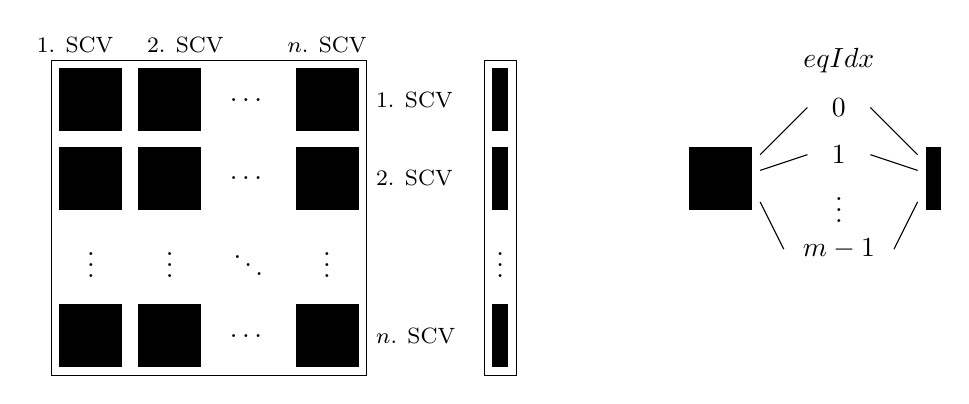
\begin{tikzpicture}
  %% blocking structure
  % matrix
  \node at (0.3,4.2){\footnotesize 1. SCV};
  \node at (1.7,4.2){\footnotesize 2. SCV};
  \node at (3.5,4.2){\footnotesize $n$. SCV};

  \draw (0,0) rectangle (4,4);
  
  \fill (0.1,3.1) rectangle (0.9,3.9);
  \fill (1.1,3.1) rectangle (1.9,3.9);
  \node at (2.5,3.5) {$\dots$};
  \fill (3.1,3.1) rectangle (3.9,3.9);
  \node at (4,3.5) [right]{\footnotesize 1. SCV};

  \fill (0.1,2.1) rectangle (0.9,2.9);
  \fill (1.1,2.1) rectangle (1.9,2.9);
  \node at (2.5,2.5) {$\dots$};
  \fill (3.1,2.1) rectangle (3.9,2.9);
  \node at (4,2.5) [right]{\footnotesize 2. SCV};

  \node at (0.5,1.5) {$\vdots$};
  \node at (1.5,1.5) {$\vdots$};
  \node at (2.5,1.5) {$\ddots$};
  \node at (3.5,1.5) {$\vdots$};

  \fill (0.1,0.1) rectangle (0.9,0.9);
  \fill (1.1,0.1) rectangle (1.9,0.9);
  \node at (2.5,0.5) {$\dots$};
  \fill (3.1,0.1) rectangle (3.9,0.9);
  \node at (4,0.5) [right]{\footnotesize $n$. SCV};

  % vector
  \draw (5.5,0) rectangle (5.9,4);
  \fill (5.6,3.1) rectangle (5.8,3.9);
  \fill (5.6,2.1) rectangle (5.8,2.9);
  \node at (5.7,1.5) {$\vdots$};
  \fill (5.6,0.1) rectangle (5.8,0.9);
  
  %% intra-block structure
  \fill (8.1,2.1) rectangle (8.9,2.9);
  \draw (9,2.8) -- (9.6,3.4);
  \draw (9,2.6) -- (9.6,2.8);
  \draw (9,2.2) -- (9.3,1.6);
  
  \node at (10,4) {${eqIdx}$};
  \node at (10,3.4) {$0$};
  \node at (10,2.8) {$1$};
  \node at (10,2.2) {$\vdots$};
  \node at (10,1.6) {$m-1$};
  
  \fill (11.1,2.1) rectangle (11.3,2.9);
  \draw (11,2.8) -- (10.4,3.4);
  \draw (11,2.6) -- (10.4,2.8);
  \draw (11,2.2) -- (10.7,1.6);
\end{tikzpicture}
\end{center}
\caption{Structure of matrix and vector, left blocking structure, right within block}
\end{figure}

Accessing entries follows this structure. You can access the pressure value in the third sub-control volume in
a vector \lstinline{sol} with \lstinline{sol[2][pressureIdx]}.


\chapter{Advanced \Dumux\ -- Detailed Instructions}
This chapter contains detailed information for those who are interested
in deeper modifications of underlying \Dumux models, classes, functions, etc.
\section[The \Dumux Models]{Physical and Numerical Models Available in \Dumux}
\todo[inline]{Evtl. könnten wir das in zwei kapitel aufsplitten? Physical und numerical
 models}

\subsection{Physical and Mathematical Description}

Characteristic of compositional multiphase models is that the phases
are not only matter of a single chemical substance. Instead, their
composition in general includes several species, and for the mass transfer,
the component behavior is quite different from the phase behavior. In the following, we
give some basic definitions and assumptions that are required for the
formulation of the model concept below. As an example, we take a
three-phase three-component system water-NAPL-gas
\cite{A3:class:2002a}. The modification for other multicomponent
systems is straightforward and can be found, e.\ g., in
\cite{A3:bielinski:2006,A3:acosta:2006}.

\subsubsection{Basic Definitions and Assumptions for the Compositional
  Model Concept}
\textbf{Components:}
The term {\it component} stands for constituents of the phases which
can be associated with a unique chemical species, or, more generally, with
a group of species exploiting similar physical behavior. In this work, we
assume a water-gas-NAPL system composed of the phases water (subscript
$\text{w}$), gas ($\text{g}$), and NAPL ($\text{n}$). These phases are
composed of the components water (superscript $\text{w}$), air
($\text{a}$), and the organic contaminant ($\text{c}$) (see Fig.\
\ref{fig:phaseMassEnergyTransfer}).

\begin{figure}
  \centering
  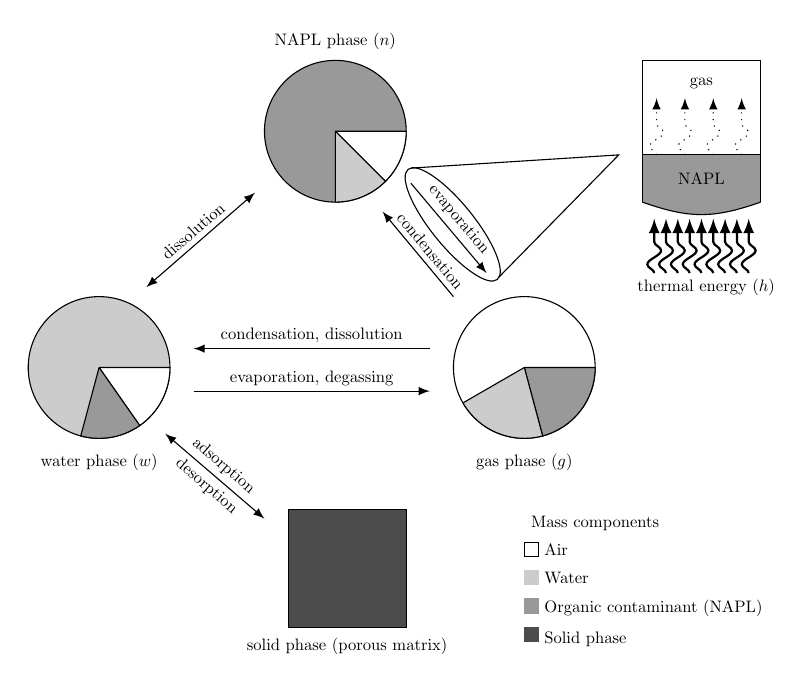
\begin{tikzpicture} [>=latex,scale=0.6, every node/.style={transform shape}]
    % Ellipse 1 solid
    \coordinate (A) at (1,-0.5);
    \draw [fill=black!70](A) rectangle(3.5,2) node at(2.25,-0.9) {solid phase (porous matrix)};
    % Ellipse 2 water
    \coordinate (B) at (-3,5);
    \draw [fill=black!20](B) circle(1.5cm);
    \node [yshift=5mm]at(-3,2.5){water phase $(w)$};
    \draw[fill=white] (B)--+(1.5,0)arc(0:-55:1.5cm)--(B);
    \draw[fill=black!40] (B)--+(-55:1.5cm)arc(-55:-105:1.5cm)--(B);
    % Ellipse 3 gas
    \coordinate (C) at (6,5);
    \draw [](C) circle (1.5cm);
    \node[yshift=5mm]at(6,2.5){gas phase $(g)$};
    \draw [fill=black!40](C)--+(1.5,0)arc(0:-75:1.5cm)--(C);
    \draw [fill=black!20] (C)--+(-75:1.5cm)arc(-75:-150:1.5cm)--(C);
    % Ellipse 4 napl
    \coordinate (D) at (2,10);
    \draw [fill=black!40](D) circle (1.5cm);
    \node[yshift=5mm]at(2,11.4){NAPL phase $(n)$};
    \draw [fill=white](D)--+(1.5,0)arc(0:-45:1.5cm)--(D);
    \draw [fill=black!20] (D)--+(0,-1.5)arc(-90:-45:1.5cm)--(D);
    % arrows
    %A-B
      \draw [<->,white](0.5,1.8)--(-1.6,3.6) node[black,above,sloped,pos=0.5]{adsorption};
      \draw [<->](0.5,1.8)--(-1.6,3.6) node[below,sloped,pos=0.5]{desorption};
    %B-C
      \draw[<-](-1,5.4)--(4,5.4)node[above,sloped,pos=0.5]{condensation, dissolution};
      \draw[->](-1,4.5)--(4,4.5)node[above,sloped,pos=0.5]{evaporation, degassing};
    %B-D
      \draw[<->](-2,6.7)--(0.3,8.7)node[above,sloped,pos=0.5]{dissolution};
    %D-C
      \draw[->](3.6,8.9)--(5.2,7)node[above,sloped,pos=0.5]{evaporation};
      \draw[rotate around={-51:(4,6.8)}](3.35,7.95) ellipse (1.5cm and 0.45cm);  %Ellipse um evaporation
      \draw (3.6,9.22)--(8,9.5)--(5.45,6.9);
      \draw[<-](3,8.3)--(4.5,6.5)node[above,sloped,pos=0.55]{condensation};
    % thermal energy
    \filldraw [black!40](8.5,9.5)rectangle(11,8.5);
    \draw (8.5,9.5)rectangle(11,11.5);
    \draw (8.5,9.5)--(8.5,8.5);
    \draw (11,9.5)--(11,8.5);
    \draw [decorate,decoration={bent,aspect=0.4,amplitude=6},fill=black!40](11,8.5)--(8.5,8.5);
    \foreach \x in {8.75,9,...,10.8}
    \draw [->,decorate,decoration={snake,post length=2mm},thick](\x,7)--(\x,8.15);
    \foreach \x in {8.8,9.4,10,10.6}
    \draw [->,dotted,decorate,decoration={snake,post length=2mm}](\x,9.5)--(\x,10.7);
    \node at(9.75,11){gas};
    \node at(9.75,9){NAPL};
    \node at(9.85,6.7){thermal energy $(h)$};
    % legende
    \node at (7.5,1.7){Mass components};
    \draw[](6,1)rectangle +(0.3,0.3) node at(6.3,1.15) [right]{Air};
    \filldraw[black!20](6,0.4) rectangle +(0.3,0.3) node at (6.3,0.55)[black,right]{Water};
    \filldraw[black!40](6,-0.2) rectangle +(0.3,0.3) node at (6.3,-0.1)[right,black]{Organic contaminant (NAPL)};
    \filldraw[black!70](6,-0.8) rectangle +(0.3,0.3) node at (6.3,-0.75)[right,black]{Solid phase};
  \end{tikzpicture}
  \caption{Mass and energy transfer between the phases}
  \label{fig:phaseMassEnergyTransfer}
\end{figure}

\textbf{Equilibrium:}
For the non-isothermal multiphase processes in porous media under
consideration, we state that the assumption of local thermal
equilibrium is valid since flow velocities are small. We neglect
chemical reactions and biological decomposition and assume chemical
equilibrium.  Mechanical equilibrium is not valid in a porous medium,
since discontinuities in pressure can occur across a fluid-fluid
interface due to capillary effects.

\textbf{Notation:} The index $\alpha \in \{\text{w}, \text{n}, \text{g}\}$ refers
to the phase, while the superscript $\kappa \in \{\text{w}, \text{a}, \text{c}\}$ refers
to the component. \\
\begin{tabular}{llll}
$p_\alpha$ & phase pressure & $\phi$ & porosity \\
$T$ & temperature & $K$ & absolute permeability tensor \\
$S_\alpha$ & phase saturation & $\tau$ & tortuosity \\
$x_\alpha^\kappa$ & mole fraction of component $\kappa$ in phase $\alpha$ & $\boldsymbol{g}$ & gravitational acceleration \\
$X_\alpha^\kappa$ & mass fraction of component $\kappa$ in phase $\alpha$ & $q^\kappa_\alpha$ & volume source term of $\kappa$ in $\alpha$ \\
$\varrho_{\text{mol},\alpha}$ & molar density of phase $\alpha$ & $u_\alpha$ & specific internal energy \\
$\varrho_{\alpha}$ & mass density of phase $\alpha$ & $h_\alpha$ & specific enthalpy \\
$M$ & molar mass of a phase or component & $c_\text{s}$ & specific heat enthalpy \\
$k_{\text{r}\alpha}$ & relative permeability & $\lambda_\text{pm}$ & heat conductivity \\
$\mu_\alpha$ & phase viscosity & $q^h$ & heat source term \\
$D_\alpha^\kappa$ & diffusivity of component $\kappa$ in phase $\alpha$ & $\boldsymbol{v}_{a,\alpha}$  & advective velocity \\
$\boldsymbol{v}_\alpha$ & velocity (Darcy or free flow)& & \\
\end{tabular}


\subsubsection{Balance Equations}
For the balance equations for multicomponent systems, it is in many
cases convenient to use a molar formulation of the continuity
equation. Considering the mass conservation for each component allows
us to drop source/sink terms for describing the mass transfer between
phases. Then, the
molar mass balance can be written as:
%
\begin{multline}
  \label{A3:eqmass1}
 \phi \frac{\partial (\sum_\alpha \varrho_{\text{mol}, \alpha}
    x_\alpha^\kappa S_\alpha )}{\partial t}
 - \sum\limits_\alpha \Div \left\lbrace \frac{k_{\text{r}
        \alpha}}{\mu_\alpha} \varrho_{\text{mol}, \alpha}
    x_\alpha^\kappa \textbf{K} (\grad p_\alpha -
    \varrho_{\alpha} \boldsymbol{g}) \right\rbrace  \\
  %
  %
 - \sum\limits_\alpha \Div \left\lbrace \tau \phi S_\alpha D_\alpha^\kappa \varrho_{\text{mol},
      \alpha} \grad x_\alpha^\kappa \right\rbrace
 - q^\kappa = 0, \qquad \kappa \in \{\text{w,a,c}\}.
\end{multline}

The component mass balance can also be written in terms of mass fractions
by replacing molar densities by mass densities and mole by mass fractions.
To obtain a single conserved quantity in the temporal derivative, the total
concentration, representing the mass of one component per unit volume, is defined as
\begin{displaymath}
C^\kappa = \sum_\alpha \phi S_\alpha \varrho_{\text{mass},\alpha} X_\alpha^\kappa \; .
\end{displaymath}
Using this definition, the component mass balance is written as:

\begin{multline}
  \label{A3:eqmass2}
    \frac{\partial C^\kappa}{\partial t} =
  \sum\limits_\alpha \Div \left\lbrace \frac{k_{\text{r}
        \alpha}}{\mu_\alpha} \varrho_{\text{mass}, \alpha}
    X_\alpha^\kappa \textbf{K} (\grad p_\alpha +
    \varrho_{\text{mass}, \alpha} \boldsymbol{g}) \right\rbrace  \\
  %
  %
   + \sum\limits_\alpha \Div \left\lbrace \tau \phi S_\alpha D_\alpha^\kappa \varrho_{\text{mass},
      \alpha} \frac{M^\kappa}{M_\alpha} \grad x_\alpha^\kappa \right\rbrace
 + q^\kappa = 0, \qquad \kappa \in \{\text{w,a,c}\}.
\end{multline}


In the case of non-isothermal systems, we further have to balance the
thermal energy. We assume fully reversible processes, such that entropy
is not needed as a model parameter. Furthermore, we neglect
dissipative effects and the heat transport due to molecular
diffusion. The energy balance can then be
formulated as:
%
\begin{multline}
  \label{A3:eqenergmak1}
  \phi \frac{\partial \left( \sum_\alpha \varrho_{\alpha}
      u_\alpha S_\alpha \right)}{\partial t} + \left( 1 -
    \phi \right) \frac{\partial \varrho_{\text{s}} c_{\text{s}}
    T}{\partial t}
 - \Div \left( \lambda_{\text{pm}} \grad T \right)
   \\
   - \sum\limits_\alpha \Div \left\lbrace \frac{k_{\text{r}
        \alpha}}{\mu_\alpha} \varrho_{\alpha} h_\alpha
    K \left( \grad p_\alpha - \varrho_{\alpha}
      \boldsymbol{g} \right) \right\rbrace
 - q^h \; = \; 0.
\end{multline}

In order to close the system, supplementary constraints for capillary pressure, saturations and mole
fractions are needed, \cite{A3:helmig:1997}.
According to the Gibbsian phase rule, the number of degrees of freedom
in a non-isothermal compositional multiphase system is equal to the
number of components plus one. This means we need as many independent
unknowns in the system description. The
available primary variables are, e.\ g., saturations, mole/mass
fractions, temperature, pressures, etc.

\subsection{Available Models}
The following description of the available models is automatically extracted
from the Doxygen documentation.

\todo[inline]{Die Modelle waren etwas uneinheitlich von der Notation (ich habe
  hier auch gerade das entsprechende ToDo entfernt). Das ist naturlich jetzt
  nicht mehr so schlimm, da die Modelle nicht mehr untereinander auftauchen,
  allerdings wird auch die Fehlersuche schwieriger (aus dem Auge aus dem Sinn).}

\todo[inline]{evtl. entferne Unterkapitel. Einfugen der Modelliste, die könnte
  in ahnlicher Form auch aufs doxygen? Update der Liste in die Release Manager
  Tasks ubernehmen}

\subsubsection{Fully-Implicit Models}

The fully-implicit models described in this section are using the box or the
cell centered finite volume method as described in section \ref{box} and \ref{cc}
for spatial and the implicit Euler
method as temporal discretization. The models themselves are located in
subdirectories of \texttt{dumux/implicit} of the \Dumux distribution.

\subsubsection{Decoupled Models}
%
The basic idea the so-called decoupled models have in common is to reformulate the
equations of multi-phase flow (e.g. Eq. \ref{A3:eqmass1}) into one equation for
pressure and equations for phase-/component-/etc. transport. The pressure equation
is the sum of the mass balance equations and thus considers the total flow of the
fluid system. The new set of equations is considered as decoupled (or weakly coupled)
and can thus be solved sequentially. The most popular decoupled model is the so-called
fractional flow formulation for two-phase flow which is usually implemented applying
an IMplicit Pressure Explicit Saturation algorithm (IMPES).
In comparison to a fully implicit model, the decoupled structure allows the use of
different discretization methods for the different equations. The standard method
used in the decoupled models is a cell centered finite volume method. Further schemes,
so far only available for the two-phase pressure equation, are cell centered finite
volumes with multi-point flux approximation (MPFA O-method) and mimetic finite differences.

An $h$-adaptive implementation of both decoupled models is provided for two dimensions.

\section{Spatial Discretization Schemes}
\label{spatialdiscretization}

We discretize space with the cell-centered finite volume method (\ref{cc} ), the box method (\ref{box})
or a staggered grid scheme.
Grid adaption is available for both box and cell-centered finite volume method.
In general, the spatial  parameters, especially the porosity, have to be assigned on
the coarsest level of discretization.

\subsection{Box Method -- A Short Introduction}\label{box}

The so called box method unites the advantages of the finite-volume (FV) and
finite-element (FE) methods.

First, the model domain $\Omega$ is discretized with a FE mesh consisting of nodes
$i$ and corresponding elements $E_k$. Then, a secondary FV mesh is constructed
by connecting the midpoints and barycenters of the elements surrounding node
$i$ creating a box $B_i$ around node $i$ (see Figure \ref{pc:box}a).

\begin{figure} [ht]
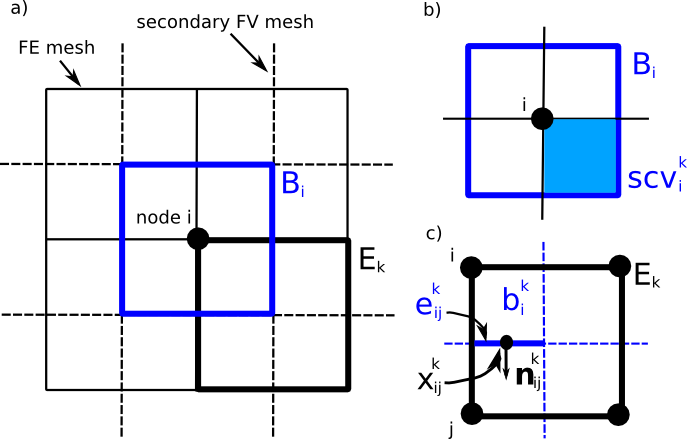
\includegraphics[width=0.8\linewidth,keepaspectratio]{png/box_disc.png}
\caption{\label{pc:box} Discretization of the box method}
\end{figure}

The FE mesh divides the box $B_i$ into subcontrolvolumes (scv's) $b^k_i$
(see Figure \ref{pc:box}b). Figure \ref{pc:box}c shows the finite element $E_k$
and the scv's $b^k_i$ inside $E_k$, which belong to four different boxes $B_i$.
Also necessary for the discretization are the faces of the subcontrolvolumes (scvf's)
$e^k_{ij}$ between the scv's $b^k_i$ and $b^k_j$, where $|e^k_{ij}|$ is the length
of the scvf. The integration points $x^k_{ij}$ on $e^k_{ij}$ and the outer normal
vector $\mathbf n^k_{ij}$ are also to be defined (see Figure \ref{pc:box}c).

The advantage of the FE method is that unstructured grids can be used, while the
FV method is mass conservative. The idea is to apply the FV method (balance of
fluxes across the interfaces) to each FV box $B_i$  and to get the fluxes across
the interfaces $e^k_{ij}$ at the integration points $x^k_{ij}$ from the FE approach.
Consequently, at each scvf the following expression results:

\begin{equation}
 	f(\tilde u(x^k_{ij})) \cdot \mathbf n^k_{ij} \: |e^k_{ij}| \qquad \textrm{with}
 	\qquad \tilde u(x^k_{ij}) = \sum_i N_i(x^k_{ij}) \cdot \hat u_i .
\end{equation}

In the following, the discretization of the balance equation is going to be derived.
From the \textsc{Reynolds} transport theorem follows the general balance equation:

\begin{equation}
	\underbrace{\int_\Omega \frac{\partial}{\partial t} \: u \: dx}_{1}
	+ \underbrace{\int_{\partial\Omega} (\mathbf{v} u + \mathbf w) \cdot \textbf n \: d\varGamma}_{2} = \underbrace{\int_\Omega q \: dx}_{3}
\end{equation}

\begin{equation}
	f(u) = \int_\Omega \frac{\partial u}{\partial t} \: dx + \int_{\Omega} \nabla \cdot
	\underbrace{\left[  \mathbf{v} u + \mathbf w(u)\right] }_{F(u)}  \: dx - \int_\Omega q \: dx = 0
\end{equation}
where term 1 describes the changes of entity $u$ within a control volume over
time, term 2 the advective, diffusive and dispersive fluxes over the interfaces
of the control volume and term 3 is the source and sink term. $\Omega$ denotes the
model domain and $F(u) = F(\mathbf v, p) = F(\mathbf v(x,t), p(x,t))$.

Like the FE method, the box method follows the principle of weighted residuals.
In the function $f(u)$ the unknown $u$ is approximated by discrete values at the
nodes of the FE mesh $\hat u_i$ and linear basis functions $N_i$ yielding an
approximate function $f(\tilde u)$. For $u\in \lbrace \mathbf v, p, x^\kappa \rbrace$
this means:

\begin{minipage}[b]{0.47\textwidth}
\begin{equation}
\label{eq:p}
	\tilde p = \sum_i N_i \hat{p}_i
\end{equation}
\begin{equation}
\label{eq:v}
	\tilde{\mathbf v} = \sum_i N_i \hat{\mathbf v}_i
\end{equation}
\begin{equation}
\label{eq:x}
	\tilde x^\kappa  = \sum_i N_i \hat x_i^\kappa
\end{equation}
\end{minipage}
\hfill
\begin{minipage}[b]{0.47\textwidth}
\begin{equation}
\label{eq:dp}
	\nabla \tilde p = \sum_i \nabla N_i \hat{p}_i
\end{equation}
\begin{equation}
\label{eq:dv}
	\nabla \tilde{\mathbf v} = \sum_i \nabla N_i \hat{\mathbf v}_i
\end{equation}
\begin{equation}
\label{eq:dx}
	\nabla \tilde x^\kappa  = \sum_i \nabla N_i \hat x_i^\kappa .
\end{equation}
\end{minipage}

Due to the approximation with node values and basis functions the differential
equations are not exactly fulfilled anymore but a residual $\varepsilon$ is produced.

\begin{equation}
	f(u) = 0  \qquad \Rightarrow \qquad f(\tilde u) = \varepsilon
\end{equation}

Application of the principle of weighted residuals, meaning the multiplication
of the residual $\varepsilon$ with a weighting function $W_j$  and claiming that
this product has to vanish within the whole domain,

\begin{equation}
	\int_\Omega W_j \cdot \varepsilon \: \overset {!}{=} \: 0 \qquad \textrm{with} \qquad \sum_j W_j =1
\end{equation}
yields the following equation:

\begin{equation}
	\int_\Omega W_j \frac{\partial \tilde u}{\partial t} \: dx + \int_\Omega W_j
	\cdot \left[ \nabla \cdot F(\tilde u) \right]  \: dx - \int_\Omega W_j
	\cdot q \: dx = \int_\Omega W_j \cdot \varepsilon \: dx \: \overset {!}{=} \: 0.	
\label{eq:weightedResidual}	
\end{equation}

For standard Galerkin schemes, the weighting functions $W_j$ are chosen the same as the ansatz functions $N_j$. However, this does not yield a locally mass-conservative scheme. 
Therefore, for the Box method, the weighting functions $W_j$ are chosen as 
the piecewise constant functions over a
control volume box $B_j$, i.e.

\begin{equation}
	W_j(x) = \begin{cases}
	          1 &x \in B_j \\
		  0 &x \notin B_j.\\
	         \end{cases}
\label{eq:weightingFunctions}	         
\end{equation}
Thus, the Box method is a Petrov-Galerkin scheme, where the weighting functions do not belong to the same function space than the ansatz functions.

Inserting definition \eqref{eq:weightingFunctions} into equation \eqref{eq:weightedResidual} and using the \textsc{Green-Gaussian} integral theorem results in
\begin{equation}
	\int_{B_j} \frac{\partial \tilde u}{\partial t} \: dx + \int_{\partial B_j}  F(\tilde u) \cdot \mathbf n \: d\varGamma_{B_j} - \int_{B_j} q \: dx  \overset {!}{=} \: 0, 	
\label{eq:BoxMassBlance}	
\end{equation}
which has to hold for every box $B_j$. 

The first term in equation \eqref{eq:BoxMassBlance} can be written as
\begin{equation}
\int_{B_j} \frac{\partial \tilde u}{\partial t} \: dx = \frac{d}{dt} \int_{B_j} \sum_i \hat u_i N_i  \: dx = \sum_i \frac{\partial \hat u_i}{\partial t} \int_{B_j}  N_i  \: dx.
\end{equation} 
Here, a mass lumping technique is applied by assuming that the storage capacity is
reduced to the nodes. This means that the integrals $M_{i,j} = \int_{B_j}  N_i \: dx$
are replaced by some mass lumped terms $M^{lump}_{i,j}$ which are defined as
\begin{equation}
	 M^{lump}_{i,j} =\begin{cases}  V_j &j = i\\
	0 &j \neq i,\\
	         \end{cases}
\end{equation}
where $V_j$ is the volume of the FV box $B_j$ associated with node $j$.
The application of this assumption yields

\begin{equation}
\label{eq:disc1}
	V_j \frac{\partial \hat u_j}{\partial t}
	+  \int_{\partial B_j}  F(\tilde u) \cdot \mathbf n \: d\varGamma_{B_j} - Q_j = 0,
\end{equation}
where $Q_j$ is an approximation (using some quadrature rule) of the integrated source/sink term $\int_{B_j} q \: dx$.

Using an implicit Euler time discretization finally
leads to the discretized form which will be applied to the mathematical
flow and transport equations:

\begin{equation}
\label{eq:discfin}
	V_j \frac{\hat u_j^{n+1} - \hat u_j^{n}}{\Delta t}
	+ \int_{\partial B_j}  F(\tilde u^{n+1}) \cdot \mathbf n
	\;  d{\varGamma}_{B_j} - Q_j^{n+1} \: = 0.
\end{equation}
Equation \eqref{eq:discfin} has to be fulfilled for each box $B_j$.

\subsection{Cell Centered Finite Volume Methods -- A Short Introduction}\label{cc}
Cell-centered finite volume methods use the elements of the grid as control volumes.
For each control volume the discrete values are determined at the element/control
volume center (not required to be the barycenters). 

We consider a domain $\Omega \subset \mathbb{R}^d$, $d \in \{ 2, 3 \}$ with boundary $\Gamma = \partial \Omega$. Within this section, we consider the following elliptic problem
\begin{equation}
  \begin{aligned}
                   \nabla \cdot \left( - \mathbf{\Lambda} \nabla u \right) &= q   &&\mathrm{in} \, \Omega \\
               \left( - \mathbf{\Lambda} \nabla u \right) \cdot \mathbf{n} &= v_N &&\mathrm{on} \, \Gamma_N \\
                                                                   u &= u_D &&\mathrm{on} \, \Gamma_D.
    \label{eq:elliptic}
  \end{aligned}
\end{equation}

Here, $\mathbf{\Lambda} = \mathbf{\Lambda}(\mathbf{x}, \mathbf{u})$ is a symmetric and positive definite tensor of second rank (e.g. permeability, diffusivity, etc.), $u = u (\mathbf{x})$ is unknown and $q = q(\mathbf{x}, \mathbf{u})$ is a source/sink. 
We denote by $\mathcal{M}$ the mesh that results from the division of the domain $\Omega$ into $n_e$ control volumes $K \subset \Omega$. Each $K$ is a polygonal open set such that $K \cap L = \emptyset, \forall{K \neq L}$ and $\overline{\Omega} = \cup_{K \in \mathcal{M}} \overline{K}$. 

For the derivation of the finite-volume formulation we integrate the first equation of \eqref{eq:elliptic} over a control volume $K$ and apply the Gauss divergence theorem:

\begin{equation}
    \int_{\partial K} \left( - \mathbf{\Lambda} \nabla u \right) \cdot \mathbf{n} \, \mathrm{d} \Gamma = \int_K q \, \mathrm{d}\Omega.
    \label{eq:ellipticIntegrated}
\end{equation}

Splitting the control volume boundary $\partial K$ into a finite number of faces $\sigma \subset \partial K$ (such that $\sigma = \overline{K} \cap \overline{L}$ for some neighboring control volume $L$) and replacing the exact fluxes by an approximation, i.e. $F_{K, \sigma} \approx \int_{\sigma} \left( - \mathbf{\Lambda} \nabla u \right) \cdot \mathbf{n} \mathrm{d} \Gamma$, yield
\begin{equation}
    \sum_{\sigma \subset \partial K} F_{K, \sigma} = Q_K, \quad \forall \, {K \in \mathcal{M}},
\label{eq:ccdisc}
\end{equation}
where $F_{K, \sigma}$ is the discrete flux through face $\sigma$ flowing out of cell $K$ and $Q_K := \int_K q \, \mathrm{d}x$ is the integrated source/sink term. Equation \eqref{eq:ccdisc} is the typical cell-centered finite-volume formulation. 
Finite-volume schemes differ in the way how the term 
$(\mathbf{\Lambda} \nabla u ) \cdot \mathbf{n} $ is approximated (i.e. the choice of the fluxes $F_{K, \sigma}$). Using the symmetry of the tensor $\mathbf{\Lambda}$, this term can be rewritten as 
$\nabla u  \cdot \mathbf{\Lambda}\mathbf{n}$, which corresponds to the directional derivative of $u$ in co-normal direction $\mathbf{\Lambda}\mathbf{n}$. 
In the following, the main ideas of the two-point flux approximation and the multi-point flux approximation methods are briefly described. Hereby, we restrict the discussion to the two-dimensional case.

Please also note that other types of equations, e.g. instationary parabolic problems, can be discretized by applying some time discretization scheme to the time derivatives and by using the finite-volume scheme for the flux discretization. For simplicity the discussion is restricted to the elliptic problem \eqref{eq:elliptic}.

\subsubsection{Tpfa Method}\label{cc_tpfa}
The linear two-point flux approximation is a simple but robust cell-centered finite-volume scheme, which is commonly used in commercial software. 
This scheme can be derived by using the conormal decomposition, which reads
\begin{equation}
\mathbf{\Lambda}_K \mathbf{n}_{K, \sigma} = t_{K,\sigma} \mathbf{d}_{K,\sigma} + \mathbf{d}^{\bot}_{K,\sigma}, \quad  t_{K,\sigma} = \frac{\mathbf{n}_{K, \sigma}^T \mathbf{\Lambda}_K \mathbf{d}_{K,\sigma} }{\mathbf{d}_{K,\sigma}^T \mathbf{d}_{K,\sigma}}, \; \mathbf{d}^{\bot}_{K,\sigma} = \mathbf{\Lambda}_K \mathbf{n}_{K, \sigma} - t_{K,\sigma} \mathbf{d}_{K,\sigma},
\label{eq:conormalDecTpfa}
\end{equation}
with the distance vector $\mathbf{d}_{K,\sigma} := \mathbf{x}_\sigma - \mathbf{x}_K$ and $\mathbf{d}_{K,\sigma}^T \mathbf{d}^{\bot}_{K,\sigma} = 0$, see Figure \ref{pc:cctpfa} for the used notations. The same can be done for the conormal $\mathbf{\Lambda}_L \mathbf{n}_{L, \sigma}$. The $t_{K,\sigma}$ and $t_{L,\sigma}$ are the transmissibilities associated with the face $\sigma$. These transmissibilities are calculated in \Dumux by using the function \texttt{computeTpfaTransmissibility}.

\begin{figure} [ht]
\centering

\includegraphics[width=0.4\linewidth,keepaspectratio]{PNG/cctpfa.png}
\caption{Two neighboring control volumes sharing the face $\sigma$.}
\label{pc:cctpfa}
\end{figure}


With these notations, it follows that for each cell $K$ and face $\sigma$ 
\begin{equation}
\nabla u \cdot \mathbf{\Lambda}_K \mathbf{n}_{K, \sigma} =  t_{K,\sigma} \nabla u \cdot \mathbf{d}_{K,\sigma} + \nabla u \cdot \mathbf{d}^{\bot}_{K,\sigma}.
\end{equation}
For the Tpfa scheme, the second part in the above equation is neglected. By using the fact that $\nabla u \cdot \mathbf{d}_{K,\sigma} \approx u_\sigma - u_K$, the discrete fluxes for face $\sigma$ are given by
\begin{equation}
F_{K,\sigma} = -\meas{\sigma}  t_{K,\sigma} (u_\sigma - u_K), \qquad F_{L,\sigma} = -\meas{\sigma}  t_{L,\sigma} (u_\sigma - u_L).
\label{eq:TPFAOneSided}
\end{equation}
Enforcing local flux conservation, i.e. $F_{K,\sigma}+F_{L,\sigma}=0$, results in 
\begin{equation}
u_\sigma = \frac{t_{K,\sigma} u_K + t_{L,\sigma} u_L}{t_{K,\sigma}  + t_{L,\sigma}}.
\end{equation}
With this, the fluxes \eqref{eq:TPFAOneSided} are rewritten as
\begin{equation}
F_{K,\sigma} = \meas{\sigma}  \frac{t_{K,\sigma} t_{L,\sigma}}{t_{K,\sigma} + t_{L,\sigma}} (u_K - u_L), \quad F_{L,\sigma} = \meas{\sigma}  \frac{t_{K,\sigma} t_{L,\sigma}}{t_{K,\sigma} + t_{L,\sigma}} (u_L - u_K).
\label{eq:TPFAFlux}
\end{equation}
By neglecting the orthogonal term, the consistency of the scheme is lost for general grids, where $\nabla u \cdot \mathbf{d}^{\bot}_{K,\sigma} \not = 0$. The consistency is achieved only for so-called K-orthogonal grids for which $\mathbf{d}^{\bot}_{K,\sigma} = 0$. For such grids we deduce that 
\begin{equation}
\frac{t_{K,\sigma} t_{L,\sigma}}{t_{K,\sigma} + t_{L,\sigma}} = \frac{\tau_{K,\sigma} \tau_{L,\sigma}}{\tau_{K,\sigma} d_{L,\sigma} + \tau_{L,\sigma} d_{K,\sigma}},
\label{eq:TPFAcoeffNew}
\end{equation}
with $\tau_{K,\sigma} := \mathbf{n}_{K, \sigma} \mathbf{\Lambda}_K\mathbf{n}_{K, \sigma}, \tau_{L,\sigma} := \mathbf{n}_{L, \sigma} \mathbf{\Lambda}_L\mathbf{n}_{L, \sigma}$, $d_{K,\sigma}:= \mathbf{n}_{K, \sigma} \cdot \mathbf{d}_{K, \sigma}$, and $d_{L,\sigma}:= \mathbf{n}_{L, \sigma} \cdot \mathbf{d}_{L, \sigma}$. This reduces, for the case of scalar permeability, to a distance weighted harmonic averaging of permeabilities.

 

\subsubsection{Mpfa Method}\label{cc_mpfa}
Expressions for the face fluxes $F_{K, \sigma}$ are usually obtained by introducing intermediate face unknowns $u_\sigma$ in addition to the cell unknowns $u_K$ and enforcing the physically motivated continuity of fluxes and continuity of the solution across the faces. For a face $\sigma$ between the two polygons $K$ and $L$ these conditions read:
\begin{equation}
    \begin{aligned}
        &F_{K, \sigma} + F_{L, \sigma} = 0 \\
        &{u}_{K,\sigma} = {u}_{L,\sigma} = {u}_{\sigma}.
        \label{eq:sigmaConditions}
    \end{aligned}
\end{equation}
Using these conditions the intermediate face unknowns ${u}_\sigma$ can be eliminated and the fluxes are expressed as a function of the cell unknowns $u_N$ and associated transmissibilities $t^N_{K,\sigma}$:

\begin{equation}
    F_{K,\sigma} = \sum_{N \in \mathcal{S}_{K,\sigma}} t^N_{K,\sigma} u_{N}.
    \label{eq:FVFluxExpression}
\end{equation}

\begin{figure} [ht]
\centering
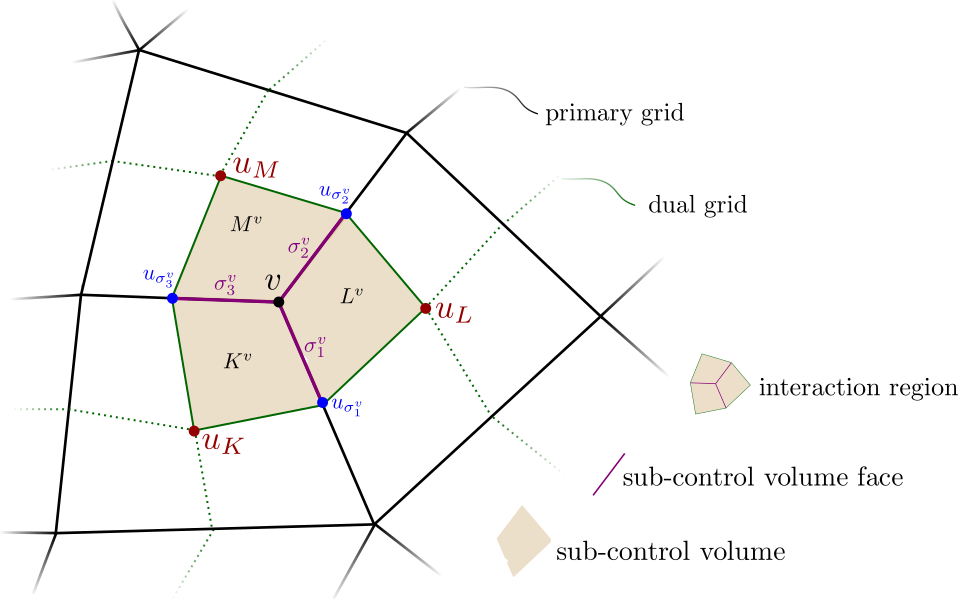
\includegraphics[width=0.8\linewidth,keepaspectratio]{PNG/mpfa_iv.png}
\caption{Interaction region for the Mpfa-O method. The graphic on the right illustrates how the sub-control volume $L^v$ and face $\sigma^v_2$ are embedded in cell $L$. Note that the face stencils for all sub-control volume faces in the depicted interaction region are $\mathcal{S}_{\sigma^v_i} = \{ K,L,M \}$, meaning that the fluxes over the sub-control volume faces depend on the three cell unknowns $u_K, u_L, u_M$.}
\label{pc:interactionRegion_mpfa}
\end{figure}

The main difference between the various finite-volume schemes available is the assembly of the face fluxes, i.e. the computation of the $t^N_{K,\sigma}$ and the size of $\mathcal{S}_{K,\sigma}$. For the Tpfa, that has been presented in the last section, the stencil and transmissibilities are given as
\begin{equation*}
\mathcal{S}_{K,\sigma} = \lbrace K,L \rbrace, \quad t^K_{K,\sigma} =  \meas{\sigma}  \frac{t_{K,\sigma} t_{L,\sigma}}{t_{K,\sigma} + t_{L,\sigma}},\; t^L_{K,\sigma} =  -\meas{\sigma}  \frac{t_{K,\sigma} t_{L,\sigma}}{t_{K,\sigma} + t_{L,\sigma}},
\end{equation*}
with $t_{K,\sigma},t_{L,\sigma}$ as defined in equation \eqref{eq:conormalDecTpfa}.

In the following, a multi-point flux approximation method (Mpfa-O method), which was first introduced in \citet{Aavatsmark2002}, is presented. The main difference to the Tpfa scheme is the fact that a consistent discrete gradient is constructed, i.e. the term $\nabla u \cdot \mathbf{d}^{\bot}_{K,\sigma}$ is not neglected.

For this scheme, a dual grid is created by connecting the barycenters of the cells with the barycenters of the faces ($d=2$) or the barycenters of the faces and edges ($d=3$). This divides each cell into sub-control volumes $K^v$. Analogously, each face is sub-divided into sub-control volume faces $\sigma^v$, see Figure \ref{pc:interactionRegion_mpfa}. We allow for piecewise constant $\mathbf{\Lambda}$ (per cell) and construct discrete gradients $\nabla_\mathcal{D}^{K^v} u$ (per sub-control volume $K^v$). 
In the following, we restrict our discussion to the two-dimensional setup that is shown in Figure \ref{pc:interactionRegion_mpfa}.  
Here, the discrete gradients are constructed to be consistent such that the following conditions hold:
\begin{equation}
\nabla_\mathcal{D}^{K^v} u \cdot (\mathbf{x}_{\sigma^v_1}- \mathbf{x}_{K}) = u_{\sigma^v_1} - u_K, \quad \nabla_\mathcal{D}^{K^v} u \cdot (\mathbf{x}_{\sigma^v_3}- \mathbf{x}_{K}) = u_{\sigma^v_3} - u_K.
\end{equation}
Thus, a discrete gradient (for sub-control volume $K^v$) that fulfills  these conditions is given as
\begin{equation}
\nabla_\mathcal{D}^{K^v} u  = \mathbb{D}^{-T}_{K^v}
 \begin{bmatrix}
  u_{\sigma^v_1} - u_K \\
  u_{\sigma^v_3} - u_K
 \end{bmatrix}, \qquad \text{ with }\; \mathbb{D}_{K^v} := 
  \begin{bmatrix}
   \mathbf{x}_{\sigma^v_1}- \mathbf{x}_K & \mathbf{x}_{\sigma^v_3} - \mathbf{x}_K
 \end{bmatrix}.
 \label{eq:MPFAGradientRecons}
\end{equation}

This enables us to write the discrete flux across $\sigma^v_1$ from cell $K$ as follows:
\begin{equation}
    F_{K, \sigma^v_1} := - |\sigma^v_1| \mathbf{n}_{\sigma^v_1}^T \mathbf{\Lambda}_K \nabla_\mathcal{D}^{K^v} u.
    \label{eq:discreteFlux}
\end{equation}
Inserting the discrete gradient, yields
\begin{equation}
    F_{K, \sigma^v_1} = \omega_{K,\sigma^v_1\sigma^v_1}(u_K - u_{\sigma^v_1}) + \omega_{K,\sigma^v_1 \sigma^v_3}(u_K - u_{\sigma^v_3}),
    \label{eq:discreteFluxRef}
\end{equation}
with $(\omega_{K,\sigma^v_1\sigma^v_1},\omega_{K,\sigma^v_1 \sigma^v_3})^T = |\sigma^v_1| \mathbb{D}^{-1}_{K^v}\mathbf{\Lambda}_K \mathbf{n}_{\sigma^v_1}$. 
\\ \ \\
To deduce a cell-centered scheme, the introduced face unknowns $u_{\sigma^v_i}$ have to be eliminated. This is done by enforcing flux continuity for each sub-control volume face, i.e.
\begin{align}
F_{K, \sigma^v_1} + F_{L, \sigma^v_1} &= 0, \\ F_{K, \sigma^v_3} + F_{M, \sigma^v_3} &= 0, \\ F_{L, \sigma^v_2} + F_{M, \sigma^v_2} &= 0.
\end{align}
This results in a system of equations for the face unknowns $\mathbf{u}_{\sigma}$
\begin{equation}
\mathbb{A}^{3\times 3} \mathbf{u}_{\sigma} = \mathbb{B}^{3\times 3} \mathbf{u},
\end{equation}
where $\mathbf{u}$ contains the three cell unknowns $u_K,u_L,u_M$ and $\mathbf{u}_{\sigma}$ the three face unknowns $u_{\sigma^v_1}, u_{\sigma^v_2}, u_{\sigma^v_3}$. 
Inserting these face unknowns into the flux expression \eqref{eq:discreteFluxRef} yields
\begin{equation}
    F_{K,\sigma^v_i} = \sum_{N \in \lbrace K,L,M \rbrace } t^N_{K,\sigma^v_i} u_{N} = \mathbf{t}_{K,\sigma^v_i} \cdot \mathbf{u},
    \label{eq:FVFluxExpressionSubFace}
\end{equation}
for each cell $K$ and sub-control volume face $\sigma^v_i$. 
In \Dumux the transmissibility vector $\mathbf{t}_{K,\sigma^v_i}$ is returned by the function \texttt{advectionTijSecondaryIv()} or \texttt{advectionTijPrimaryIv()}, depending on the chosen interaction volume type (the primary interaction volume is used by default).

% \subsubsection{NLTPFA}\label{cc_nltpfa}
% TODO

\subsection{Staggered Grid -- A Short Introduction}\label{staggered}

\begin{figure}[ht]
\centering
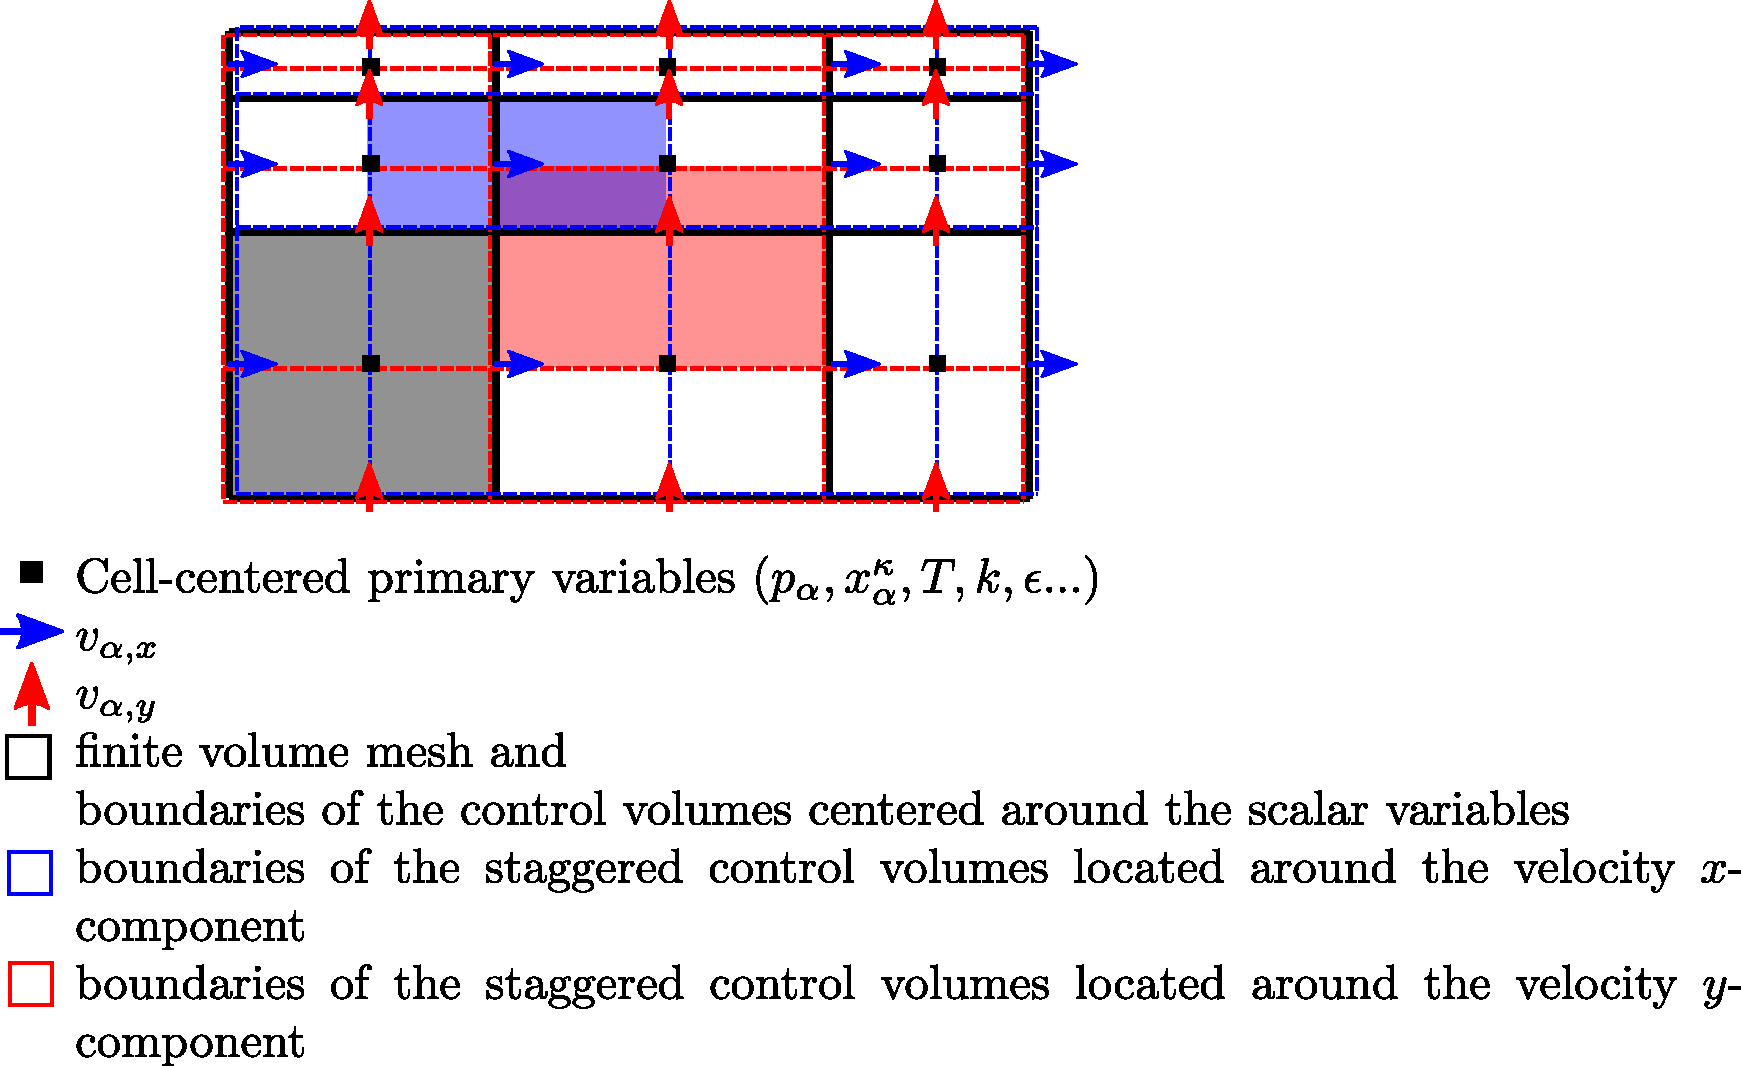
\includegraphics[width=.8\linewidth]{./pdf/staggered_grid.pdf}
\caption{\label{pc:staggered} Discretization of the staggered-grid method. The figure shows the different control volume arrangements, which are staggered with respect to each other. There are the control volumes centered around the scalar primary variables in black, the control volumes located around the $x$-component of the velocity in blue and the control volumes located around the $y$-components of the velocity in red. The control volume boundaries are given by lines. Additionally, there is one shaded example control volume each.\\
In the two-dimensional free-flow models, the continuity equation is discretized using the black control volumes, the $x$-component of the momentum equation is discretized using the blue control volumes and the $y$-component is discretized using the red control volumes. In three dimensions this works analogously.}
\end{figure}

The staggered-grid or marker-and-cell method uses a finite volume method with different control volumes for different equations. There are control volumes centered around the scalar primary variables. They correspond to the finite volume mesh. Additionally, there are control volumes located around the $x,y$ and (in 3D) $z$ velocity components which are shifted in the $x,y$ and $z$ direction, such that the velocity components are located on the edges of the cell-centered finite volume mesh (see Figure~\ref{pc:staggered}). As for the cell-centered method, the fluxes are evaluated at the edges of each control volume with a two-point flux approximation, cf. \ref{cc}.\par
The staggered-grid method is robust, mass conservative, and free of pressure oscillations
but should, as the cell-centered TPFA method, only be applied for structured grids.
Currently, all free-flow models in \Dumux use the staggered-grid discretization.

\section{Steps of a \Dumux Simulation}
\label{flow}


This chapter is supposed to give a short overview over how things are ``handed around'' in \Dumux. It
is not a comprehenisve guide through the modeling framework of \Dumux, but
hopefully it will help getting to grips with it.

In Section \ref{content} the structure of \Dumux is shown from a \emph{content}
point of view.

\subsection{Structure -- by Content}

\label{content}
In Figure \ref{fig:algorithm}, the algorithmic representations of a monolithical
solution solution scheme is illustrated down to the element level.

\begin{figure}[hbt]
\setcounter{thingCounter}{0}

\scriptsize
\sffamily
\begin{center}\parbox{0cm}{
\begin{tabbing}
\textbf{{\begin{turn}{45}\color{black}\numberThis{main}{init}\end{turn}}}             \=
\textbf{{\begin{turn}{45}\color{dumuxBlue}\numberThis{time step}{prep}\end{turn}}}            \=
\textbf{{\begin{turn}{45}\color{Mulberry}\numberThis{\textsc{Newton}}{elem}\end{turn}}}         \=
\textbf{{\begin{turn}{45}\color{dumuxYellow}\numberThis{element}{calc}\end{turn}}}             \=  \\
\\
\color{black}initialize \\
\color{black}\textbf{foreach} time step\\

  \> \color{dumuxBlue}\textbf{foreach} \textsc{Newton} iteration \\

    \> \> \color{Mulberry}\textbf{foreach} element \\

      \> \> \> \color{dumuxYellow}- calculate element \\
      \> \> \> \color{dumuxYellow}\; residual vector and \\
      \> \> \> \color{dumuxYellow}\; Jacobian matrix\\
      \> \> \> \color{dumuxYellow}- assemble into global\\
      \> \> \> \color{dumuxYellow}\; residual vector and \\
      \> \> \> \color{dumuxYellow}\;{Jacobian} matrix \\

    \> \> \color{Mulberry}\textbf{endfor} \\

    \> \> \color{Mulberry}solve linear system\\
    \> \> \color{Mulberry}update solution\\
    \> \> \color{Mulberry}check for \textsc{Newton} convergence\\
  \> \color{dumuxBlue}\textbf{endfor}\\
  \> \color{dumuxBlue}- adapt time step size, \\
  \> \color{dumuxBlue}\; possibly redo with smaller step size\\
  \> \color{dumuxBlue}- write result\\
\color{black}\textbf{endfor}\\
\color{black}finalize
\end{tabbing}}
\end{center}
\caption{Structure of a monolithical solution scheme in \Dumux.}
\label{fig:algorithm}
\end{figure}

\subsection{Structure -- by Implementation}
A possible starting point to understand how the abovementioned algorithm is implemented within \Dumux,
is the example main file
\url{https://git.iws.uni-stuttgart.de/dumux-repositories/dumux-course/releases/3.0/exercises/exercise-mainfile/exercise_1p_a.cc}

\section{Property System}
\label{sec:propertysystem}
A high level overview over the property system's design and principle ideas
are given, then follows a reference and a self-contained example.

\subsection{Motivation and features}
The \Dumux property system was designed as an attempt to mitigate the
problems of traits classes. It can be seen as a traits system
which allows easy inheritance and any acyclic dependency of parameter
definitions. Just like traits, the \Dumux property system is a compile
time mechanism, thus there is no run-time performance penalty associated
with it.

In the context of the \Dumux property system, a property is an arbitrary
class body which may contain type definitions, values and methods. Each
property has a so-called \emph{property tag} which labels its name.

Just like normal classes, properties can be arranged in hierarchies. In
the context of the \Dumux property system, nodes of the inheritance
hierarchy are called \emph{type tags}.

It also supports \emph{property nesting} and
\emph{introspection}. Property nesting means that the definition of
a property can depend on the value of other properties which may be
defined for arbitrary levels of the inheritance hierarchy. The term
introspection denotes the ability to generate diagnostic messages
which can be used to find out where a certain property was defined and
how it was inherited.

\subsection{How-to}
All source files which use the property system should include
the header file \path{dumux/common/propertysystem.hh}.
Declaration of type tags and
property tags as well as defining properties must be done inside the
namespace \texttt{Dumux::Properties}.

\subsubsection{Defining Type Tags}
New nodes in the type tag hierarchy can be defined using
\begin{lstlisting}[style=DumuxCode]
NEW_TYPE_TAG(NewTypeTagName, INHERITS_FROM(BaseTagName1, BaseTagName2, ...));
\end{lstlisting}
where the \texttt{INHERITS\_FROM} part is optional. To avoid
inconsistencies in the hierarchy, each type tag may be defined only
once for a program.

\vskip1ex\noindent
Example:
\begin{lstlisting}[style=DumuxCode]
namespace Dumux {
namespace Properties {
NEW_TYPE_TAG(MyBaseTypeTag1);
NEW_TYPE_TAG(MyBaseTypeTag2);

NEW_TYPE_TAG(MyDerivedTypeTag, INHERITS_FROM(MyBaseTypeTag1, MyBaseTypeTag2));
}}
\end{lstlisting}

\subsubsection{Declaring Property Tags}
New property tags, i.e. labels for properties, are declared
using
\begin{lstlisting}[style=DumuxCode]
NEW_PROP_TAG(NewPropTagName);
\end{lstlisting}
A property tag can be declared arbitrarily often, in fact it is
recommended that all properties are declared in each file where they
are used.

\vskip1ex\noindent
Example:
\begin{lstlisting}[style=DumuxCode]
namespace Dumux {
namespace Properties {
NEW_PROP_TAG(MyPropertyTag);
}}
\end{lstlisting}

\subsubsection{Defining Properties}
The value of a property on a given node of the type tag hierarchy is
defined using
\begin{lstlisting}[style=DumuxCode]
SET_PROP(TypeTagName, PropertyTagName)
{
  // arbitrary body of a struct
};
\end{lstlisting}
For each program, a property itself can be declared at most once,
although properties may be overwritten for derived type tags.

Also, the following convenience macros are available to define simple
properties:
\begin{lstlisting}[style=DumuxCode]
SET_TYPE_PROP(TypeTagName, PropertyTagName, type);
SET_BOOL_PROP(TypeTagName, PropertyTagName, booleanValue);
SET_INT_PROP(TypeTagName, PropertyTagName, integerValue);
SET_SCALAR_PROP(TypeTagName, PropertyTagName, floatingPointValue);
\end{lstlisting}

\vskip1ex\noindent
Example:
\begin{lstlisting}[style=DumuxCode]
namespace Dumux {
namespace Properties {
NEW_TYPE_TAG(MyTypeTag);

NEW_PROP_TAG(MyCustomProperty);
NEW_PROP_TAG(MyType);

NEW_PROP_TAG(MyBoolValue);
NEW_PROP_TAG(MyIntValue);
NEW_PROP_TAG(MyScalarValue);

SET_PROP(MyTypeTag, MyCustomProperty)
{
  static void print() { std::cout << "Hello, World!\n"; }
};
SET_TYPE_PROP(MyTypeTag, MyType, unsigned int);

SET_BOOL_PROP(MyTypeTag, MyBoolValue, true);
SET_INT_PROP(MyTypeTag, MyIntValue, 12345);
SET_SCALAR_PROP(MyTypeTag, MyScalarValue, 12345.67890);
}}
\end{lstlisting}

\subsubsection{Un-setting Properties}
Sometimes an inherited properties do not make sense for a certain
node in the type tag hierarchy. These properties can be explicitly
un-set using
\begin{lstlisting}[style=DumuxCode]
UNSET_PROP(TypeTagName, PropertyTagName);
\end{lstlisting}
The un-set property can not be set for the same type tag, but of
course derived type tags may set it again.

\vskip1ex\noindent
Example:
\begin{lstlisting}[style=DumuxCode]
namespace Dumux {
namespace Properties {
NEW_TYPE_TAG(BaseTypeTag);
NEW_TYPE_TAG(DerivedTypeTag, INHERITS_FROM(BaseTypeTag));

NEW_PROP_TAG(TestProp);

SET_TYPE_PROP(BaseTypeTag, TestProp, int);
UNSET_PROP(DerivedTypeTag, TestProp);
// trying to access the 'TestProp' property for 'DerivedTypeTag'
// will trigger a compiler error!
}}
\end{lstlisting}

\subsubsection{Converting Tag Names to Tag Types}
For the \Cplusplus compiler, property and type tags are like ordinary
types. Both can thus be used as template arguments. To convert a
property tag name or a type tag name into the corresponding type, the
macros \texttt{TTAG(TypeTagName)} and \texttt{PTAG(PropertyTagName)}
ought to be used.

\subsubsection{Retrieving Property Values}
The value of a property can be retrieved using
\begin{lstlisting}[style=DumuxCode]
GET_PROP(TypeTag, PropertyTag)
\end{lstlisting}
or using the convenience macros
\begin{lstlisting}[style=DumuxCode]
GET_PROP_TYPE(TypeTag, PropertyTag)
GET_PROP_VALUE(TypeTag, PropertyTag)
\end{lstlisting}

\vskip1ex
\noindent
The first convenience macro retrieves the type defined using
\texttt{SET\_TYPE\_PROP} and is equivalent to
\begin{lstlisting}[style=DumuxCode]
GET_PROP(TypeTag, PropertyTag)::type
\end{lstlisting}
while the second convenience macro retrieves the value of any property
defined using one of the macros \texttt{SET\_}$\{$\texttt{INT,BOOL,SCALAR}$\}$\texttt{\_PROP} and is
equivalent to
\begin{lstlisting}[style=DumuxCode]
GET_PROP(TypeTag, PropertyTag)::value
\end{lstlisting}

\vskip1ex\noindent
Example:\nolinebreak
\begin{lstlisting}[style=DumuxCode]
template <TypeTag>
class MyClass {
  // retrieve the ::value attribute of the 'NumEq' property
  enum { numEq = GET_PROP(TypeTag, NumEq)::value };
  // retrieve the ::value attribute of the 'NumPhases' property using the convenience macro
  enum { numPhases = GET_PROP_VALUE(TypeTag, NumPhases) };

  // retrieve the ::type attribute of the 'Scalar' property
  typedef typename GET_PROP(TypeTag, Scalar)::type Scalar;
  // retrieve the ::type attribute of the 'Vector' property using the convenience macro
  typedef typename GET_PROP_TYPE(TypeTag, Vector) Vector;
};
\end{lstlisting}

\subsubsection{Nesting Property Definitions}
Inside property definitions there is access to all other properties
which are defined somewhere on the type tag hierarchy. The node for
which the current property is requested is available via the keyword
\texttt{TypeTag}. Inside property class bodies this can be used to
retrieve other properties using the \texttt{GET\_PROP} macros.

\vskip1ex\noindent
Example:
\begin{lstlisting}[style=DumuxCode]
SET_PROP(MyModelTypeTag, Vector)
{
private: typedef typename GET_PROP_TYPE(TypeTag, Scalar) Scalar;
public: typedef std::vector<Scalar> type;
};
\end{lstlisting}

\subsection{A Self-Contained Example}
As a concrete example, let us consider some kinds of cars: Compact
cars, sedans, trucks, pickups, military tanks and the Hummer-H1 sports
utility vehicle. Since all these cars share some characteristics, it
makes sense to inherit those from the closest matching car type and
only specify the properties which are different. Thus, an inheritance
diagram for the car types above might look like outlined in Figure
\ref{fig:car-hierarchy}.

\begin{figure}[t]
  \centering
  \subfloat[]{
    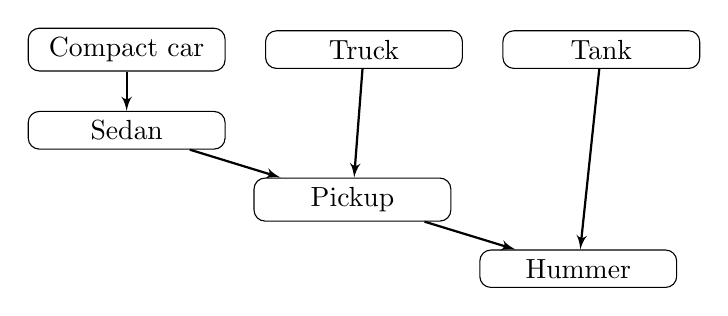
\begin{tikzpicture}
      [cars/.style={rectangle,draw=black,rounded corners,minimum width=2.5cm,node distance=0.5cm}]
      % place nodes
      \node[cars] (compact) {Compact car};
      \node[cars] (sedan) [below=of compact] {Sedan};
      \node[cars] (truck) [right=of compact] {Truck};
      \node[cars] (pickup) [below right= of sedan] {Pickup};
      \node[cars] (tank) [right=of truck] {Tank};
      \node[cars] (hummer) [below right= of pickup] {Hummer};
      % add edges
      \draw [-latex',thick] (compact) -- (sedan);
      \draw [-latex',thick] (sedan) -- (pickup);
      \draw [-latex',thick] (truck) -- (pickup);
      \draw [-latex',thick] (tank) -- (hummer);
      \draw [-latex',thick] (pickup) -- (hummer);
    \end{tikzpicture}
    \label{fig:car-hierarchy}
  }
  \hspace*{0.5cm}
  \subfloat[]{
    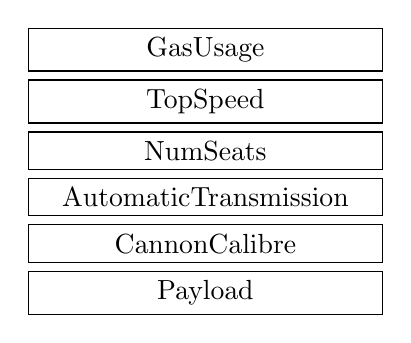
\begin{tikzpicture}
      [propertyBox/.style={rectangle,draw=black,minimum width=4.5cm,node distance=0.1cm}]
      \node[propertyBox] (gasUsage) {GasUsage};
      \node[propertyBox] (speed) [below=of gasUsage] {TopSpeed};
      \node[propertyBox] (seats) [below=of speed] {NumSeats};
      \node[propertyBox] (automatic) [below=of seats] {AutomaticTransmission};
      \node[propertyBox] (calibre) [below=of automatic] {CannonCalibre};
      \node[propertyBox] (payload) [below=of calibre] {Payload};
    \end{tikzpicture}
    \label{fig:car-propertynames}
  }
  \caption{\textbf{(a)}~A possible property inheritance graph for
    various kinds of cars.  The lower nodes inherit from higher ones;
    Inherited properties from nodes on the right take precedence over the
    properties defined on the left. \textbf{(b)}~Property names
    which make sense for at least one of the car types of (a).}
\end{figure}

Using the \Dumux property system, this inheritance hierarchy is
defined by:
\begin{lstlisting}[name=propsyscars,style=DumuxCode]
#include <dumux/common/propertysystem.hh>
#include <iostream>

namespace Dumux {
namespace Properties {
NEW_TYPE_TAG(CompactCar);
NEW_TYPE_TAG(Truck);
NEW_TYPE_TAG(Tank);
NEW_TYPE_TAG(Sedan, INHERITS_FROM(CompactCar));
NEW_TYPE_TAG(Pickup, INHERITS_FROM(Sedan, Truck));
NEW_TYPE_TAG(HummerH1, INHERITS_FROM(Pickup, Tank));
\end{lstlisting}

Figure \ref{fig:car-propertynames} lists a few property names which
make sense for at least one of the nodes of Figure
\ref{fig:car-hierarchy}. These property names can be declared as
follows:
\begin{lstlisting}[name=propsyscars,style=DumuxCode]
NEW_PROP_TAG(TopSpeed); // [km/h]
NEW_PROP_TAG(NumSeats); // []
NEW_PROP_TAG(CanonCaliber); // [mm]
NEW_PROP_TAG(GasUsage); // [l/100km]
NEW_PROP_TAG(AutomaticTransmission); // true/false
NEW_PROP_TAG(Payload); // [t]
\end{lstlisting}

\noindent
So far, the inheritance hierarchy and the property names are completely
separate. What is missing is setting some values for the property
names on specific nodes of the inheritance hierarchy. Let us assume
the following:
\begin{itemize}
\item For a compact car, the top speed is the gas usage in $\unitfrac{l}{100km}$
  times $30$, the number of seats is $5$ and the gas usage is
  $\unitfrac[4]{l}{100km}$.
\item A truck is by law limited to $\unitfrac[100]{km}{h}$ top speed, the number
  of seats is $2$, it uses $\unitfrac[18]{l}{100km}$ and has a cargo payload of
  $\unit[35]{t}$.
\item A tank exhibits a top speed of $\unitfrac[60]{km}{h}$, uses $\unitfrac[65]{l}{100km}$
  and features a $\unit[120]{mm}$ diameter canon
\item A sedan has a gas usage of $\unitfrac[7]{l}{100km}$, as well as an automatic
  transmission, in every other aspect it is like a compact car.
\item A pick-up truck has a top speed of $\unitfrac[120]{km}{h}$ and a payload of
  $\unit[5]{t}$. In every other aspect it is like a sedan or a truck but if in
  doubt, it is more like a truck.
\item The Hummer-H1 SUV exhibits the same top speed as a pick-up
  truck.  In all other aspects it is similar to a pickup and a tank,
  but, if in doubt, more like a tank.
\end{itemize}

\noindent
Using the \Dumux property system, these assumptions are formulated
using
\begin{lstlisting}[name=propsyscars,style=DumuxCode]
SET_INT_PROP(CompactCar, TopSpeed, GET_PROP_VALUE(TypeTag, GasUsage) * 30);
SET_INT_PROP(CompactCar, NumSeats, 5);
SET_INT_PROP(CompactCar, GasUsage, 4);

SET_INT_PROP(Truck, TopSpeed, 100);
SET_INT_PROP(Truck, NumSeats, 2);
SET_INT_PROP(Truck, GasUsage, 18);
SET_INT_PROP(Truck, Payload, 35);

SET_INT_PROP(Tank, TopSpeed, 60);
SET_INT_PROP(Tank, GasUsage, 65);
SET_INT_PROP(Tank, CanonCaliber, 120);

SET_INT_PROP(Sedan, GasUsage, 7);
SET_BOOL_PROP(Sedan, AutomaticTransmission, true);

SET_INT_PROP(Pickup, TopSpeed, 120);
SET_INT_PROP(Pickup, Payload, 5);

SET_INT_PROP(HummerH1, TopSpeed, GET_PROP_VALUE(TTAG(Pickup), TopSpeed));
\end{lstlisting}

\noindent
At this point, the Hummer-H1 has a $\unit[120]{mm}$ canon which it inherited
from its military ancestor. It can be removed by
\begin{lstlisting}[name=propsyscars,style=DumuxCode]
UNSET_PROP(HummerH1, CanonCaliber);

}} // close namespaces
\end{lstlisting}

\noindent
Now property values can be retrieved and some diagnostic messages can
be generated. For example
\begin{lstlisting}[name=propsyscars,style=DumuxCode]
int main()
{
    std::cout << "top speed of sedan: " << GET_PROP_VALUE(TTAG(Sedan), TopSpeed) << "\n";
    std::cout << "top speed of truck: " << GET_PROP_VALUE(TTAG(Truck), TopSpeed) << "\n";

    std::cout << PROP_DIAGNOSTIC(TTAG(Sedan), TopSpeed);
    std::cout << PROP_DIAGNOSTIC(TTAG(HummerH1), CanonCaliber);

    Dumux::Properties::print<TTAG(Sedan)>();
}
\end{lstlisting}
will yield the following output:
\begin{lstlisting}[style=Bash, basicstyle=\ttfamily\scriptsize\let\textcolor\textcolordummy]
$ top speed of sedan: 210
$ top speed of truck: 100
$ Properties for Sedan:
$   bool   AutomaticTransmission = 'true' defined at test_propertysystem.cc:68
$   int    GasUsage = '7' defined at test_propertysystem.cc:67
$   Inherited from CompactCar:
$     int    NumSeats = '5' defined at test_propertysystem.cc:55
$     int    TopSpeed = '::Dumux::Properties::GetProperty<TypeTag, ::Dumux::Properties::PTag::GasUsage>::p::value * 30' defined at test_propertysystem.cc:54
\end{lstlisting}

\subsection{Property and Parameter Values}
In \Dumux three different ways to obtain the value of a property are available:
\begin{description}
\item[\texttt{{\small GET\_PROP\_VALUE:}}]
Always returns the \emph{compile-time} specified value of the property. This is
needed for properties, which are not intended to be changed by parameter files.

\item[\texttt{{\small GET\_PARAM\_FROM\_GROUP:}}]
Returns the compile-time specified value, if this value is not be overwritten
by the parameter input file.

\item[\texttt{{\small GET\_RUNTIME\_PARAM\_FROM\_GROUP:}}]
Always returns a \emph{run-time} specified value. If the value is not specified
at run-time an error is thrown. This is needed for problem specific properties
or properties, which do not have a meaningful default value.
\end{description}

\section{Fluid Framework}
\label{sec:fluidframework}

\todo[inline]{Wie kann dieses Kapitel besser mit doxygen vereinbart werden? Evtl. durch generische
              Klassen in dumux, die dann automatische im doxygen auftauchen.}

This chapter discusses the \Dumux fluid framework. \Dumux users who
do not want to write new models and who do not need new fluid
configurations may skip this chapter.

In the chapter, a high level overview over the the principle concepts
is provided first, then some implementation details follow.

\subsection{Overview}

The \Dumux fluid framework currently features the following concepts
(listed roughly in their order of importance):

\begin{description}
\item[Fluid state:] Fluid states are responsible for representing the
  complete thermodynamic configuration of a system at a given spatial
  and temporal position. A fluid state always provides access methods
  to {\bf all} thermodynamic quantities, but the concept of a fluid state does not
  mandate what assumptions are made to store these thermodynamic
  quantities. What fluid states also do {\bf not} do is to make sure
  that the thermodynamic state which they represent is physically
  possible.
\item[Fluid system:] Fluid systems express the thermodynamic {\bf
    relations}\footnote{Strictly speaking, these relations are
    functions, mathematically.} between quantities. Since functions do
  not exhibit any internal state, fluid systems are stateless classes,
  i.e. all member functions are \texttt{static}. This is a conscious
  decision since the thermodynamic state of the system is expressed by
  a fluid state!
\item[Parameter cache:] Fluid systems sometimes require
  computationally expensive parameters for multiple relations. Such
  parameters can be cached using a so-called parameter
  cache. Parameter cache objects are specific for each fluid system
  but they must provide a common interface to update the internal
  parameters depending on the quantities which changed since the last
  update.
\item[Constraint solver:] Constraint solvers are auxiliary tools to
  make sure that a fluid state is consistent with some thermodynamic
  constraints. All constraint solvers specify a well defined set of
  input variables and make sure that the resulting fluid state is
  consistent with a given set of thermodynamic equations. See section
  \ref{sec:constraint_solvers} for a detailed description of the
  constraint solvers which are currently available in \Dumux.
\item[Equation of state:] Equations of state (EOS) are auxiliary
  classes which provide relations between a fluid phase's temperature,
  pressure, composition and density. Since these classes are only used
  internally in fluid systems, their programming interface is
  currently ad-hoc.
\item[Component:] Components are fluid systems which provide the
  thermodynamic relations for the liquid and gas phase of a single
  chemical species or a fixed mixture of species. Their main purpose
  is to provide a convenient way to access these quantities from
  full-fledged fluid systems. Components are not supposed to be used
  by models directly.
\item[Binary coefficient:] Binary coefficients describe the relations
  of a mixture of two components. Typical binary coefficients are
  \textsc{Henry} coefficients or binary molecular diffusion
  coefficients. So far, the programming interface for accessing binary
  coefficients has not been standardized in \Dumux.
\end{description}

\subsection{Fluid States}
Fluid state objects express the complete thermodynamic state of a
system at a given spatial and temporal position.

\subsubsection{Exported Constants}
All fluid states must export the following constants:
\begin{description}
\item[numPhases:] The number of fluid phases considered.
\item[numComponents:] The number of considered chemical species or pseudo-species.
\end{description}

\subsubsection{Accessible Thermodynamic Quantities}
Also, all fluid states must provide the following methods:
\begin{description}
\item[temperature():] The absolute temperature $T_\alpha$ of
  a fluid phase $\alpha$.
\item[pressure():] The absolute pressure $p_\alpha$ of a
  fluid phase $\alpha$.
\item[saturation():] The saturation $S_\alpha$ of a fluid phase
  $\alpha$. The saturation is defined as the pore space occupied by
  the fluid divided by the total pore space:
  \[
  \saturation_\alpha := \frac{\porosity \mathcal{V}_\alpha}{\porosity \mathcal{V}}
  \]
\item[moleFraction():] Returns the molar fraction $x^\kappa_\alpha$ of
  the component $\kappa$ in fluid phase $\alpha$. The molar fraction
  $x^\kappa_\alpha$ is defined as the ratio of the number of molecules
  of component $\kappa$ and the total number of molecules of the phase
  $\alpha$.
\item[massFraction():] Returns the mass fraction $X^\kappa_\alpha$ of
  component $\kappa$ in fluid phase $\alpha$. The mass fraction
  $X^\kappa_\alpha$ is defined as the weight of all molecules of a
  component divided by the total mass of the fluid phase. It is
  related with the component's mole fraction by means of the relation
  \[
  X^\kappa_\alpha = x^\kappa_\alpha \frac{M^\kappa}{\overline M_\alpha}\;,
  \]
  where $M^\kappa$ is the molar mass of component $\kappa$ and
  $\overline M_\alpha$ is the mean molar mass of a molecule of phase
  $\alpha$.
\item[averageMolarMass():] Returns $\overline M_\alpha$, the mean
  molar mass of a molecule of phase $\alpha$. For a mixture of $N > 0$
  components, $\overline M_\alpha$ is defined as
  \[
  \overline M_\alpha = \sum_{\kappa=1}^{N} x^\kappa_\alpha M^\kappa
  \]
\item[density():] Returns the density $\rho_\alpha$ of the fluid phase
  $\alpha$.
\item[molarDensity():] Returns the molar density $\rho_{mol,\alpha}$
  of a fluid phase $\alpha$. The molar density is defined by the mass
  density $\rho_\alpha$ and the mean molar mass $\overline M_\alpha$:
  \[
  \rho_{mol,\alpha} = \frac{\rho_\alpha}{\overline M_\alpha} \;.
  \]
\item[molarVolume():] Returns the molar volume $v_{mol,\alpha}$ of a
  fluid phase $\alpha$. This quantity is the inverse of the molar
  density.
\item[molarity():] Returns the molar concentration $c^\kappa_\alpha$
  of component $\kappa$ in fluid phase $\alpha$.
\item[fugacity():] Returns the fugacity $f^\kappa_\alpha$ of component
  $\kappa$ in fluid phase $\alpha$. The fugacity is defined as
  \[
  f_\alpha^\kappa := \Phi^\kappa_\alpha x^\kappa_\alpha p_\alpha \;,
  \]
  where $\Phi^\kappa_\alpha$ is the {\em fugacity
    coefficient}~\cite{reid1987}.  The physical meaning of fugacity
  becomes clear from the equation
  \[
  f_\alpha^\kappa = p_\alpha \exp\left\{\frac{\zeta^\kappa_\alpha}{R T_\alpha} \right\} \;,
  \]
  where $\zeta^\kappa_\alpha$ represents the $\kappa$'s chemical
  potential in phase $\alpha$, $R$ stands for the ideal gas constant,
  and $T_\alpha$ for the absolute temperature of phase
  $\alpha$. Assuming thermal equilibrium, there is a one-to-one
  mapping between a component's chemical potential
  $\zeta^\kappa_\alpha$ and its fugacity $f^\kappa_\alpha$. In this
  case chemical equilibrium can thus be expressed by
  \[
  f^\kappa := f^\kappa_\alpha = f^\kappa_\beta\quad\forall \alpha, \beta
  \]
\item[fugacityCoefficient():] Returns the fugacity coefficient
  $\Phi^\kappa_\alpha$ of component $\kappa$ in fluid phase $\alpha$.
\item[enthalpy():] Returns specific enthalpy $h_\alpha$ of a fluid
  phase $\alpha$.
\item[internalEnergy():] Returns specific internal energy $u_\alpha$
  of a fluid phase $\alpha$. The specific internal energy is defined
  by the relation
  \[
  u_\alpha = h_\alpha - \frac{p_\alpha}{\rho_\alpha}
  \]
\item[viscosity():] Returns the dynamic viscosity
  $\mu_\alpha$ of fluid phase $\alpha$.
\end{description}

\subsubsection{Available Fluid States}
\todo{Diese Liste von verfügbaren \emph{FluidStates} sollte eigentlich so und 
      in gleicher Ausfgührlichkeit im doxygen möglich sein -$>$ deshalb raus.}
Currently, the following fluid states are provided by \Dumux:
\begin{description}
\item[NonEquilibriumFluidState:] This is the most general fluid state
  supplied. It does not assume thermodynamic equilibrium and thus
  stores all phase compositions (using mole fractions), fugacity
  coefficients, phase temperatures, phase pressures, saturations and
  specific enthalpies.
\item[CompositionalFluidState:] This fluid state is very similar to
  the \texttt{Non\-Equilibrium\-Fluid\-State} with the difference that
  the \texttt{Compositional\-Fluid\-State} assumes thermodynamic
  equilibrium. In the context of multi-phase flow in porous media,
  this means that only a single temperature needs to be stored.
\item[ImmisicibleFluidState:] This fluid state assumes that the fluid
  phases are immiscible, which implies that the phase compositions and
  the fugacity coefficients do not need to be stored explicitly.
\item[PressureOverlayFluidState:] This is a so-called {\em overlay}
  fluid state. It allows to set the pressure of all fluid phases but
  forwards everything else to another fluid state.
\item[SaturationOverlayFluidState:] This fluid state is like the
  \texttt{PressureOverlayFluidState}, except that the phase
  saturations are settable instead of the phase pressures.
\item[TempeatureOverlayFluidState:] This fluid state is like the
  \texttt{PressureOverlayFluidState}, except that the temperature is
  settable instead of the phase pressures. Note that this overlay
  state assumes thermal equilibrium regardless of underlying fluid
  state.
\item[CompositionOverlayFluidState:] This fluid state is like the
  \texttt{PressureOverlayFluidState}, except that the phase
  composition is settable (in terms of mole fractions) instead of the
  phase pressures.
\end{description}

\subsection{Fluid Systems}

Fluid systems express the thermodynamic relations between the
quantities of a fluid state.

\subsubsection{Parameter Caches}

All fluid systems must export a type for their \texttt{ParameterCache}
objects. Parameter caches can be used to cache parameter that are
expensive to compute and are required in multiple thermodynamic
relations. For fluid systems which do need to cache parameters,
\Dumux provides a \texttt{NullParameterCache} class.

The actual quantities stored by parameter cache objects are specific
to the fluid system and no assumptions on what they provide should be
made outside of their fluid system. Parameter cache objects provide a
well-defined set of methods to make them coherent with a given fluid
state, though. These update are:
\begin{description}
\item[updateAll(fluidState, except):] Update all cached quantities for
  all phases. The \texttt{except} argument contains a bit field of the
  quantities which have not been modified since the last call to a
  \texttt{update()} method.
\item[updateAllPresures(fluidState):] Update all cached quantities
  which depend on the pressure of any fluid phase.
\item[updateAllTemperatures(fluidState):] Update all cached quantities
  which depend on temperature of any fluid phase.
\item[updatePhase(fluidState, phaseIdx, except):] Update all cached
  quantities for a given phase. The quantities specified by the
  \texttt{except} bit field have not been modified since the last call
  to an \texttt{update()} method.
\item[updateTemperature(fluidState, phaseIdx):] Update all cached
  quantities which depend on the temperature of a given phase.
\item[updatePressure(fluidState, phaseIdx):] Update all cached
  quantities which depend on the pressure of a given phase.
\item[updateComposition(fluidState, phaseIdx):] Update all cached
  quantities which depend on the composition of a given phase.
\item[updateSingleMoleFraction(fluidState, phaseIdx, compIdx):] Update
  all cached quantities which depend on the value of the mole fraction
  of a component in a phase.
\end{description}
Note, that the parameter cache interface only guarantees that if a
more specialized \texttt{update()} method is called, it is not slower
than the next more-general method (e.g. calling
\texttt{updateSingleMoleFraction()} may be as expensive as
\texttt{updateAll()}). It is thus advisable to rather use a more
general \texttt{update()} method once than multiple calls to
specialized \texttt{update()} methods.

To make usage of parameter caches easier for the case where all cached
quantities ought to be re-calculated if a quantity of a phase was
changed, it is possible to only define the \texttt{updatePhase()}
method and derive the parameter cache from
\texttt{Dumux::ParameterCacheBase}.

\subsubsection{Exported Constants and Capabilities}

Besides providing the type of their \texttt{ParameterCache} objects,
fluid systems need to export the following constants and auxiliary
methods:
\begin{description}
\item[numPhases:] The number of considered fluid phases.
\item[numComponents:] The number of considered chemical (pseudo-)
  species.
\item[init():] Initialize the fluid system. This is usually used to
  tabulate some quantities
\item[phaseName():] Given the index of a fluid phase, return its name
  as human-readable string.
\item[componentName():] Given the index of a component, return its
  name as human-readable string.
\item[isLiquid():] Return whether the phase is a liquid, given the
  index of a phase.
\item[isIdealMixture():] Return whether the phase is an ideal mixture,
  given the phase index. In the context of the \Dumux fluid
  framework a phase $\alpha$ is an ideal mixture if, and only if, all
  its fugacity coefficients $\Phi^\kappa_\alpha$ do not depend on the
  phase composition. (Although they might very well depend on
  temperature and pressure.)
\item[isIdealGas():] Return whether a phase $\alpha$ is an ideal gas,
  i.e. it adheres to the relation
  \[
  p_\alpha v_{mol,\alpha} = R T_\alpha \;,
  \]
  with $R$ being the ideal gas constant.
\item[isCompressible():] Return whether a phase $\alpha$ is
  compressible, i.e. its density depends on pressure $p_\alpha$.
\item[molarMass():] Given a component index, return the molar mass of
  the corresponding component.
\end{description}

\subsubsection{Thermodynamic Relations}

Fluid systems have been explicitly designed to provide as few
thermodynamic relations as possible. A full-fledged fluid system thus
only needs to provide the following thermodynamic relations:
\begin{description}
\item[density():] Given a fluid state, an up-to-date parameter cache
  and a phase index, return the mass density $\rho_\alpha$ of the
  phase.
\item[fugacityCoefficient():] Given a fluid state, an up-to-date
  parameter cache as well as a phase and a component index, return the
  fugacity coefficient $\Phi^\kappa_\alpha$ of a the component for the
  phase.
\item[viscosity():] Given a fluid state, an up-to-date parameter cache
  and a phase index, return the dynamic viscosity $\mu_\alpha$ of the
  phase.
\item[diffusionCoefficient():] Given a fluid state, an up-to-date
  parameter cache, a phase and a component index, return the calculate
  the molecular diffusion coefficient for the component in the fluid
  phase.

  Molecular diffusion of a component $\kappa$ in phase $\alpha$ is
  caused by a gradient of the chemical potential and follows the law
  \[
  J^\kappa_\alpha = - D^\kappa_\alpha\ \mathbf{grad} \zeta^\kappa_\alpha\;,
  \]
  where $\zeta^\kappa_\alpha$ is the component's chemical potential,
  $D^\kappa_\alpha$ is the diffusion coefficient and $J^\kappa_\alpha$
  is the diffusive flux. $\zeta^\kappa_\alpha$ is connected to the
  component's fugacity $f^\kappa_\alpha$ by the relation
  \[
  \zeta^\kappa_\alpha =
  R T_\alpha \mathrm{ln} \frac{f^\kappa_\alpha}{p_\alpha} \;.
  \]
\item[binaryDiffusionCoefficient():] Given a fluid state, an
  up-to-date parameter cache, a phase index and two component indices,
  return the binary diffusion coefficient for the binary mixture. This
  method is less general than \texttt{diffusionCoefficient} method,
  but relations can only be found for binary diffusion coefficients in
  the literature.
\item[enthalpy():] Given a fluid state, an up-to-date parameter cache
  and a phase index, this method calulates the specific enthalpy
  $h_\alpha$ of the phase.
\item[thermalConductivity:] Given a fluid state, an up-to-date
  parameter cache and a phase index, this method returns the thermal
  conductivity $\lambda_\alpha$ of the fluid phase. The thermal
  conductivity is defined by means of the relation
  \[
  \dot Q = \lambda_\alpha \mathbf{grad}\;T_\alpha \;,
  \]
  where $\dot Q$ is the heat flux caused by the temperature gradient
  $\mathbf{grad}\;T_\alpha$.
\item[heatCapacity():] Given a fluid state, an up-to-date parameter
  cache and a phase index, this method computes the isobaric heat
  capacity $c_{p,\alpha}$ of the fluid phase. The isobaric heat
  capacity is defined as the partial derivative of the specific
  enthalpy $h_\alpha$ to the fluid pressure:
  \[
  c_{p,\alpha} = \frac{\partial h_\alpha}{\partial p_\alpha}
  \]
  % TODO: remove the heatCapacity() method??
\end{description}

Fluid systems may chose not to implement some of these methods and
throw an exception of type \lstinline{Dune::NotImplemented} instead. Obviously,
such fluid systems cannot be used for models that depend on those
methods.

\subsubsection{Available Fluid Systems}
\todo{Diese Liste von verfügbaren \emph{FluidSystems} sollte eigentlich so und 
      in gleicher Ausfgührlichkeit im doxygen möglich sein -$>$ deshalb raus.}

Currently, the following fluid systems are available in \Dumux:
\begin{description}
\item[Dumux::FluidSystems::TwoPImmiscible:] A two-phase fluid system
  which assumes immiscibility of the fluid phases. The fluid phases
  are thus completely specified by means of their constituting
  components. This fluid system is intended to be used with models
  that assume immiscibility.
\item[Dumux::FluidSystems::H2ON2:] A two-phase fluid system featuring
  gas and liquid phases and distilled water ($H_2O$) and pure
  molecular Nitrogen ($N_2$) as components.
\item[Dumux::FluidSystems::H2OAir:] A two-phase fluid system
  featuring gas and liquid phases and distilled water ($H_2O$) and
  air (Pseudo component composed of $79\%\;N_2$, $20\%\;O_2$ and
  $1\%\;Ar$) as components.
\item[Dumux::FluidSystems::H2OAirMesitylene:] A three-phase fluid
  system featuring gas, NAPL and water phases and distilled water, air
  and Mesitylene ($C_6H_3(CH_3)_3$) as components. This fluid system
  assumes all phases to be ideal mixtures.
\item[Dumux::FluidSystems::H2OAirXylene:] A three-phase fluid system
  featuring gas, NAPL and water as phases and distilled water, air and
  Xylene ($C_8H_{10}$) as components. This fluid system assumes all
  phases to be ideal mixtures.
\item[Dumux::FluidSystems::Spe5:] A three-phase fluid system featuring
  gas, oil and water as phases and the seven components distilled
  water, Methane ($C_1$), Propane ($C_3$), Pentane ($C_5$), Heptane
  ($C_7$), Decane ($C_{10}$), Pentadecane ($C_{15}$) and Icosane
  ($C_{20}$). For the water phase the IAPWS-97 formulation is used as
  equation of state, while for the gas and oil phases a
  \textsc{Peng}-\textsc{Robinson} equation of state with slightly
  modified parameters is used. This fluid system is highly non-linear,
  and the gas and oil phases also cannot be considered ideal
  mixtures\cite{SPE5}.
\end{description}

\subsection{Constraint Solvers}
\label{sec:constraint_solvers}

Constraint solvers connect the thermodynamic relations expressed by
fluid systems with the thermodynamic quantities stored by fluid
states. Using them is not mandatory for models, but given the fact
that some thermodynamic constraints can be quite complex to solve,
sharing this code between models makes sense. Currently, \Dumux
provides the following constraint solvers:
\begin{description}
\item[CompositionFromFugacities:] This constraint solver takes all
  component fugacities, the temperature and pressure of a phase as
  input and calculates the composition of the fluid phase. This means
  that the thermodynamic constraints used by this solver are
  \[
  f^\kappa = \Phi^\kappa_\alpha(\{x^\beta_\alpha \}, T_\alpha, p_\alpha)  p_\alpha x^\kappa_\alpha\;,
  \]
  where ${f^\kappa}$, $T_\alpha$ and $p_\alpha$ are fixed values.
\item[ComputeFromReferencePhase:] This solver brings all
  fluid phases into thermodynamic equilibrium with a reference phase
  $\beta$, assuming that all phase temperatures and saturations have
  already been set. The constraints used by this solver are thus
  \begin{eqnarray*}
  f^\kappa_\beta = f^\kappa_\alpha = \Phi^\kappa_\alpha(\{x^\beta_\alpha \}, T_\alpha, p_\alpha)  p_\alpha x^\kappa_\alpha\;, \\
  p_\alpha = p_\beta + p_{c\beta\alpha} \;,
  \end{eqnarray*}
  where $p_{c\beta\alpha}$ is the capillary pressure between the
  fluid phases $\beta$ and $\alpha$.
\item[CompositionalFlash:] A compositional 2p2c flash solver for the
sequential models in \Dumux. Input is temperature, phase pressures
and feed mass fraction, the solver computes the compositional variables and
saturations.
\item[NcpFlash:] This is a so-called flash solver. A flash solver
  takes the total mass of all components per volume unit and the phase
  temperatures as input and calculates all phase pressures,
  saturations and compositions. This flash solver works for an
  arbitrary number of phases $M > 0$ and components $N \geq M - 1$. In
  this case, the unknown quantities are the following:
  \begin{itemize}
  \item $M$ pressures $p_\alpha$
  \item $M$ saturations $\saturation_\alpha$
  \item $M\cdot N$ mole fractions $x^\kappa_\alpha$
  \end{itemize}
  This sums up to $M\cdot(N + 2)$. The equations side of things
  provides:
  \begin{itemize}
  \item $(M - 1)\cdot N$ equations stemming from the fact that the
    fugacity of any component is the same in all phases, i.e.
    \[
    f^\kappa_\alpha = f^\kappa_\beta
    \]
    holds for all phases $\alpha, \beta$ and all components $\kappa$.
  \item $1$ equation comes from the fact that the whole pore space is
    filled by some fluid, i.e.
    \[
    \sum_{\alpha=1}^M \saturation_\alpha = 1
    \]
  \item $M - 1$ constraints are given by the capillary pressures:
    \[
    p_\beta = p_\alpha + p_{c\beta\alpha} \;,
    \]
    for all phases $\alpha$, $\beta$
  \item $N$ constraints come the fact that the total mass of each
    component is given:
    \[
    c^\kappa_{tot} = \sum_{\alpha=1}^M x_\alpha^\kappa\;\rho_{mol,\alpha} = const
    \]
  \item And finally $M$ model assumptions are used. This solver uses
    the NCP constraints proposed in~\cite{LHHW2011}:
    \[
     0 = \mathrm{min}\{\saturation_\alpha, 1 - \sum_{\kappa=1}^N x_\alpha^\kappa\}
   \]
\end{itemize}
The number of equations also sums up to $M\cdot(N + 2)$. Thus, the
system of equations is closed.
\item[ImmiscibleFlash:] This is a flash solver assuming immiscibility
  of the phases. It is similar to the \texttt{NcpFlash} solver but a
  lot simpler.
\item[MiscibleMultiphaseComposition:] This solver calculates the
  composition of all phases provided that each of the phases is
  potentially present. Currently, this solver does not support
  non-ideal mixtures.
\end{description}

\section{Grid Handling}
\label{sec:gridhandling}

This section summarizes some ideas about grid generation and grid formats that can be used by \Dumux. In general,
\Dumux can read grids from file, or, construct grids inside the code. All grids are constructed inside a so called \texttt{GridCreator} which is a \Dumux property.
Note that some \texttt{GridCreator}s are already available in \Dumux, so e.g.
construction of a structured grid is fairly easy. We will subsequently introduce the supported file formats, the standard grid creator and its capabilities,
and briefly mention how to customize and deal with common other grid formats.

\subsection{Supported file formats}
\Dumux can read grids from file using the Dune Grid Format (DGF) or the Gmsh mesh format.

\subsubsection{Dune Grid Format}
Most of our \Dumux tests and tutorials use the Dune Grid Format (DGF) to read in grids. A detailed description
of the DGF format and some examples can be found in the \Dune doxygen documentation
\textbf{(Modules $\rightarrow$ I/O $\rightarrow$ Dune Grid Format (DGF)}). To generate larger or more
complex DGF files, we recommend to write your own scripts, e.g in \Cplusplus, Matlab or Python.

The DGF format can also used to read in spatial parameters defined on the grid. These parameters can
be defined on nodes as well as on the elements. An example for predefined parameters on a grid is
the \texttt{test\_boxco2} or \texttt{test\_cco2} in the  \texttt{dumux/test/porousmediumflow/co2/implicit/} folder.

\subsubsection{Gmsh Mesh Format}
Gmsh is an open-source flexible grid generator for unstructured finite-element meshes (\cite{GEUZAINE2009}, \url{http://geuz.org/gmsh/}).
\Dumux supports the default Gmsh mesh format (MSH). For the format specifics and how to create grids with Gmsh, e.g. using
the provided GUI, we refer to the Gmsh documentation (\url{http://geuz.org/gmsh/doc/texinfo/gmsh.html}).

The MSH format can contain element and boundary markers defined in the grid. Thus, boundaries can be easily marked as e.g. inflow boundaries
using Gmsh. Further, the format supports higher order elements. They can be used to create boundary parameterization supported by e.g. the grid
manager \texttt{UGGrid}.
An example can be found in \texttt{dumux/test\allowbreak/io/gridcreator}.



\subsection{The default \texttt{GridCreator}}
The default \texttt{GridCreator} is called \texttt{GridCreator} and is automatically avaible in all problems.
It can construct grids from a DGF file (*.dgf) by simply providing the filename to the grid in the \texttt{Grid} group~\footnote{Note
that group name \texttt{Grid} is the default group name and can be customized in your problem changing the string property \texttt{GridParameterGroup}.
This way it is possible, e.g. for problems with more than one grid, to set different group names for each grid, thus configuring them separately.}
of the input file:
\begin{lstlisting}[style=DumuxParameterFile]
[Grid]
File = mydgfgrid.dgf
\end{lstlisting}
If you are using an unstructured grid manager like \texttt{UGGrid} or \texttt{ALUGrid}, constructing a grid from a Gmsh mesh file (*.msh) is just changing a line:
\begin{lstlisting}[style=DumuxParameterFile]
[Grid]
File = mygmshgrid.msh
\end{lstlisting}
\Dumux will tell you in case your selected grid manager does not support reading Gmsh files. You want to intially refine your grid? It's just adding a line:
\begin{lstlisting}[style=DumuxParameterFile]
[Grid]
File = mydgfgrid.dgf
Refinement = 4
\end{lstlisting}
When reading a Gmsh file, further parameters are recognized. \texttt{Verbose} enables verbose output on grid construction when set to $1$.
\texttt{BoundarySegments} enables reading parametrized boundaries. \texttt{PhysicalEntities} enables reading boundary and element flags.

\subsubsection{Grid manager specific parameters}
The default \texttt{GridCreator} supports also a selection of grid specific parameters.
To give an example we look at the commonly used unstructured grid manager \texttt{UGGrid}.
\texttt{UGGrid}s support red-green refinement per default. One can turn off the green closure by setting the grid's closure type
\begin{lstlisting}[style=DumuxParameterFile]
[Grid]
File = mydgfgrid.dgf
ClosureType = None # or Green
\end{lstlisting}
For all available parameters see the Doxygen documentation.

\subsubsection{Structured grids}
If you want to construct a structured grid with the default grid creator instead of the \texttt{File} key supply
\begin{lstlisting}[style=DumuxParameterFile]
[Grid]
LowerLeft = 0 0 0
UpperRight = 1 1 1
Cells = 10 10 20
\end{lstlisting}
where \texttt{LowerLeft} is a vector to the lower left corner of the grid and \texttt{UpperRight} a vector to the upper right corner.
\texttt{Cells} is a vector with the number of cells in each coordinate direction. Note that for a grid in a two-dimensional world, the
vectors only have two entries.

Depending on the grid manager further parameters are recognized.
\texttt{UGGrid}s, for example, supports simplex elements as well as hexahedral elements
(called simplified ``cube'' in \Dune). When creating a structured grid, we can select the cell type as follows
\begin{lstlisting}[style=DumuxParameterFile]
[Grid]
LowerLeft = 0 0 0
UpperRight = 1 1 1
Cells = 10 10 20
CellType = Cube # or Simplex
\end{lstlisting}
For all available parameters see the Doxygen documentation.

\subsection{Other grid formats and customized grid creators}
Other grid formats than DGF and MSH have to be converted to DGF or MSH to be read into \Dumux. A second possiblity (advanced \Cplusplus) is to write your own
\texttt{GridCreator}. For examples have a look at the \texttt{CubeGridCreator} for a simple and the \texttt{ArtGridCreator} for a more complex example.
It follows a (non-comprehensive) list of hints for some other common grid formats.

\subsubsection{Petrel}
Grids from Petrel (in ASCII format with the extension *.GRDECL) can be imported into \Dumux in two ways:
  \begin{enumerate}
  \item Using the GRDECL format directly with the help of the grid-manager \texttt{dune-cornerpoint}.
  \item Converting the GRDECL file into the DGF format.
  \end{enumerate}
The fist options requires the installation of \texttt{dune-cornerpoint} along with its dependencies. Set the property \texttt{Grid} to \texttt{Dune::CpGrid} in your problem file.

The second option has the advantage that you end up with a DGF which can then be used with any grid-manager (\texttt{dune-alugrid}, \texttt{UG} etc.) You also have to install \texttt{dune-cornerpoint}. Additionally you have to modify the converter \texttt{grdecl2vtu} found in \texttt{dune-cornerpoint/examples} to also write a DGF. To do so you have to:
\begin{itemize}
 \item Include the \texttt{dgfwriter.hh} found in \texttt{dune-grid/dune/grid/io/file/dgfparser}
 \item Create an object of the \texttt{Dune::DGFWriter} and call the its function \texttt{write()} within the \texttt{main} function for example after the \texttt{vtkwriter()} is called:
\begin{lstlisting}[style=DumuxCode]
Dune::DGFWriterParam<CpGrid::LeafGridView> dgfWriter(grid.leafView()))
dgfWriter.write(fnamebase + ".dgf")
\end{lstlisting}
\end{itemize}
Material parameters for elements with Petrel specific keywords like \texttt{PORO} are parsed by the converter \texttt{grdecl2vtu} (see the \texttt{main} function). They are available as vectors within the \texttt{main} function. The main GRDECL file with the coordinates must include the GRDECL files of the parameters, if for example the parameters are not already included, include the file bearing your parameter in your main GRDECL file:
\begin{lstlisting}
INCLUDE
'PARAMETER_X.GRDECL'
/
\end{lstlisting}
To add the parameters to your DGF you have to make changes to the header \texttt{dgfwriter.hh} such that they are passed as arguments of the \texttt{write()} function and written after each element (modify \texttt{writeElement()} and internal \texttt{write()} functions accordingly). Take caution that you stick to the correct DGF syntax (see \textbf{Modules $\rightarrow$ I/O $\rightarrow$ Dune Grid Format (DGF)} for reference).

\subsubsection{ArtMesh}
\href{http://www.topologica.org/toplog/wp/}{ArtMesh} is a 3D mesh generation software. It has its own mesh file format
which can be read by \Dumux via the \texttt{ArtGridCreator}. Traditionally it was used within \Dumux for fracture simulations with
the discrete fracture matrix model (\texttt{2pdfm}). A detailed description of the fracture network creation and gridding
can be found for example in \cite{Tatomir2012a}, pp. 68.

\subsubsection{ICEM}
For complex geometries a graphical tool to create grids might be appropriate. One possibility to mesh for example CAD
geometry data is the commercial software \href{http://www.ansys.com/Products/Other+Products/ANSYS+ICEM+CFD/}{ANSYS ICEM
CFD}. A very detailed, but outdated description can be found at the LH2 internal wiki. A more recent best practice guide is available
in dumux-devel at dumux-devel/util/gridconverters/Documentation\_ICEM\_CFD\_create\_mesh.odt. At LH2 exists a script which converts the ICEM mesh into the DGF.


\bibliographystyle{plain}
\bibliography{dumux-handbook}
\printindex
\end{document}
